\documentclass[10pt, a4paper]{article} % Standard academic font size and paper

% --- Page Margins & Padding ---
% Standard 1-inch (2.54cm) margins are typical for this kind of report.
\usepackage[top=2.5cm, bottom=2.5cm, left=2.5cm, right=2.5cm]{geometry}

% --- Line Spacing ---
\usepackage{setspace}
\setstretch{1.15} % Slight padding between lines for readability

% --- Headers and Footers ---
% The document features "HPC Project Report" and "Page X of Y"
\usepackage{fancyhdr}
\usepackage{lastpage}
\pagestyle{fancy}
\fancyhf{} % Clear default headers/footers
\fancyhead[L]{Matrix Multiplication Parallelization} % Top Left
\fancyhead[R]{HPC Project Report} % Top Right
\fancyfoot[C]{\thepage\ of \pageref{LastPage}} % Bottom Center (e.g., 2 of 38)
\renewcommand{\headrulewidth}{0.4pt} % Line under header
\renewcommand{\footrulewidth}{0pt}

% --- Fonts and Typography ---
\usepackage[utf8]{inputenc}
\usepackage[T1]{fontenc}
\usepackage{lmodern} % Standard Latin Modern font
\usepackage{microtype} % Improves text justification and kerning
\usepackage[title]{appendix}

% --- Math Settings ---
\usepackage{amsmath, amssymb, amsthm}

% --- Code Block Settings ---
% The document has C and CUDA code snippets. 
\usepackage{threeparttable}
\usepackage{listings}
\usepackage{booktabs}
\usepackage{xcolor}
\lstdefinestyle{CStyle}{
    language=C,
    basicstyle=\ttfamily\small,
    keywordstyle=\color{blue}\bfseries,
    commentstyle=\color{gray},
    stringstyle=\color{red},
    numbers=left,
    numberstyle=\tiny\color{gray},
    stepnumber=1,
    numbersep=8pt,
    backgroundcolor=\color{white},
    showspaces=false,
    showstringspaces=false,
    showtabs=false,
    frame=single,
    tabsize=4,
    captionpos=b,
    breaklines=true,
    breakatwhitespace=false,
    escapeinside={(*@}{@*)} % This defines the delimiters for LaTeX code
}

\usepackage[backend=biber, style=ieee]{biblatex}
\addbibresource{references.bib}

% --- Tables and Figures ---
\usepackage{graphicx}
\usepackage{float}
\usepackage{booktabs} % For professional-looking tables
\usepackage{caption}
\captionsetup{font=small, labelfont=bf} % e.g., "Table 1:" in bold


\title{\huge{\textbf{High Performance Computing} \\ 
    Matrix Multiplication Analysis \& Parallelization}}
\author{Luca Ninivaggi (S5312342) \\
    Flavio Barrara Stefani (S5175710) \\
    Isabella Tagliafico (S4644488)
    \date{}
    }

\begin{document}


\maketitle
\begin{abstract}
\noindent
The following report explores the entire analysis about the execution and optimization of matrix multiplication algorithms. Starting from a reference sequential implementation and moving across various compiling optimizations, we after mode over different parallel programming paradigms: shared-memory (OpenMP), GPU-accelerated (CUDA) and distributed-memory (MPI).
\end{abstract} 

\tableofcontents

\section{Introduction}

\subsection{Problem definition}

Matrix Multiplication (MM) is a fundamental high-performance computing (HPC) kernel, widely used to benchmark parallel architectures due to its high arithmetic intensity. For square matrices $A, B \in \mathbb{R}^{n \times n}$, the product $C \in \mathbb{R}^{n \times n}$ is defined as:
\begin{equation}
    C_{ij} = \sum_{k=1}^{n} A_{ik} B_{kj} \qquad \text{for} \quad 1 \le i, j \le n
\end{equation}

Computing a single element $C_{ij}$ requires a dot product between the $i$-th row of $A$ and the $j$-th column of $B$, involving exactly $n$ multiplications and $n-1$ additions. Therefore, calculating one element takes approximately $2n$ floating-point operations (FLOPs). 

Since the matrix $C$ contains $n^2$ elements, the total arithmetic cost is $n^2 \times 2n = 2n^3$ FLOPs, hence complexity of $\mathcal{O}(n^3)$. 

The objective of this project is to analyze and optimize MM performance through iterative parallelization\footnote{Different algorithms are used to implement the Matrix Multiplication; their in-depth description can be found in Appendix~\ref{app:algorithms}.}. 


\subsection{Roadmap}\label{subsec:iterative_improvements}

Starting from a sequential baseline for matrix multiplication, we progressively introduce hardware-aware optimizations using OpenMP, CUDA, and MPI. 
To approach peak theoretical performance, the execution is iteratively optimized by exploiting the hierarchy of parallelism in modern High-Performance Computing (HPC) systems:

\begin{itemize}
    \item \textbf{Instruction and Vector Level (SIMD):} The simultaneous execution of operations (e.g., FMA: $a + (b \times c)$) and the application of single instructions to multiple data points via registers. This is exploited at the core level through aggressive compiler optimizations and explicit AVX intrinsics in Section~\ref{sec:sequential}.
    
    \item \textbf{Hyperthreading and Core Level:} The utilization of multiple logical threads sharing execution resources, alongside independent physical processing units on a CPU. This is leveraged by using OpenMP (Section~\ref{sec:openmp}), to distribute the workload across available threads and cores.
    
    \item \textbf{Accelerator Level:} The offloading of heavily data-parallel tasks to specialized hybrid hardware. This is addressed by executing the matrix blocks on the GPU utilizing CUDA (Section~\ref{sec:CUDA}).
    
    \item \textbf{Node Level:} The utilization of individual computers connected via high-speed interconnects within a cluster. This is managed using MPI (Section~\ref{sec:mpi}) to partition and distribute the overall computation across multiple discrete nodes\footnote{While the proposed implementation could actually run a distributed framework, due to hardware limitation all the tests were made on a single machine.}.
\end{itemize}



In theory, this parallelization strategy could be further extended to exploit multi-socket architectures (multiple physical CPUs on a single node) and Grid/Cloud distributions (multiple systems linked over a network for massive workloads). However, these specific levels are omitted due to the lack of hardware capabilities.

\section{Experimental Setup}

This section describes the experimental framework adopted, providing a detailed overview of the hardware configuration, software stack, and experimental procedures used in this study.



% =========================================================
% ===================== HARDWARE ==========================
% =========================================================

\subsection{Hardware Platform}

\subsubsection{CPU Hardware Specifications (University Lab)}
All CPU-based experiments (sequential, OpenMP and MPI implementations) were conducted on the laboratory workstations of the University of Genoa. 
The main architectural characteristics of the processors are reported in Table~\ref{tab:cpu_specs}.


\paragraph{CPU topology (hwloc).}
In addition to \texttt{lscpu}, we used \texttt{lstopo} (hwloc) to inspect the CPU topology, including the mapping between physical cores, hardware threads (PUs), and cache hierarchy.
The results of the analysis of this topology are integrated with those reported in Table~\ref{tab:cpu_specs}.

\begin{table}[H]
\centering
\caption{CPU hardware specifications of the laboratory workstation.}
\label{tab:cpu_specs}
\begin{tabular}{ll}
\toprule
\textbf{Component} & \textbf{Specification} \\
\midrule
Processor Model & Intel Core i9-12900K (12th Gen, Alder Lake) \\
Microarchitecture & Hybrid (8 Performance cores + 8 Efficient cores) \\
Instruction Set Architecture & x86\_64 \\
Sockets & 1 \\
Physical Cores & 16 \\
Logical Threads & 24 \\
Threads per Core & 2 (P-cores), 1 (E-cores) \\
Base/Max Frequency & 0.8 GHz -- 4.02 GHz \\
L1 Data Cache & 640 KiB Total (16 instances, 12-way associative, 64 B line size) \\
L1 Instruction Cache & 768 KiB Total (16 instances, 8-way associative, 64 B line size) \\
L2 Cache & 14 MiB Total (10 instances, 10-way associative, 64 B line size) \\
Shared L3 Cache & 30 MiB (12-way associative, 64 B line size) \\
SIMD Extensions & SSE, SSE2, SSE4.1/4.2, AVX, AVX2, FMA \\
NUMA Nodes & 1 \\
\bottomrule
\end{tabular}
\end{table}

The platform features an asymmetric hybrid core design combining 8 \emph{Performance cores} (P-cores, supporting 2-way simultaneous multithreading) and 8 \emph{Efficient cores} (E-cores, single-threaded), yielding a total of 24 logical CPUs\footnote{In Intel's hybrid architecture Performance cores are optimized for single-threaded execution speed and low latency, whereas Efficient cores are designed to maximize multi-threaded throughput and power efficiency per watt.}. 

Furthermore, the cache hierarchy is heterogeneous: P-cores possess private L2 caches, whereas E-cores are grouped into clusters that share a common L2 cache.


\subsubsection{GPU Hardware Specifications (Google Colab)}\label{sec:GPU spec}
CUDA experiments were conducted using Google Colab. 


The specifications of the device used for the experiments are reported in Table~\ref{tab:gpu_specs_colab}. The NVIDIA Tesla T4 is based on the Turing architecture (compute capability 7.5) and features 40 Streaming Multiprocessors (SMs), for a total of 2560 CUDA cores and 320 Tensor cores. 

The device provides approximately 8.1 TFLOP/s of theoretical single-precision (FP32) performance and a peak memory bandwidth of about 320 GB/s using GDDR6 memory.

While the T4 is capable of approximately 8.1 TFLOP/s in single-precision (FP32), in our study we explicitly focus on double-precision (FP64) implementations.  
It is also important to acknowledge that the onboard \emph{Tensor Cores} allow for heavily optimized matrix multiplications when utilizing libraries (such as \texttt{cuBLAS})\footnote{Tensor Cores are specialized execution units designed to compute dense matrix-multiply-and-accumulate (MMA) operations at the hardware level in a single clock cycle. In this study we did not use them since they do not support the FP64 precision.}.


\paragraph{Hardware Profiling}
It should be noted that some architectural parameters, including the number of Streaming Multiprocessors, CUDA cores, tensor cores, peak FP32 throughput, and theoretical memory bandwidth, are not directly obtainable via \texttt{nvidia-smi}. 
These values were derived from the official NVIDIA Tesla T4 technical documentation and datasheet.

Since Google Colab dynamically assigns GPU resources, the reported specifications correspond to the device allocated during the experimental session and may vary across different sessions.

\begin{table}[H]
\centering
\caption{GPU hardware specifications of the Google Colab environment.}
\label{tab:gpu_specs_colab}
\begin{tabular}{ll}
\toprule
\textbf{Component} & \textbf{Specification} \\
\midrule
\multicolumn{2}{l}{\textit{General Information}} \\
GPU Model & NVIDIA Tesla T4 \\
Architecture & Turing \\
Compute Capability & 7.5 \\
Streaming Multiprocessors (SM) & 40 \\
CUDA Cores & 2560 \\
Tensor Cores & 320 \\
Driver Version & 580.82.07 \\
CUDA Version (driver) & 13.0 \\
CUDA Toolkit (nvcc) & 12.8 (V12.8.93) \\
\\
\multicolumn{2}{l}{\textit{Memory Subsystem}} \\
Memory Type & GDDR6 \\
Total Global Memory & 15360 MiB (15 GB) \\
Memory Bandwidth (theoretical) & $\sim$320 GB/s \\
BAR1 Memory & 256 MiB \\
ECC Mode & Enabled \\
Memory Clock (max) & 5001 MHz \\
Memory Clock (current) & 405 MHz \\
\\
\multicolumn{2}{l}{\textit{Compute Performance}} \\
Peak FP32 Throughput (theoretical) & $\sim$8.1 TFLOP/s \\
Peak FP64 Throughput (theoretical) & $\sim$0.25 TFLOP/s (254 GFLOP/s) \\
FP32 to FP64 Ratio & 32:1 \\
SM Clock (max) & 1590 MHz \\
SM Clock (current) & 300 MHz \\
Performance State & P8 (idle during query) \\
Compute Mode & Default \\
\\
\multicolumn{2}{l}{\textit{PCIe and Interconnect}} \\
PCIe Generation (max) & Gen3 \\
PCIe Link Width & x16 \\
Bus ID & 00000000:00:04.0 \\
\\
\multicolumn{2}{l}{\textit{Power Characteristics}} \\
Power Limit & 70 W \\
Min--Max Power Limit & 60 W -- 70 W \\
Instantaneous Power (idle) & 10.75 W \\
\\
\bottomrule
\end{tabular}
\end{table}



% =========================================================
% ===================== SOFTWARE ==========================
% =========================================================

\subsection{Software Environment}

The experiments were conducted using multiple compiler toolchains and execution environments in order to evaluate their impact on sequential performance.
Table~\ref{tab:software_env} summarizes the software configuration adopted throughout the study.

\begin{table}[H]
\centering
\caption{Software environment configuration.}
\label{tab:software_env}
\begin{tabular}{lll}
\toprule
\textbf{Category} & \textbf{Laboratory Workstations} & \textbf{Google Colab} \\
\midrule
Operating System & Debian 12 (Bookworm) & Ubuntu 22.04.5 LTS (Jammy) \\
Kernel Version & 5.18.0-0.deb11.4-amd64 & 6.6.113+ \\
Architecture & x86\_64 & x86\_64 \\
\\
C Compiler (Primary) & ICC 2021.10.0 & GCC 12.2.0 \\
Alternative Compiler & ICX 2023.2.0 & -- \\
GCC Version & 12.2.0 (Debian 12.2.0-14+deb12u1) & 12.2.0 \\
\\
CUDA Toolkit & -- & 12.8 (V12.8.93) \\
NVIDIA Driver & -- & 580.82.07 \\
CUDA Runtime Support & -- & 13.0 \\
\bottomrule
\end{tabular}
\end{table}





% =========================================================
% ============ BENCHMARKING INFRASTRUCTURE ================
% =========================================================

\subsection{Benchmarking methodology}

To ensure fair and reproducible performance evaluation, we developed an automated benchmarking infrastructure specifically built for this project.

All major parameters of the implementation, including the matrix dimension $n$, are defined at runtime (e.g., avoiding hard-coded constants like \texttt{\#define n 5000}) through command-line arguments rather than compile-time constants. 
This design choice prevents the compiler from performing compile-time optimizations such as constant propagation, loop-bound specialization, dead-code elimination, and aggressive static unrolling that could artificially alter performance measurements.

The benchmarking framework allows:
\begin{itemize}
    \item Automated compilation with multiple compiler configurations and optimization flags;
    \item Execution over multiple matrix sizes;
    \item Repeated runs (iterations) to reduce noise and improve statistical reliability;
    \item Structured logging of execution times and derived metrics.
\end{itemize}

All experiments were conducted using scripted build and test pipelines to ensure consistency across different hardware platforms and programming models.


\subsubsection{Metrics}\label{subsubsec:metrics}
To quantify the sheer computational volume of the matrix multiplication, we calculate the total Floating-Point Operations (FLOPs). This metric is essential because it establishes a deterministic, hardware-independent baseline of the mathematical work required purely based on the matrix dimension $n$.
$$Total FLOPs = 2n^3$$

To evaluate the actual processing throughput, we measure performance in Giga Floating-Point Operations Per Second (GFLOPS). This metric normalizes the execution time against the problem size, providing a standardized rate that allows us to directly compare the computational efficiency of different implementations against the hardware's theoretical peak limits.
$$GFLOPS = \frac{2n^3}{t_{hotspot} \times 10^9}$$

To measure the tangible benefit of our parallelization strategies, we calculate the absolute Speedup. This ratio is crucial for determining exactly how many times faster a parallel execution running on $p$ processing elements is compared to the absolute best sequential baseline, validating whether the parallelization effort was worthwhile.
$$Speedup(p) = \frac{T_{sequential}}{T_{parallel}(p)}$$

Finally, Parallel Efficiency exposes the scalability and the hidden overheads (such as synchronization or memory contention) of adding more compute resources. By comparing the achieved speedup to the number of processing elements $p$, it clearly reveals how effectively the workload is distributed and identifies the point at which adding more threads yields diminishing returns.
$$Efficiency(p) = \frac{Speedup(p)}{p} \times 100\%$$

% =========================================================
% ===================== BASE-CODE =========================
% =========================================================

\subsection{Baseline Implementation}
The reference implementation consists of the classical triple-nested loop algorithm\footnote{See Appendix~\ref{app:algorithms} for a integral assessment of the algorithm limitations and capabilities.}, with loop $i-k-j$ as shown in Listing~\ref{lst:naive_mm}.

\begin{lstlisting}[style=CStyle, caption={Naive matrix multiplication}, label={lst:naive_mm}]
void multiply_matrices(int n, 
    m_type (*restrict A)[n], 
    m_type (*restrict B)[n], 
    m_type (*restrict C)[n]) 
{
    for (int i = 0; i < n; ++i)
        for (int k = 0; k < n; k++)
            for (int j = 0; j < n; ++j)
                C[i][j] += A[i][k] * B[k][j];
}
\end{lstlisting}

The primary objective of this initial analysis is to identify the optimal compiler and optimization flag combination (e.g., \texttt{-O3}, \texttt{-xHost}) that minimizes execution time. We evaluate three distinct compilers available on our platform: GCC (\texttt{gcc}), the classic Intel C++ Compiler (\texttt{icc}), and the modern LLVM-based Intel oneAPI C++ Compiler (\texttt{icx}).

To evaluate the compilers and our subsequent optimizations, our experimental methodology is divided into two phases:

\begin{enumerate}
    \item \textbf{Performance Scaling:} We test the kernels across various matrix sizes ($n$) to plot execution time trends.
    \item \textbf{Microarchitectural Profiling:} We analyze vectorization, roofline metrics, and cache behavior using \textbf{Intel Advisor} and \textbf{Valgrind Cachegrind}. To ensure fair comparisons across different implementations, we fix the matrix size to \texttt{\textbf{n=5000}}.
    
    Crucially, this dimension is \texttt{\textbf{provided at runtime}} (unless specified otherwise) to prevent the compiler from applying static, size-specific optimizations and set-up  the problem as a real-world use case.
\end{enumerate}

\newpage
\section{Sequential Optimization}\label{sec:sequential}

The initial phase of our performance analysis aims to evaluate the baseline matrix multiplication kernel across different compilers (GCC, ICC, and ICX) and optimization levels (from \texttt{-O0} to aggressive flags like \texttt{-O3} and \texttt{-Ofast}). By progressively enabling optimizations and guiding them  towards the fastest implementation reachable, we can systematically identify compiler limitations, expose micro-architectural bottlenecks, and understand how loop transformations, vectorization, and instruction scheduling impact the performances of the algorithm.

\subsection{ICC Optimization Levels}

Although preliminary tests showed comparable baseline performance across GCC, ICX, and ICC, we selected the Intel Classic Compiler (ICC) for our detailed sequential analysis. 

We chose ICC because each progressive optimization flag introduces significant, non-trivial changes to the generated assembly. While ICC is not always the fastest compiler at every intermediate step, its distinct code transformations make it ideal for microarchitectural profiling. Most importantly, as later sections will show, ICC ultimately delivers the highest peak performance for our fully optimized code.

The following subsections examine the effects of increasing ICC's optimization levels by analyzing performance scaling, Intel Advisor rooflines, Valgrind memory traces, and compiler reports.


\paragraph{Interprocedural Optimization.}
In all test cases, the \texttt{-ipo} flag was utilized to enable multi-file Interprocedural Optimization. This is necessary because the matrix multiplication kernel is defined in a separate source file from the \texttt{main.c} driver. Without this flag, the compiler would be unable to perform cross-module optimizations, such as inlining and specialized constant propagation, during the link phase.


%==============================
%-------------O0---------------
%==============================
\subsubsection{No Optimizations (\texttt{-O0})}

We begin by compiling the baseline implementation with the \texttt{-O0} flag, which disables virtually all compiler optimizations. This configuration isolates the raw, intrinsic computational and memory access characteristics of the algorithm without interference from auto-vectorization or loop restructuring. 

\begin{figure}[H]
  \centering
  \noindent
  \makebox[0pt][c]{%
    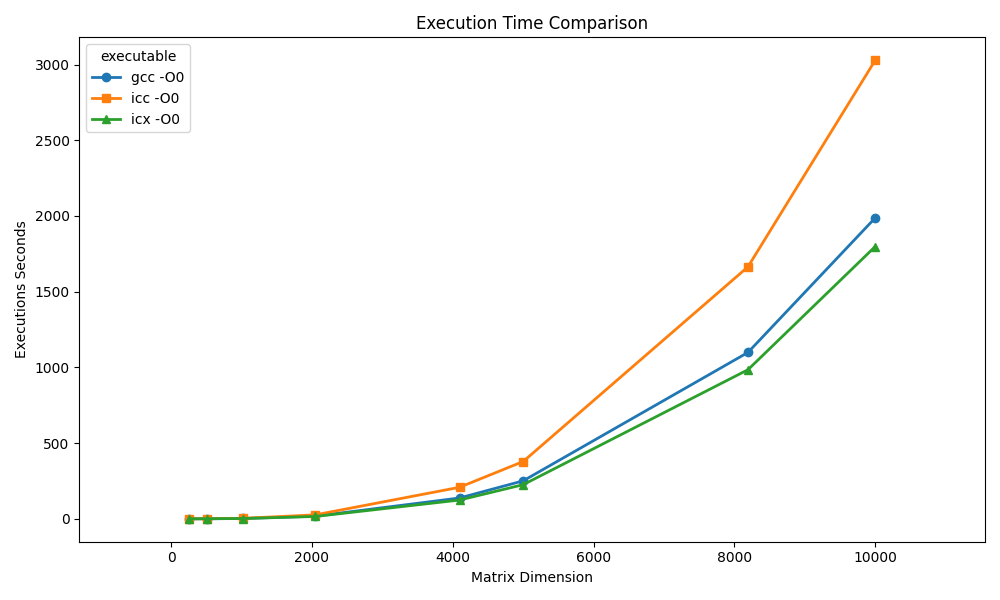
\includegraphics[width=0.6\paperwidth]{Images/all_o0.png}
  }
  \caption{Execution time scaling as a function of matrix size ($n$) at \texttt{-O0}.}
  \label{fig:all_o0}
\end{figure}

\paragraph{Performance Scaling.}
Figure~\ref{fig:all_o0} reports the execution time as a function of matrix size $n$ for the three compilers at \texttt{-O0}. Across all tested input sizes, the scaling behavior strictly follows the expected cubic trend $\mathcal{O}(n^3)$, confirming the theoretical complexity of the algorithm. At this level performance is severely limited, and significant discrepancies observed among the compilers, are not interesting to address, since the generated machine code is a literal, unoptimized translation of the source code.


\paragraph{Intel Advisor and Roofline Analysis.}

The Roofline model (Figure~\ref{fig:icc_o0_roofline}) places the kernel at an extremely low arithmetic intensity ($\approx 0.014$ FLOP/Byte) with a measured performance of merely \textbf{0.66 GFLOPS}. 
Crucially, Advisor indicates that the execution is bottlenecked by the \textbf{Integer Scalar Add Peak} rather than floating-point throughput or memory bandwidth.

\begin{figure}[H]
\centering
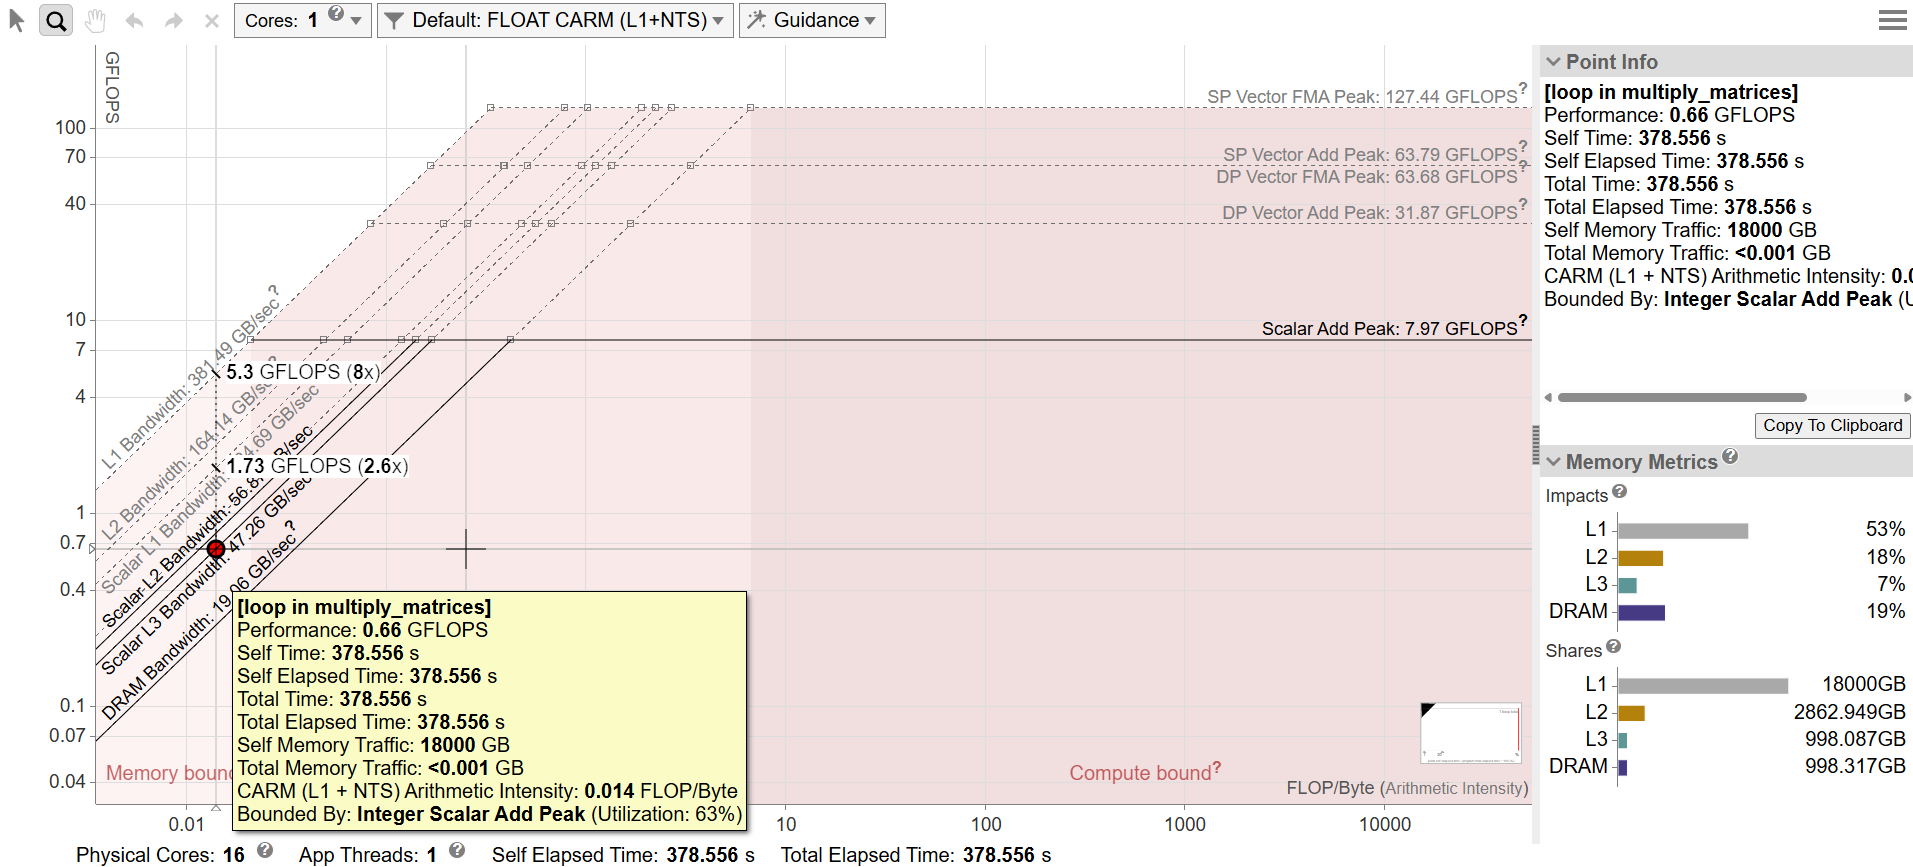
\includegraphics[width=1\textwidth]{Images/icc_o0_roofline.png}
\caption{Intel Advisor Roofline analysis for ICC \texttt{-O0}.}
\label{fig:icc_o0_roofline}
\end{figure}

This massive integer overhead is a direct consequence of the address calculation required for every 2D array access\footnote{The standard 2D array syntax implicitly expands the logical coordinates \texttt{A[i][j]} into a offset \texttt{A[i * n + j]}, requiring a scalar integer multiplication and addition for every single element accessed.}.

Under \texttt{-O0}, the compiler does not perform common subexpression elimination, strength reduction, or loop-invariant code motion. Consequently, these redundant index multiplications and additions are re-evaluated during every single iteration of the innermost loop. Furthermore, the strict lack of register allocation forces the CPU to continuously spill and reload these intermediate address calculations to and from the L1 cache, completely stalling the floating-point pipelines\footnote{This it the main cause of the slow-down, as confirmed by the extremely high number of requests to the L1 cache.}.


\paragraph{Valgrind Cachegrind Analysis.}
The excessive memory traffic caused by the lack of register reuse is confirmed by Valgrind (Figure~\ref{tab:cachegrind_results_o0}). 

\begin{table}[H]
\centering
\caption{Key Valgrind Cachegrind memory profiling metrics for ICC \texttt{-O0}.}
\label{tab:cachegrind_results_o0}
\begin{tabular}{lr}
\toprule
\textbf{Metric} & \textbf{Total Count / Rate} \\
\midrule
Instruction References (I) & \textbf{6,626,402,614,521} \\
Data References (D)        & \textbf{3,000,701,173,012} \\
\midrule
L1 Data Misses             & 31,287,508,170 \\
L1 Data Miss Rate          & 1.0\% \\
\midrule
Last-Level (LL) Misses     & 15,640,639,539 \\
Last-Level (LL) Miss Rate  & 0.2\% \\
\bottomrule
\end{tabular}
\end{table}

The profiling reports approximately 6.6 trillion executed instructions (I refs) alongside 3 trillion data references (D refs). This ratio of roughly 2.2 instructions per data access reflects the massive scalar overhead required simply for loop control and address calculation. 

Despite an enormous cumulative memory traffic footprint ($\approx 18$ TB of L1 interactions), the actual cache miss rates remain relatively low (1.0\% for L1 data, 0.2\% for Last-Level Cache). This confirms that the kernel is not DRAM bandwidth-bound, but rather instruction-bound due to scalar execution.


\paragraph{Compiler Report.}
Finally, the compiler optimization report for \texttt{-O0} confirms the absence of any code transformations. No SIMD instructions are generated (the code relies exclusively on standard scalar x86 instructions), and the nested loops are left entirely intact without unrolling, blocking, or interchange, leading to the severe underutilization of the CPU's computational resources observed in the profiling tools.

%==============================
%-------------O1---------------
%==============================
\subsubsection{Minimal Optimizations (\texttt{-O1})}

The \texttt{-O1} optimization level represents the first step beyond baseline execution, implementing several impacting changes as shown in Figure~\ref{fig:all_o1}.

\begin{figure}[H]
  \centering
  \noindent
  \makebox[0pt][c]{
    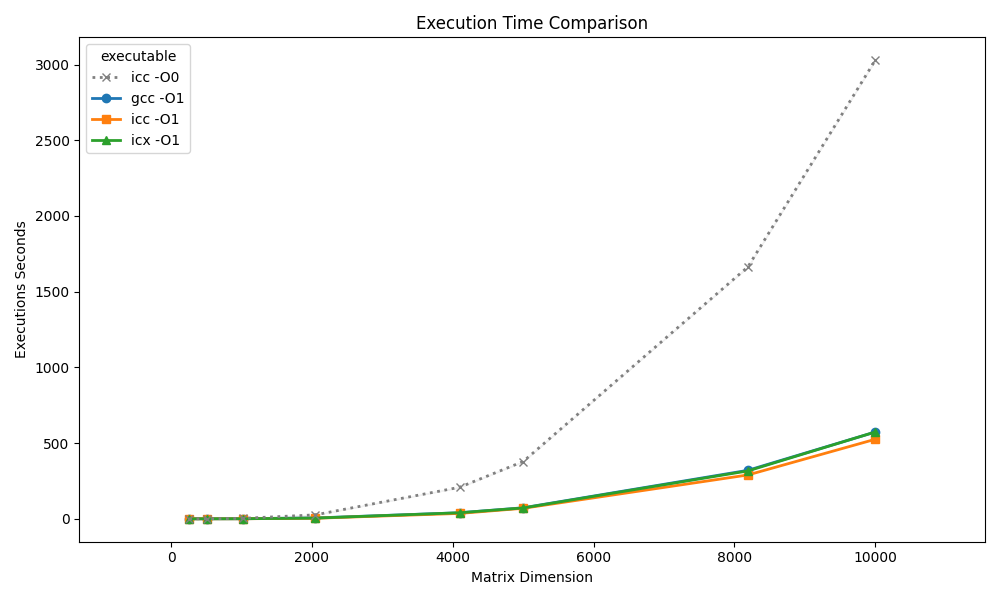
\includegraphics[width=0.6\paperwidth]{Images/all_o1.png}
  }
  \caption{Execution time scaling as a function of matrix size ($n$) at \texttt{-O1}.}
  \label{fig:all_o1}
\end{figure}

At this stage, the compiler enables basic scalar optimizations such as constant folding, dead code elimination, and limited inlining. However, aggressive loop transformations, cache blocking, and automatic vectorization remain inactive. 

The compiler optimization report confirms this behavior, repeatedly issuing the remark: 

\begin{quote}
    \texttt{remark \#15320: routine skipped: loop optimizations disabled}
\end{quote}

This indicates that loop-level optimizations and vectorization passes are not applied under the \texttt{-O1} profile. Consequently, the triple-nested loop is executed in scalar form, failing to exploit the AVX2 SIMD units available on the target architecture. 

Furthermore, the absence of loop restructuring prevents the compiler from improving data locality, leaving the implementation unable to effectively utilize the hardware's caching capabilities.

\paragraph{Intel Advisor Analysis.} 
The Intel Advisor Roofline analysis (Figure~\ref{fig:roofline_o1}) places the kernel in a strictly memory-bound regime. 

\begin{figure}[H]
    \centering
    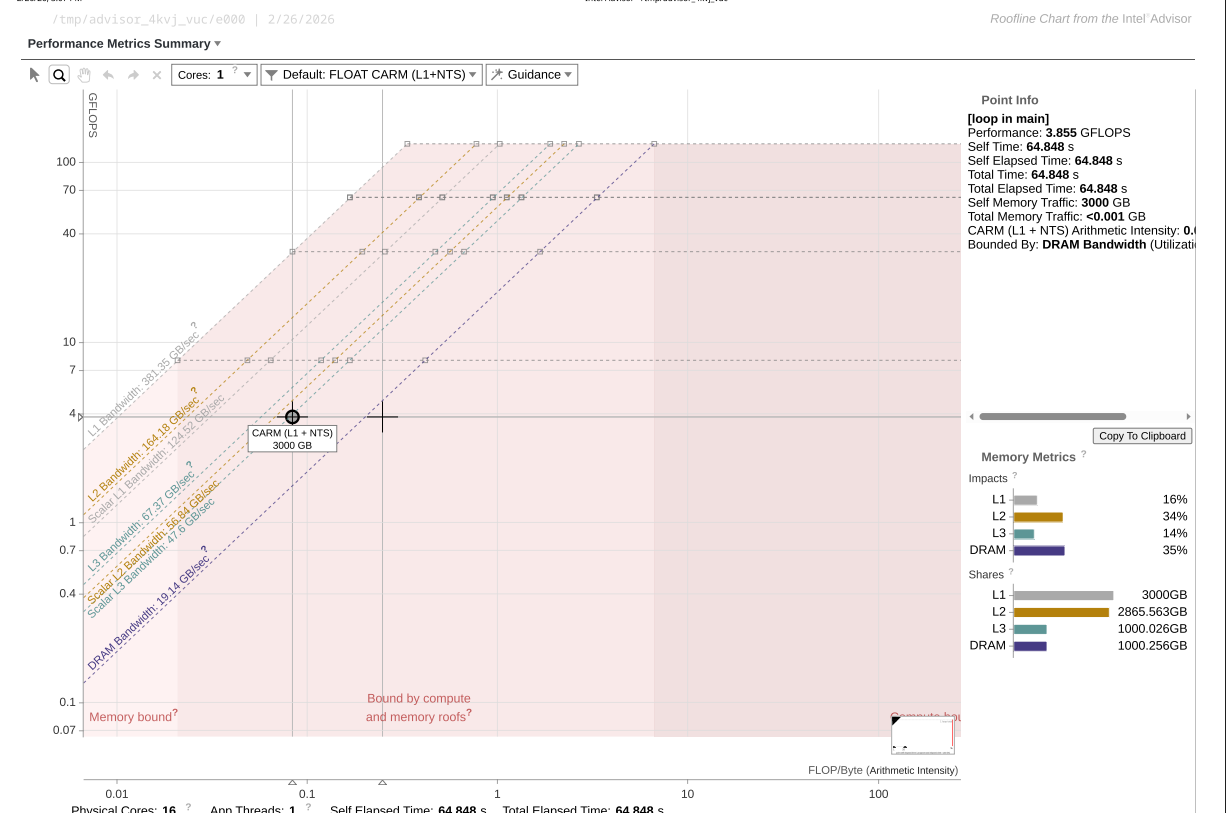
\includegraphics[width=1\textwidth]{Images/icc_o1_roofline.png}
    \caption{Intel Advisor Roofline analysis for ICC \texttt{-O1}.}
    \label{fig:roofline_o1}
\end{figure}

Measured performance reaches \textbf{3.855 GFLOPS}, with an arithmetic intensity of approximately 0.1 FLOP/Byte. Such low intensity indicates that the algorithm performs very few floating-point operations per byte transferred from memory. Execution is thus constrained by memory bandwidth rather than computational throughput, preventing the functional units from reaching their theoretical peak.

The memory hierarchy breakdown further clarifies these performance limitations:

\begin{itemize}
    \item \textbf{Stall Impact:} The dominant stall sources are DRAM (35\%) and L2 (34\%), accounting for nearly 70\% of total execution stalls. This confirms that latency at lower cache levels and main memory significantly limits pipeline utilization.
    \item \textbf{Traffic Distribution:} Memory traffic analysis reports approximately \textbf{3000 GB} of data passing through L1, with the majority propagating to L2 (2865 GB), and nearly 1000 GB reaching L3 and DRAM. This indicates insufficient temporal locality and poor cache residency of the working set.
\end{itemize}

\paragraph{valgrind insight}
Dynamic analysis via Valgrind further corroborates the memory-bound diagnosis. The key metrics for this configuration are summarized in Table~\ref{tab:cachegrind_results_o1}.

\begin{table}[H]
\centering
\caption{Key Valgrind Cachegrind memory profiling metrics for ICC \texttt{-O1} ($n=5000$).}
\label{tab:cachegrind_results_o1}
\begin{tabular}{lr}
\toprule
\textbf{Metric} & \textbf{Total Count / Rate} \\
\midrule
Instruction References (I) & 875,303,318,749 \\
Data References (D)        & 375,101,183,650 \\
\midrule
L1 Data Misses             & 31,309,389,456 \\
L1 Data Miss Rate          & 8.3\% (\textbf{12.5\% Read}) \\
\midrule
Last-Level (LL) Misses     & \textbf{15,640,645,313} \\
Last-Level (LL) Miss Rate  & 1.3\% (6.3\% Read) \\
\bottomrule
\end{tabular}
\end{table}


The L1 data cache exhibits a 12.5\% read miss rate, which is unusually high for high-performance workloads and indicates limited spatial locality within the innermost loop. 
The last-level cache (L3) shows a 6.3\% read miss rate, translating into approximately 15.6 billion accesses to main memory.

Although the overall LL miss rate (1.3\%) appears moderate, the extremely large number of total memory references amplifies the impact of each miss, resulting in substantial DRAM traffic and high latency penalties.

These findings are consistent with the Roofline model and confirm that memory latency and bandwidth represent the primary bottleneck under minimal optimization settings.

\paragraph{Conclusions. }
In summary, the \texttt{-O1} configuration introduces basic scalar optimizations but does not alter the algorithm's fundamental memory access pattern: the combined evidence identifies the kernel as \textbf{bandwidth-bound}.

The triple nested loop remains non-vectorized and untiled, leading to low arithmetic intensity and excessive off-chip memory traffic.



%==============================
%-------------O2---------------
%==============================
\subsubsection{Standard Optimizations (\texttt{-O2})}
The adoption of the \texttt{-O2} optimization level leads to a moderate improvement in performance: at this level, the compiler applies \emph{conservative} optimizations that improve execution speed without "risking" changes to the program's numerical semantics or architectural meaning, such as \textbf{basic auto-vectorization}.

\begin{figure}[H]
\centering
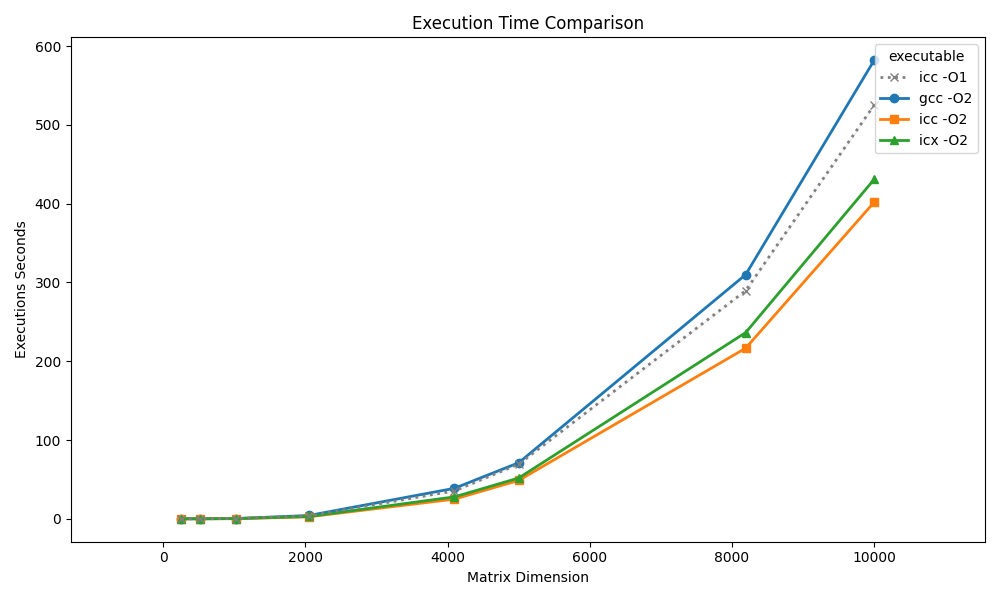
\includegraphics[width=0.8\textwidth]{Images/all_o2.png}
\caption{All compilers -O2 performances compared to ICC -O1}
\label{fig:all_o2}
\end{figure}


\paragraph{Roofline model}
The Roofline model showin in Figure~\ref{fig:icc_o2_roofline} indicates that the working point shifts vertically compared to the \texttt{-O0} configuration, reflecting increased computational throughput at similar arithmetic intensity.
Measured throughput increases to \textbf{6.062 GFLOPS}, corresponding to a 31\% improvement over the previous configuration, and execution time decreases to 49.39 seconds. 

\begin{figure}[H]
\centering
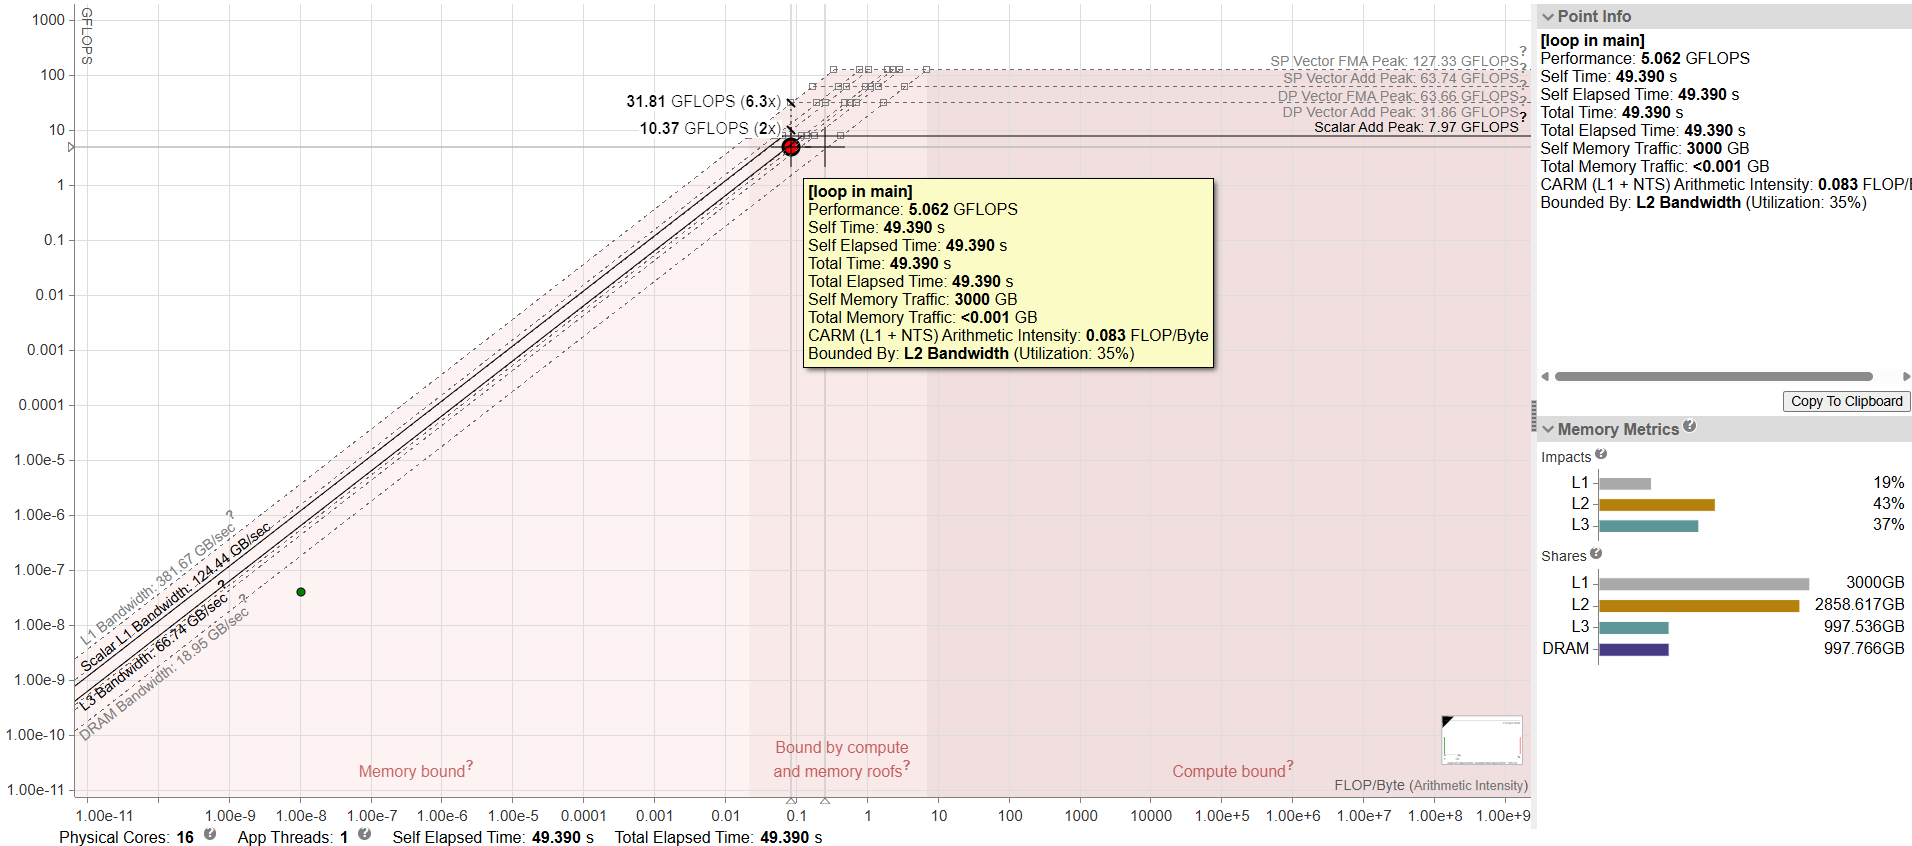
\includegraphics[width=\textwidth]{Images/icc_o2_roofline.png}
\caption{Roofline analysis for ICC -O2.}
\label{fig:icc_o2_roofline}
\end{figure}

The kernel is now bounded by L2 cache bandwidth, as explicitly reported by Advisor (``Bounded by: L2 Bandwidth''). 
This transition suggests that instruction-level inefficiencies have been partially mitigated and that the memory hierarchy has become the dominant constraint.
\paragraph{Valgrind Cachegrind Analysis.}
Dynamic analysis confirms a massive reduction in instruction overhead, though memory pressure has intensified. Key metrics are summarized in Table~\ref{tab:cachegrind_results_o2}.

\begin{table}[H]
\centering
\caption{Key Valgrind Cachegrind metrics for ICC \texttt{-O2}.}
\label{tab:cachegrind_results_o2}
\begin{tabular}{lr}
\toprule
\textbf{Metric} & \textbf{Total Count / Rate} \\
\midrule
Instruction References (I) & 297,143,584,210 \\
Data References (D)        & 187,582,341,902 \\
\midrule
L1 Data Miss Rate          & 16.7\% (25.0\% Read) \\
Last-Level (LL) Miss Rate  & 3.2\% \\
\bottomrule
\end{tabular}
\end{table}

Compared to \texttt{-O1}, the total instruction count fell by nearly 65\% (from 875B to 297B), confirming the efficacy of vectorization. However, the L1 read miss rate has spiked to 25\%. 

This occurs because the faster execution units demand data more aggressively, exposing the locality limitations of the naive $i-k-j$ pattern: the working set exceeds L2 capacity, forcing the stalls observed in the Roofline model.

\newpage
\paragraph{Compiler Report.}
The ICC optimization report confirms that the compiler successfully auto-vectorized the innermost loop, though it utilized a conservative SIMD width.

\begin{lstlisting}[style=CStyle, caption={Simplified ICC Optimization Report for \texttt{-O2}.}]
LOOP BEGIN (i-loop)
    remark #15542: loop was not vectorized: inner loop already vectorized
    LOOP BEGIN (k-loop)
        remark #15542: loop was not vectorized: inner loop already vectorized
        LOOP BEGIN (j-loop)
            remark #15388: aligned access for matrix[i][j] and matrix[k][j]
            remark #15305: vector length 2
            remark #15399: unroll factor set to 4
            remark #15300: LOOP WAS VECTORIZED
        LOOP END
        LOOP BEGIN (j-remainder)
            remark #15335: remainder loop was not vectorized
        LOOP END
    LOOP END
LOOP END
\end{lstlisting}

The report highlights a vector length of 2, indicating \texttt{\textbf{128-bit SIMD}} usage for double-precision operands. This suggests that the compiler is not yet targeting the full 256-bit register's width available on the studied AVX-capable hardware\footnote{The use of 128-bit SIMD instead of 256-bit is a symptom of the code not being fully tuned for the specific target architecture at this optimization level.}. 

Despite this, the unroll factor of 4 and aligned accesses successfully reduced loop-control overhead.


%==============================
%-------------O3---------------
%==============================
\subsubsection{Aggressive Optimizations (\texttt{-O3})}\label{subsec:seq_3}

The adoption of the \texttt{-O3} optimization level produces a dramatic shift in the performance profile of the kernel. At this stage, the compiler goes beyond conservative instruction scheduling and actively restructures the execution pattern to overcome the severe bandwidth bottlenecks caused by poor cache utilization.

\begin{figure}[H]
\centering
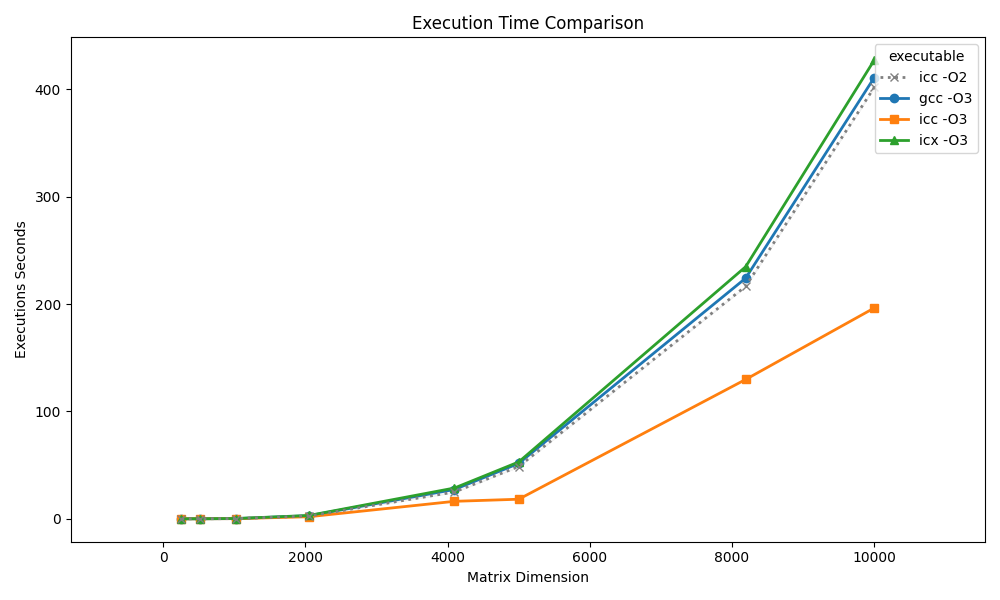
\includegraphics[width=0.8\textwidth]{Images/all_o3.png}
\caption{All compilers -O3 performances compared to ICC -O2}
\label{fig:all_o3}
\end{figure}


\paragraph{Compiler Optimization Report}
The ICC optimization report reveals that the compiler has fundamentally refactored the triple-nested loop into a complex, multi-level structure\footnote{See Appendix~\ref{subsec:tiling} for an in-depth explanation of how the \emph{Tiling Algorithm} works.}.

\begin{lstlisting}[style=CStyle, caption={Refactored ICC Optimization Report for \texttt{-O3}.}]
LOOP BEGIN (i-tile)
    LOOP BEGIN (k-tile)
        LOOP BEGIN (j-tile)
            LOOP BEGIN (i-inner) blocked by 128
                LOOP BEGIN (k-inner) blocked by 128
                    1. LOOP BEGIN (j-peeled)
                    2. LOOP BEGIN (j-vectorized)
                         remark #15388: aligned access
                         remark #15305: vector length 2, unroll factor 4
                         remark #15300: LOOP WAS VECTORIZED
                    3. LOOP BEGIN (j-alternate-alignment)
                    4. LOOP BEGIN (j-remainder)
                         remark #15335: loop not vectorize
                LOOP END
            LOOP END
        LOOP END
    LOOP END
LOOP END
\end{lstlisting}


\paragraph{Intel Advisor Roofline Analysis}
The structural changes translate directly into a massive throughput increase, as shown in the Roofline model (Figure~\ref{fig:icc_O3_roofline}).

\begin{figure}[H]
\centering
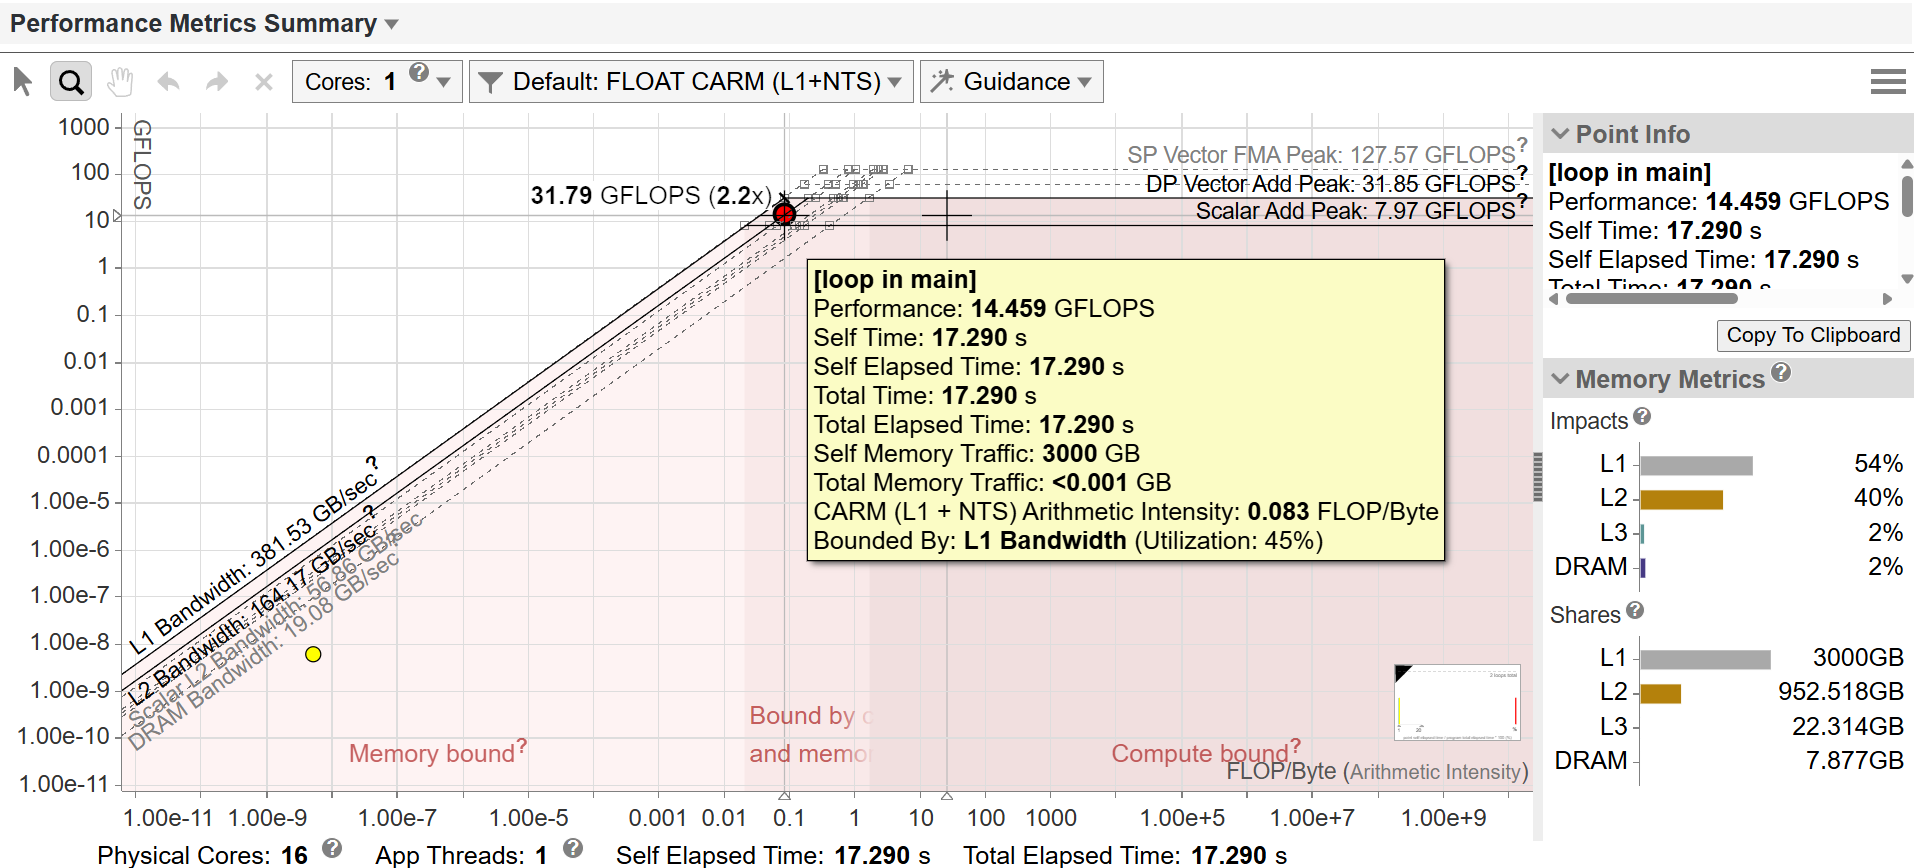
\includegraphics[width=\textwidth]{Images/ICC_O3_Roofline.png}
\caption{Roofline analysis for ICC \texttt{-O3}.}
\label{fig:icc_O3_roofline}
\end{figure}

The kernel achieves a computational throughput of \textbf{14.459 GFLOPS}, a significant uplift from \texttt{-O2} (that performed 6.062 GFLOPS). 

Observe how the \textbf{Arithmetic Intensity (AI)} keep the same value as the previous optimization at $0.083$ FLOP/Byte: this confirms that the performance gain is not due to doing "less memory work" per operation, but rather doing that work much faster by shifting the bottleneck.

The kernel's operational point has exceeded the scalar add peak, moving toward the vector add peak; the bottleneck is now  \textbf{L1 Bandwidth Bound} (saturating 45\% of maximum capacity). 

The decomposition of execution time shows that the L1 cache (54\%) and L2 cache (40\%) are the primary bottlenecks, while DRAM impact is negligible. 

This proves the tiling was successful: the data is now almost entirely encapsulated within the smaller (and faster) caches.

\paragraph{Valgrind Cachegrind Analysis}

The efficacy of the tiling is quantitatively confirmed by the memory profiling in Table~\ref{tab:cachegrind_results_o3}.

\begin{table}[H]
\centering
\caption{Key Valgrind Cachegrind metrics for ICC \texttt{-O3}.}
\label{tab:cachegrind_results_o3}
\begin{tabular}{lr}
\toprule
\textbf{Metric} & \textbf{Total Count / Rate} \\
\midrule
Instruction References (I) & 297,143,584,210 \\
Data References (D)        & 187,582,341,902 \\
\midrule
L1 Data Miss Rate          & \textbf{8.9\%} \\
Last-Level (LL) Miss Rate  & \textbf{0.1\%} \\
\bottomrule
\end{tabular}
\end{table}

The L1D miss rate has dropped significantly to 8.9\%, indicating much better temporal locality. Most importantly, the L3 miss rate is near-zero (0.1\%). This demonstrates that despite the large matrix size, the optimized access pattern ensures that almost no data requests need to traverse the hierarchy to the DRAM. The high degree of data reuse within the primary and secondary caches allows the CPU to sustain much higher GFLOPS by avoiding the high-latency penalty of main memory.

%==============================
%-------------O3 xHost (-DALIGN)---------------
%==============================

\subsection{Compiler(s), to the moon: beyond \texttt{-O3}}

Now that we have studied in-depth the behavior of the compiler given the default optimizations \texttt{-O}, we can further drive the compilation towards even more optimized code by giving even more specific flags to the compilers. 

For brevity, we define a set of these flags simultaneously to evaluate their cumulative impact on the kernel's performance, without explicitly define what is their separate impact on the generated assembly.

\begin{table}[H]
\centering
\begin{threeparttable}
\caption{Advanced compiler optimization flags and their expected effects.}
\label{tab:advanced_flags}
\begin{tabular}{lp{3cm}p{7cm}}
\toprule
\textbf{Flag} & \textbf{Category} & \textbf{Microarchitectural Effect} \\
\midrule
\texttt{-xHost} & Architecture & Instructs the compiler to target the highest instruction set available on the local host\tnote{1}, enabling the widest possible SIMD registers. \\
\midrule
\texttt{-fp-model fast=2} & Floating Point & Enables aggressive floating-point optimizations. It allows for reordering of operations and ignores strict IEEE 754 rules to maximize throughput\tnote{2}. \\
\midrule
\texttt{-fno-alias} & Memory & Asserts that no two pointers point to the same memory location, allowing the compiler to reorder loads and stores without "aliasing" checks. \\
\midrule
\texttt{-inline-level=2} & Inlining & Increases the intensity of function inlining to replace function calls with the actual function body, reducing branch penalties and call overhead. \\
\midrule
\texttt{-unroll-aggressive} & Loop Control & Enables aggressive loop unrolling heuristics, attempting to unroll loops even when the benefit is not immediately obvious to standard logic. \\
\midrule
\texttt{-unroll=4} & Loop Control & Specifically sets the unroll factor to 4, ensuring four iterations are processed as a single block to reduce loop-counter overhead. \\
\bottomrule
\end{tabular}

\begin{tablenotes}
    \footnotesize % This makes the font smaller
    \item[1] \textbf{AVX2} on the tested workstation, as reported in Table~\ref{tab:cpu_specs}.
    \item[2] For this reason, at test time the results of the kernel are explicitly checked to ensure results do not differ from the correct behavior.
\end{tablenotes}
\end{threeparttable}
\end{table}
\paragraph{Refactored Optimization Report.}
The following report summarizes the complex loop transformation strategy achieved with these aggressive flags.


The improvements with respect to the previous iteration are noticeable:

\begin{itemize}
    \item \textbf{Array Refs Replacement:} The compiler avoid the iterative request to obtain \texttt{C[i][j]} at each iteration, and decide to save its value in a register for a way-faster access.

    \item \textbf{Vectorization Width:} While standard \texttt{-O3} utilized a conservative vector length of 2 (128-bit), the addition of \texttt{-xHost} enables \textbf{vector length 4}.
    \item \textbf{Unroll and Jam:} The compiler now implements "Unroll and Jam" by a factor of 4. This technique unrolls the outer loops of a nest and fuses the resulting bodies, which significantly improves register reuse and ensure  a better use of the caches hierarchy\footnote{The exact steps implemented, along with the motivations, are explained in Appendix~\ref{subsec:unroll_jam}.}.
    \item \textbf{Vectorized Remainders:} The compiler now successfully \textbf{vectorizes the remainder loops}. This ensures that performance does not drop sharply at the boundaries of the matrix tiles.
\end{itemize}

\newpage
\begin{lstlisting}[style=CStyle, caption={Simplified ICC Report:\texttt{-O3 -xHost}.}]
LOOP BEGIN (i - tile )
    LOOP BEGIN (k - tile )
        LOOP BEGIN (j - tile )
            remark #25440: unrolled and jammed by 4 (pre-vector)    
            LOOP BEGIN (i - inner ) blocked by 128
                LOOP BEGIN (k - inner ) blocked by 128
                    LOOP BEGIN (j-vectorized) blocked by 128
                        remark #15289: vectorization support: unaligned access 
                        remark #15295: vectorization support: vector length 4
                        remark #15297: vectorization support: unroll factor set to 4
                        remark #15298: LOOP WAS VECTORIZED
                        remark #15300: Number of Array Refs Scalar Replaced In Loop
                    LOOP END
                    LOOP BEGIN (j-remainder)
                        remark #15301: REMAINDER LOOP WAS VECTORIZED
                        remark #15302: Number of Array Refs Scalar Replaced In Loop
                    LOOP END
                LOOP END
            LOOP END
        LOOP END
    LOOP END
LOOP END
\end{lstlisting}


\paragraph{Intel Advisor Roofline Analysis}

The impact of the \texttt{-xHost} flag is clearly visible in the transition to AVX2 execution. The kernel now achieves a computational throughput of \textbf{29.463 GFLOPS}. This is approximately double the performance of the standard \texttt{-O3} configuration, which reached 14.459 GFLOPS.

\begin{figure}[H]
\centering
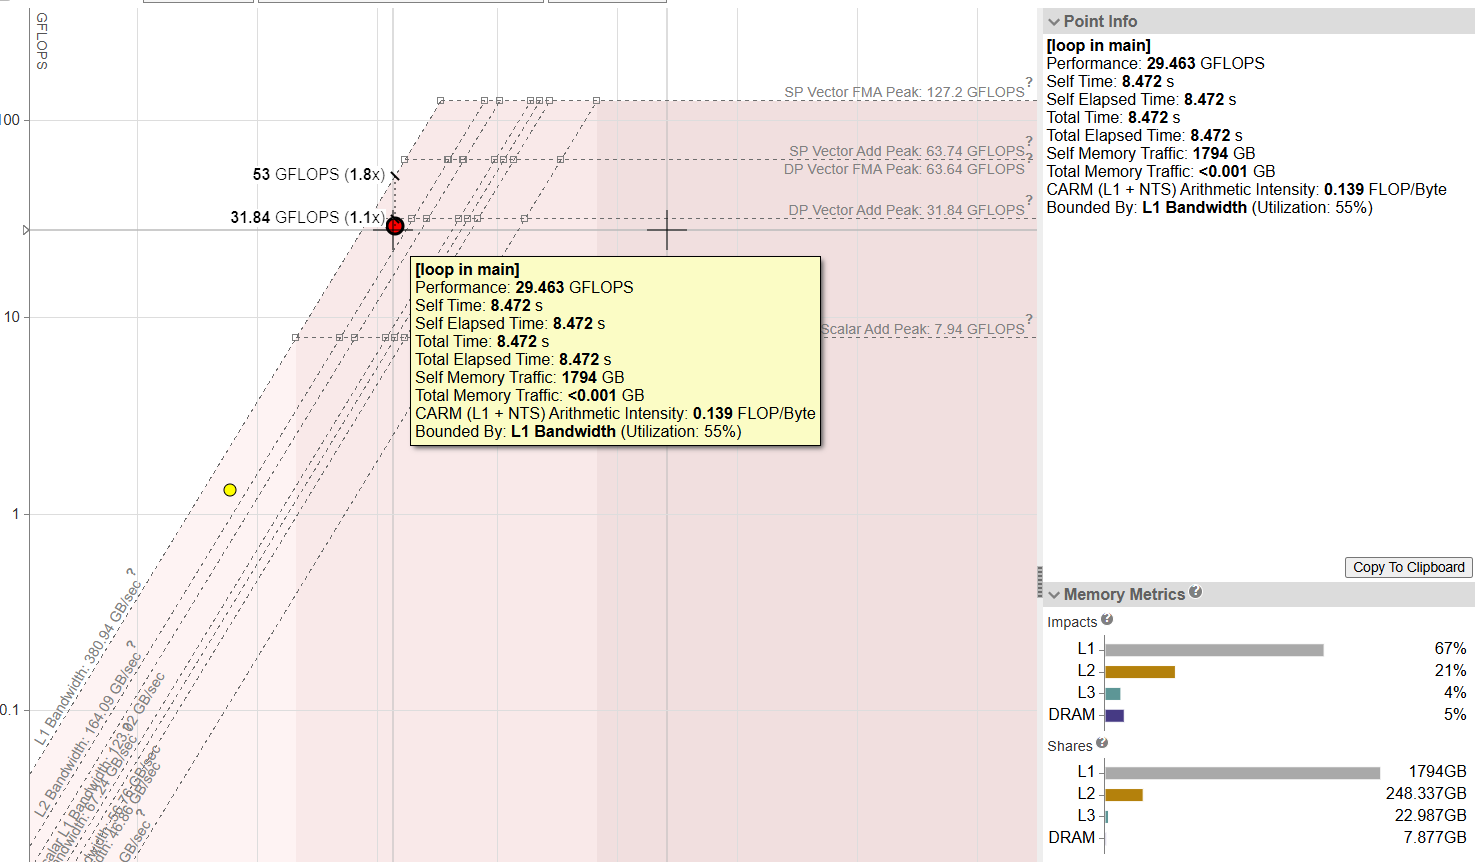
\includegraphics[width=1\textwidth]{Images/icc_better_roofline.png}
\caption{Roofline analysis for ICC \texttt{-O3 -Xhost etc...}.}
\label{fig:icc_better_roofline}
\end{figure}

The operational point on the Roofline model confirms this architectural shift, as the kernel now sits just under the DP Vector Add Peak (31.84 GFLOPS).

\paragraph{Performance comparison}

Lastly, we compare the performance of ICC against ICX\footnote{The ICX report indicates the same optimizations, with the exception that block sizes are $64 \times 64 \times 64$, whereas ICC utilizes $128 \times 128 \times 128$.} across a significantly broader domain of matrix sizes.

\begin{figure}[H]
\centering
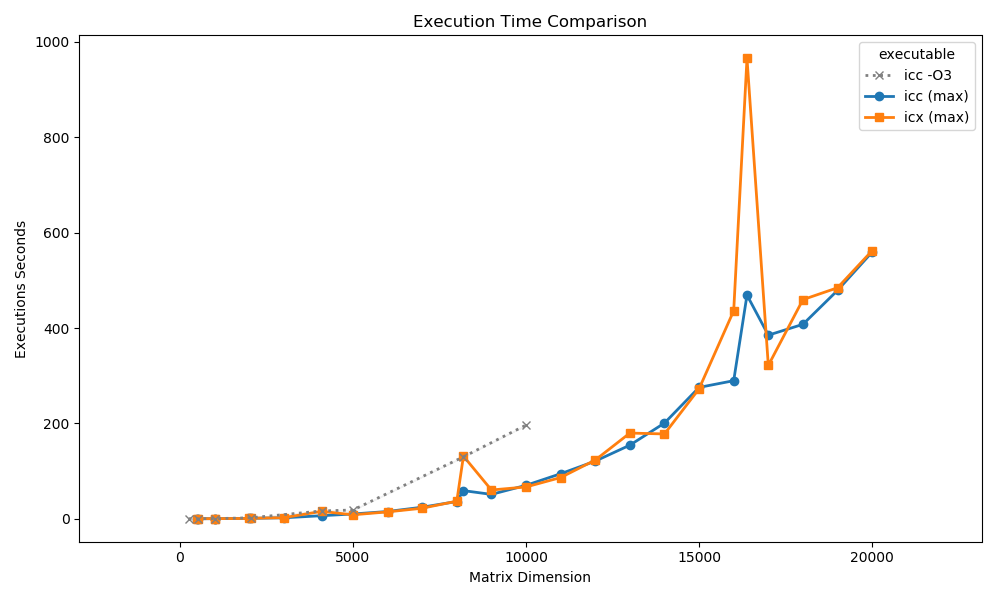
\includegraphics[width=0.8\textwidth]{Images/icc_icx_max.png}
\caption{Performance comparison of ICC and ICX with the advanced flags.}
\label{fig:icc_icx_better_comparison}
\end{figure}

It is immediately apparent that both highly optimized executables suffer a significant performance degradation when the matrix dimension $n$ is a power of 2 (e.g.,$n=4096$, $n=8192$, $n=16384$). 
In contrast, performance remains consistently high and scales more predictably when $n$ does not align with these boundaries.
This specific bottleneck is well motivated in the in-depth explanation in Appendix~\ref{subsec:caching}.

Nonetheless, we will also attempt once again to obtain another improvement: as noted in the optimization report, the main loop body still notify unaligned accesses, which limits the efficiency of the SIMD operations.

\subsubsection{A little price to pay for salvation? \texttt{-DALIGN}}
Note that a standard cache line is 64 bytes, which perfectly accommodates 8 double-precision (8-byte) values. 
When the matrix dimension $n$ (in particular the row's lenght) is not a multiple of 8, the compiler must generate "peeled" and "remainder" loops to handle those edge cases\footnote{Misalignment can also occur if the starting memory address is not aligned with the cache line boundary, but this is easily avoided by calling \texttt{posix\_memalign(ptr, 64, tot\_bytes)} at runtime.}.

By enabling the \texttt{-DALIGN} flag, we explicitly augment the matrix size from $n \times n$ to $n' \times n'$, where $n'$ is the smallest multiple of 8 greater than or equal to $n$.


The "overflow" cells in this padding area are initialized to zero to ensure they do not affect the mathematical results of the matrix multiplication (as explained in Appendix~\ref{subsec:padding}).

\paragraph{Practical Advantages.}

This approach, \textbf{while requiring slightly more memory}, provides several advantages:

\begin{itemize}
\item \textbf{Cache Line Alignment:} 
It is explicitly ensured by the code itself, without relying on the compiler's optimizations.

\item \textbf{Loop Simplification:} Because every row is now also a multiple of the register's capacity (4 doubles), the compiler no longer needs to generate auxiliary loops.

\item \textbf{SIMD Efficiency:} The hardware can perform 256-bit loads and stores at peak speed, as there is no longer a risk of a single vector instruction spanning across two different cache lines (nor incomplete register, that must be explicitly masked with zeros).
\end{itemize}


\paragraph{Compilation report}
The report produced by ICC clearly show a shortened, simplified version of the previous iteration\footnote{The  report from ICX showed once again how the only difference was in the choice of the block size, as before $64 \times 64 \times 64$.}.


\begin{lstlisting}[style=CStyle, caption={Optimization report of ICC with \texttt{-O3 -xHost -DALIGN}.}]
LOOP BEGIN (i-tile)
    LOOP BEGIN (k-tile)
        LOOP BEGIN (j-tile)
            remark #25440: unrolled and jammed by 4 (pre-vector)    
            LOOP BEGIN (i-inner) blocked by 125
                LOOP BEGIN (k-inner) blocked by 125
                    LOOP BEGIN (j-vectorized) blocked by 128
                        remark #15388: vectorization support: reference C[i][j] has aligned access
                        remark #15388: vectorization support: reference B[k][j] has aligned access
                        remark #15305: vectorization support: vector length 4
                        remark #15399: vectorization support: unroll factor set to 4
                        remark #15300: LOOP WAS VECTORIZED
                    LOOP END
                    LOOP BEGIN (j - remainder )
                        remark #15301: REMAINDER LOOP WAS VECTORIZED
                    LOOP END
                LOOP END
            LOOP END
        LOOP END
    LOOP END
LOOP END
\end{lstlisting}

\paragraph{Performance}

Figure~\ref{fig:icc_icx_aligned_comparison} demonstrates that even if \texttt{-DALIGN} successfully lowers execution times, matrices with dimensions power-of-two (and neighboring values) remain a major bottleneck.

\begin{figure}[H]
\centering
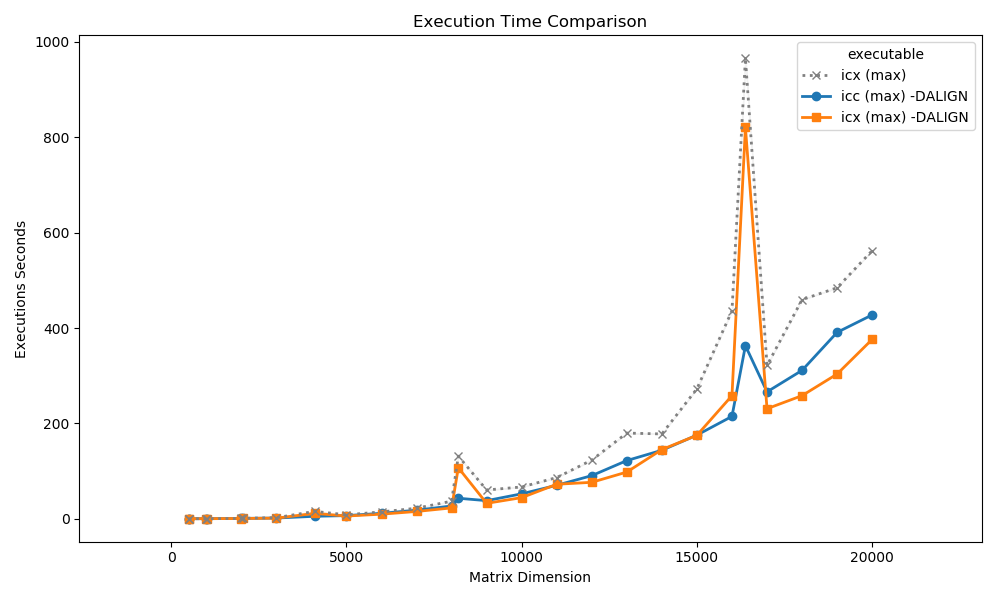
\includegraphics[width=0.8\textwidth]{Images/icc_icx_aligned.png}
\caption{Performance comparison of ICC and ICX with the advanced flags and -DALIGN.}
\label{fig:icc_icx_aligned_comparison}
\end{figure}

ICX achieves the best overall performance in standard cases but suffers the most extreme penalties at problematic dimensions. In contrast, ICC is slightly slower on average but far more stable, handling worst-case scenarios with much greater consistency.

Now we are equipped to  better understand the problem with those last implementations.


%==============================
%-------------EXPLICIT TILING ---------------
%==============================
\subsection{Compiler's limitation, and how to bypass them}

The compiler’s strategy of partitioning the iteration space into blocks $128 \times 128 \times 128$, supplemented by a 4-way unroll-and-jam transformation, is explicitly engineered to maximize the utilization of the  memory hierarchy. 

With those implementation choices, a single $128 \times 128$ tile of requires 128 KB of memory. While this exceeds the 48 KB L1D cache capacity, the \emph{unroll-and-jam} allow for sub-tiles to stay in L1D, while the full $128 \times 128$ block fits inside the L2 cache (1.25 MB per core). 

However, this hardware-specific optimization counld falls short in practice, due to a fundamental limitation in the cache implementation (Behavioral details of the Associative Caches are discussed in Appendix~\ref{subsec:caching}). 

\subsubsection{Cache Collisions in Matrix Traversal}
For simplicity, we consider an aligned matrix implementation with cache-line padding (i.e., the starting pointer is cache-aligned, and the matrix content is perfectly bounded by cache lines): under those constrains, we can find the worst-case scenario of cache trashing.

When iterating through a matrix column, the CPU accesses addresses separated by the length of an entire matrix row. If this row length in memory exactly matches the distance between \emph{cache sets}, the first element of every row will map to the exact same, causing severe cache thrashing by evicting one of the already-allocated cache lines\footnote{Usually the cache eviction follows a Least-Recently-Used (LRU) replacement policy, hence will be removed the cache line first addressed.}.

For a cache with a power-of-two number of sets, addresses map to the same set if they are separated by exactly $2^{(\text{Set bits} + \text{Offset bits})}$ bytes. For a matrix of double-precision floating-point numbers (\texttt{sizeof(double)} $= 8$ bytes), the required row length to force a collision is:
$$ \text{Row Length} = \frac{2^{(\text{Set bits} + \text{Offset bits})}}{8} \text{ elements} $$

Based on the hardware specifications in Table~\ref{tab:cache_partitioning}, we can calculate the exact matrix dimensions that trigger these set collisions:

\begin{itemize}
    \item \textbf{L1 Cache Collision:} 
    The L1 cache uses 6 Offset bits and 6 Set bits.
    $$ \text{L1 Distance} = 2^{(6 + 6)} = 2^{12} \text{ bytes} = 4096 \text{ bytes} $$
    $$ \text{L1 Row Length} = \frac{4096}{8} = 512 \text{ elements} $$
    If the matrix has exactly 512 columns (or a multiple of it), the first element of every row maps to the same L1 set. Since the L1 is 12-way associative, reading just 13 rows in a column will completely fill the set and force an eviction of the first row (as observed in Figure~\ref{fig:icc_icx_aligned_comparison}).

    \item \textbf{L2 Cache Collision:}
    The L2 cache uses 6 Offset bits and 11 Set bits.
    $$ \text{L2 Distance} = 2^{(11 + 6)} = 2^{17} \text{ bytes} = 131,072 \text{ bytes} $$
    $$ \text{L2 Row Length} = \frac{131072}{8} = 16,384 \text{ elements} $$
    If the matrix has exactly 16,384 columns, column-major traversal will rapidly thrash the 10-way associative L2 cache.
\end{itemize}

\paragraph{Quantitative comparison}
This limitation can be verified by the in-depth study we completed by using Intel Advisor on the same ICX build (\texttt{-O3 -xHost -DALIGN}), testing both $N = 4096$ and $N=5000$.

\begin{figure}[H]
\centering
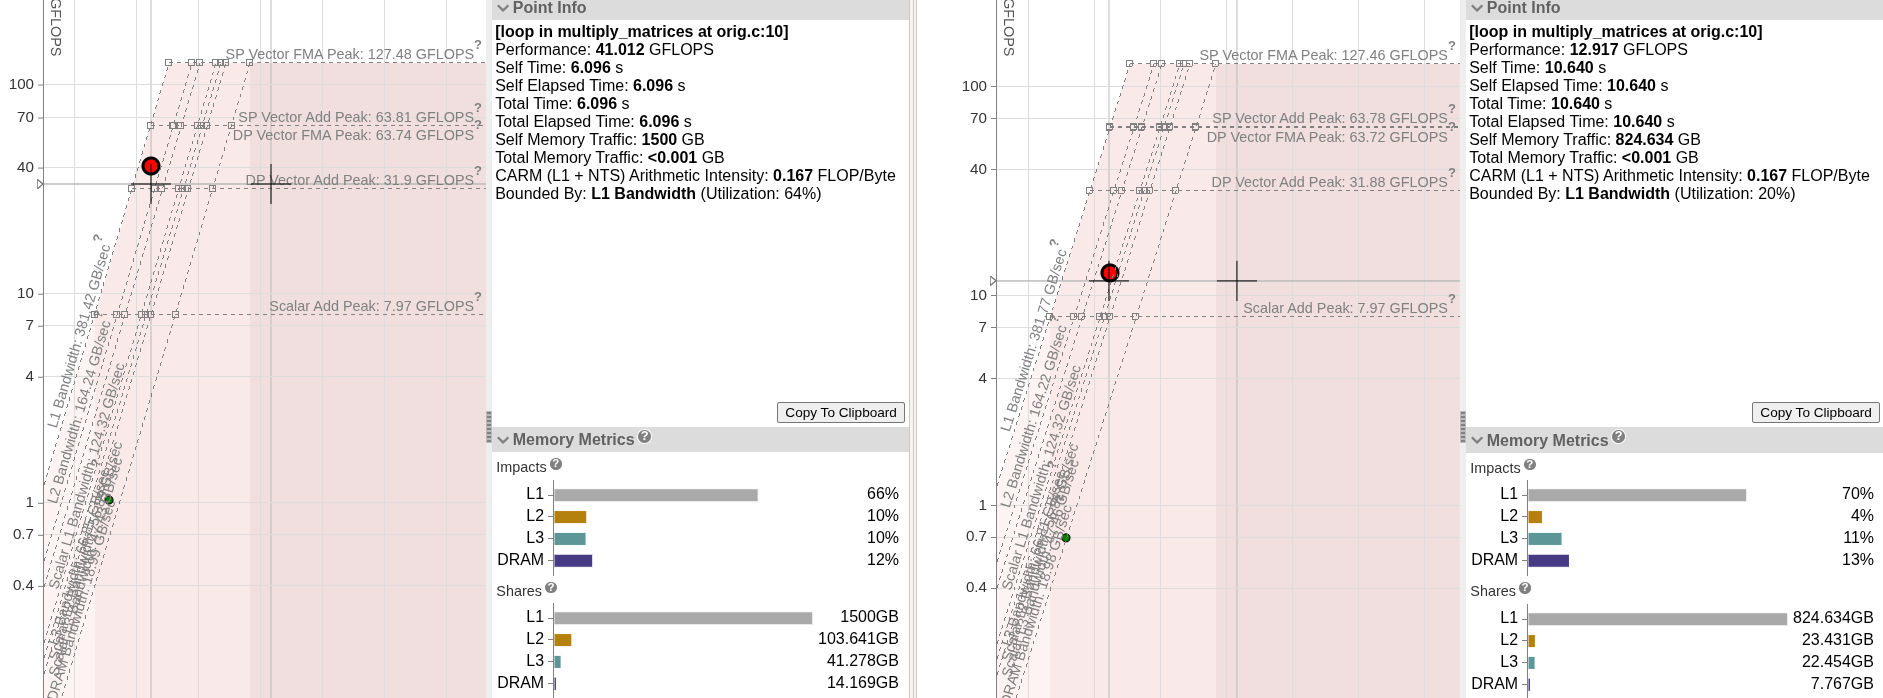
\includegraphics[width=1\textwidth]{Images/icx_4096_vs_5000.png}
\caption{Roofline model of \texttt{ICX -O3 -xHost -DALIGN} on \texttt{n=5000} and \texttt{n=4096}}
\label{fig:icc_icx_aligned_roofline_comparison}
\end{figure}


The highlighted bottlenecks are in both cases the L1, but we can clearly see a difference in their bandwidth utilization and overall performance impact. For the bigger matrix ($N=5000$), the L1 cache is utilized efficiently at 64\% of its peak bandwidth, allowing a performance of \textbf{41.01 GFLOPS}.

In contrast, the problematic one ($N=4096$) suffers a drop  to just \textbf{12.91 GFLOPS}. 

Despite executing fewer total mathematical operations (due to the smaller size), its L1 bandwidth utilization drops to a mere 20\%: this low utilization indicates that the CPU pipeline is heavily stalled waiting for data due to continuous cache conflict evictions (thrashing).



\subsubsection{Cache-Aware Solutions, to Dimension-Dependent Thrashing}

The cache thrashing problem  maximized by power-of-two matrices can be mitigated using three (alternative or complementary) strategies:

\begin{itemize}
    \item \textbf{Memory Padding:} extending each matrix row with a adequate number of cells (zeroed or inaccessible).
    By artificially forcing the row length to a non-power-of-two size\footnote{is possible to compute a runtime a heuristic matrix size that minimize problem, but for brevity purposes we will not explore those solutions.}, the memory addresses are staggered. 
    This naturally shift the column elements across different cache sets rather than concentrating them into the same one. 
    
    We discard this solution because it wastes significant memory space. Furthermore, it assumes we have full control over the original matrices allocations, which is rarely true in real-case scenarios.\footnote{Note that this differs from the minor cache-line alignment padding introduced earlier; padding to break L1 set collisions requires way larger, system-dependent offsets.}

    \item \textbf{Compile-Time Constant Dimensions:} The second solution relies on aggressive compiler optimization. When the matrix dimension $N$ is provided as a constant at compile time, the compiler can further mitigate the effect by using \emph{register blocking} (scalar replacement). Instead of repeatedly fetching conflicting addresses from the L1 cache, the compiler loads the active working set directly into the CPU's vector registers and holds them there throughout the inner loop's execution. 
    
    As shown in Table~\ref{tab:results_placeholder}, the compiler's knowledge partially mitigate the problem, but without completely removing it.

    \begin{table}[H]
    \centering
    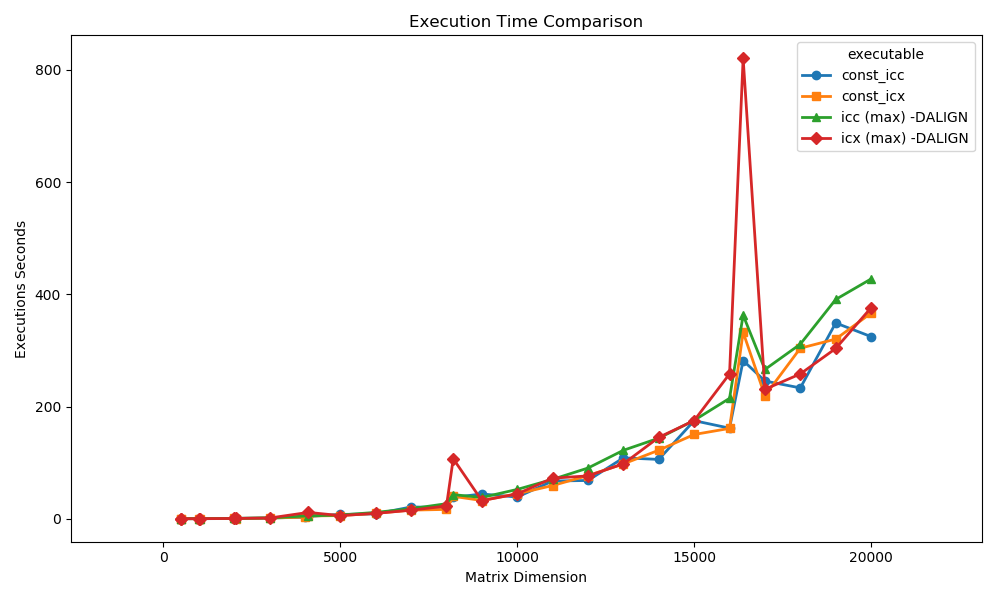
\includegraphics[width=0.8\textwidth]{Images/icc_icx_const.png}
    \caption{Performance comparison demonstrating the furhter dumping of cache thrashing spikes when $N$ is known at compilation time.}
    \label{tab:results_placeholder}
    \end{table}

    \item \textbf{Data Packing (Auxiliary Buffers):} The Last solution proposed is a technique widely employed by high-end optimization libraries such as \texttt{\texttt{OpenBLAS}}, whose detailed breakdown is provided in Appendix~\ref{subsec:openblas}. 
    
    The core idea is to explicitly allocate auxiliary memory buffers and manually copy the active tiles from matrices A and B into these buffers before computing them. Because these temporary matrices are strictly contiguous, they map cleanly across all available cache sets, completely bypassing the original column-stride layout. If implemented correctly and with suitable tile's dimensions, the time used to copy the tiles  will be largely repaid by the performance gains.
\end{itemize}

In the following section, we will present a custom, ad-hoc implementation that applies this packing strategy.


%==============================
%-------------openBlas-like implementation ---------------
%==============================
\subsection{BLAS-like implementation}
Since the attempts to drive the compiler toward the best possible optimization failed, the last chance we have is to explicilty use \texttt{\textbf{AVX intrinsics}} to leverage the CPU's extended registers.

While the low-level implementation motivation are extensively explained in Appendix~\ref{subsec:openblas}, some tinkering with the code was needed to make it work with our use case. 

\subsubsection{Kernel $4\times8$}
In particular, the heart of the  algorithm is the \emph{kernel}, capable to work on multiple cells at the same time; we had to explicitly define it\footnote{In high-end libraries is directly written in Assembly or is written in a source code already "expanded" (i.e. with explicit unrolling, jamming, ...) by scripts that manages all edge-cases and hardware-dependent implementations.}.

\begin{lstlisting}[style=CStyle, caption={Kernel $4\times8$ doubles implementation},label={blas_like_code}]
static inline void kernel_4x8(int n, double (*C)[n], 
                              const double packedA_panel[KC][4], 
                              const double packedB_panel[KC][8], 
                              int kc, int i0, int j0) {
    __m256d c[4][2]; 
    #pragma unroll(4)
    for (int i = 0; i < 4; i++) { // Initialize accumulators
        c[i][0] = _mm256_setzero_pd();
        c[i][1] = _mm256_setzero_pd();
    }
    for (int p = 0; p < kc; p++) { //iterate over kc
        __m256d b0 = _mm256_load_pd(&packedB_panel[p][0]);
        __m256d b1 = _mm256_load_pd(&packedB_panel[p][4]);

        #pragma unroll(4)
        for (int i = 0; i < 4; i++) {
            __m256d a = _mm256_broadcast_sd(&packedA_panel[p][i]);
            c[i][0] = _mm256_fmadd_pd(a, b0, c[i][0]);
            c[i][1] = _mm256_fmadd_pd(a, b1, c[i][1]);
        }
    }
    #pragma unroll(4)
    for (int i = 0; i < 4; i++) {  // Update result matrix C
        __m256d orig0 = _mm256_load_pd(&C[i0 + i][j0 + 0]);
        __m256d orig1 = _mm256_load_pd(&C[i0 + i][j0 + 4]);
        _mm256_store_pd(&C[i0 + i][j0 + 0], _mm256_add_pd(orig0, c[i][0]));
        _mm256_store_pd(&C[i0 + i][j0 + 4], _mm256_add_pd(orig1, c[i][1]));
    }
}
\end{lstlisting}

 It calculates a $4 \times 8$ block of the destination matrix $C$ by multiplying a packed $4 \times kc$ panel of $A$ with a packed $kc \times 8$ panel of $B$. 

\paragraph{Optimization details}
This kernel is designed to fully utilize the capabilities of the AVX2 instruction set, which guarantees \texttt{\textbf{$16 \times$ 256-bit YMM}} registers. 

The kernel at any time keep a $4 \times 2$ array of \texttt{\_\_m256d} vectors. Since each vector holds four double-precision floating-point numbers, the 8 registers stores the 32 elements of the $4 \times 8$ target block of $C$.

By keeping the 8 accumulator registers, 2 registers for $B$, and 1 register for $A$ strictly in the CPU hardware, this kernel uses exactly 11 out of the 16 available \texttt{YMM} registers. This deliberate $4 \times 8$ sizing guarantees that all intermediate calculations occur without any costly "register spilling" to the L1 cache. 

After the iteration along the hidden dimension kc, the accumulated results are loaded, added to the original unaligned $C$ memory locations, and written back.

\paragraph{AVX Intrinsics Reference}
To achieve this low-level control, the kernel relies on Intel Intrinsic functions, which map directly to specific assembly instructions.

\begin{table}[H]
\centering
\caption{AVX2 Intrinsics used in the $4 \times 8$ kernel.}
\label{tab:avx_intrinsics}
\begin{tabular}{lp{10cm}}
\toprule
\textbf{Intrinsic Function} & \textbf{Hardware Operation} \\
\midrule
\texttt{\_\_m256d} & The underlying data type representing a 256-bit \texttt{YMM} register, that can holds 4 double-precision numbers. \\
\midrule
\texttt{\_mm256\_setzero\_pd()} & Returns a 256-bit vector with all bits set to zero.\\
\midrule
\texttt{\_mm256\_load\_pd(ptr)} & Loads 4 packed double-precision values from memory into a vector.\\
\midrule
\texttt{\_mm256\_broadcast\_sd(ptr)} & Loads a single double-precision value from memory and duplicates (broadcasts) it across all 4 elements of the destination vector. \\
\midrule
\texttt{\_mm256\_fmadd\_pd(a, b, c)} & Performs a Fused Multiply-Add operation. It computes $(a \times b) + c$ for all 4 packed elements simultaneously, maintaining infinite intermediate precision before rounding. \\
\midrule
\texttt{\_mm256\_add\_pd(a, b)} & Performs a standard element-wise addition of two 256-bit vectors containing double-precision values. \\
\midrule
\texttt{\_mm256\_storeu\_pd(ptr, a)} & Stores 4 double-precision values from a vector into a  memory location.\\
\bottomrule
\end{tabular}
\end{table}

\paragraph{Hyperparameter tuning}
The algorithm requires tuning the tiling dimensions \texttt{\textbf{MC, NC}}, and \texttt{\textbf{KC}}. The static kernel size ($N_R = 8$, $M_R = 4$), along with the simplification implemented imposes strict alignment constraints: $K_C$ and $N_C$ must be multiples of 8, and $M_C$ must be a multiple of 4.

While theoretical upper bounds can be calculated based on the hardware cache limits in Table~\ref{tab:cache_partitioning}, dictates that the dimensions must be carefully balanced to prevent L2 cache eviction\footnote{The constraints are that: (1) $K_C \times N_R$ elements must fit within the L1 cache; (2) $M_C \times K_C$ elements must fit within the L2 cache, and (3) $N_C \times K_C$ elements must fit within the L3 cache.}.

In the end, rather than relying solely on theoretical maximums, we conducted an empirical search over various block-sized configurations, finding the best-performing tuple defined by $$\texttt{\(\textbf{MC=256, NC=512, KC=256}\)}$$

\paragraph{What is missing from the original}

Compared to the official \texttt{OpenBLAS} library, our custom implementation performs a little worse (ee Figure~\ref{fig:openblas_vs_blas_roofline}). This is mainly caused by the fact that the highly optimized \texttt{OpenBLAS} architecture utilizes a $6 \times 8$ kernel (that obviously performs better, since it uses more registers). 

However, as detailed in Appendix~\ref{subsec:openblas}, by using a $6 \times 8$ kernel significant implementation hazards arises, since the kernel must also work on the  edge of the matrices.

By opting for a $4 \times 8$ kernel and by constraining the use of our \texttt{-DALIGN} padding strategy, we avoid altogether these complications. Because our matrices are explicitly padded to ensure their dimension $n'$ is always a multiple of 8, the $4 \times 8$ kernel inherently divides the iteration space evenly.

\subsubsection{Performances evaluation}
To verify the effectiveness of our implementation we directly compare it with the original one from \texttt{openBLAS}, using once again Intel Advisor.

\begin{figure}[H]
\centering
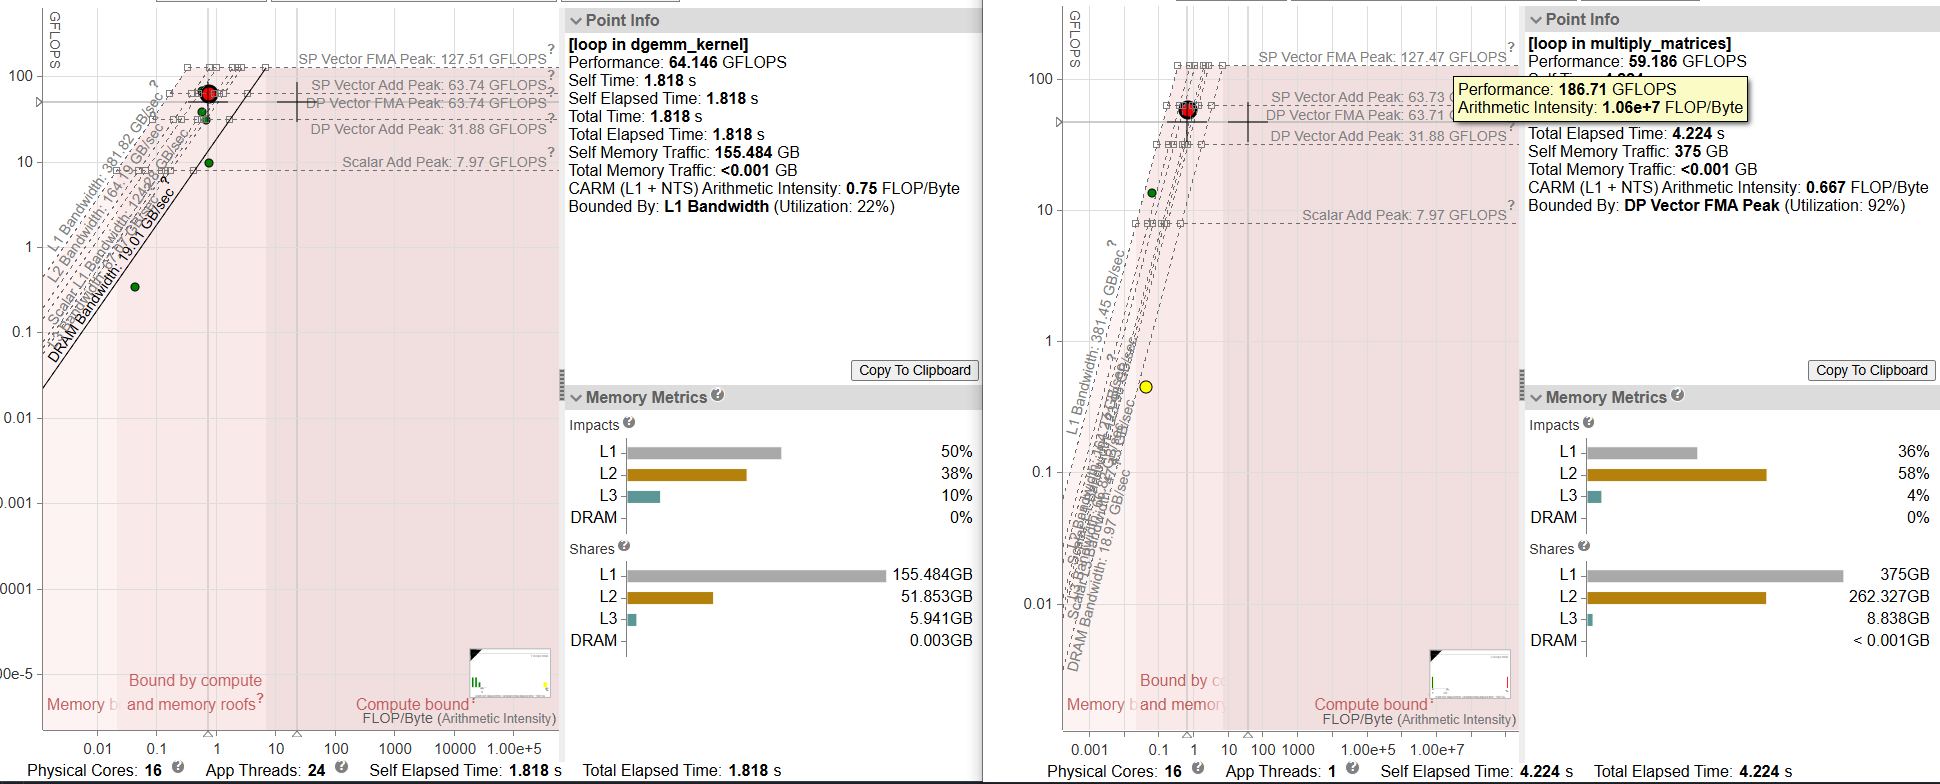
\includegraphics[width=1\textwidth]{Images/openblas_vs_blas_roofline.png}
\caption{Roofline comparison between the original \texttt{OpenBLAS} (left) and our custom implementation (right).}
\label{fig:openblas_vs_blas_roofline}
\end{figure}

As expected, the original \texttt{OpenBLAS} implementation achieves a slightly higher throughput of \textbf{64.146 GFLOPS}. It is classified as bounded by \textbf{L1 Bandwidth}, saturating it with a higher Arithmetic Intensity of $0.75$ FLOP/Byte; there is very little room left for optimization on the machine.

On the other hand, our custom $4 \times 8$ implementation is bounded by the \textbf{DP Vector FMA Peak}, reaching \textbf{59.186 GFLOPS}.As highlighted before, since we use a $4 \times 8$ micro-kernel instead of the $6 \times 8$ one used by OpenBLAS, we do not fully fill all available SIMD registers, hence shifting the primary bottleneck from the memory subsystem (L1 bandwidth) directly to the execution units.

\paragraph{Broader comparison}
The final results are shown in Figure~\ref{fig:blas_vs_openblas}.

\begin{figure}[H]
\centering
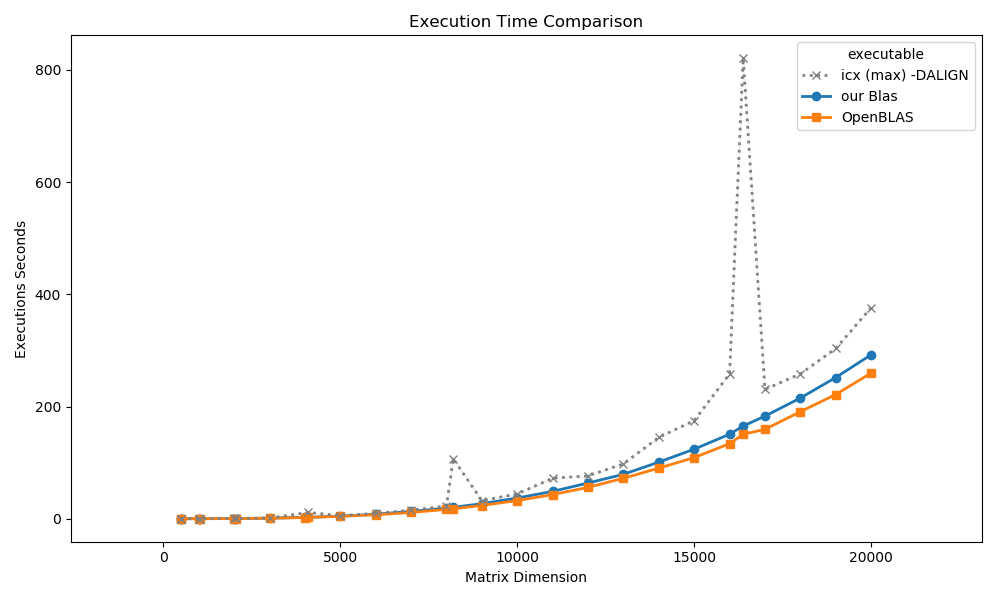
\includegraphics[width=0.8\textwidth]{Images/blas_vs_openblas.png}
\caption{Performance comparison of the original \texttt{OpenBLAS} and our custom implementation 
}
\label{fig:blas_vs_openblas}
\end{figure}

The plot clearly shows a smooth, cubic trends that \emph{finally} matches the suggested complexity of $O(n^3)$, and the already discussed  supremacy of the original version. 

We can now consider completed the quest of the search for the best possible sequential implementation.








% ========================================================================================
% ==================================COMPILER COMPARISON===================================
% ========================================================================================
\subsection{Final Comparison}
As illustrated in Figure~\ref{fig:all_seq_5000}, the in-depth study and progressive refinement of each version yields a consistently faster executable. 

\begin{figure}[H]
\centering
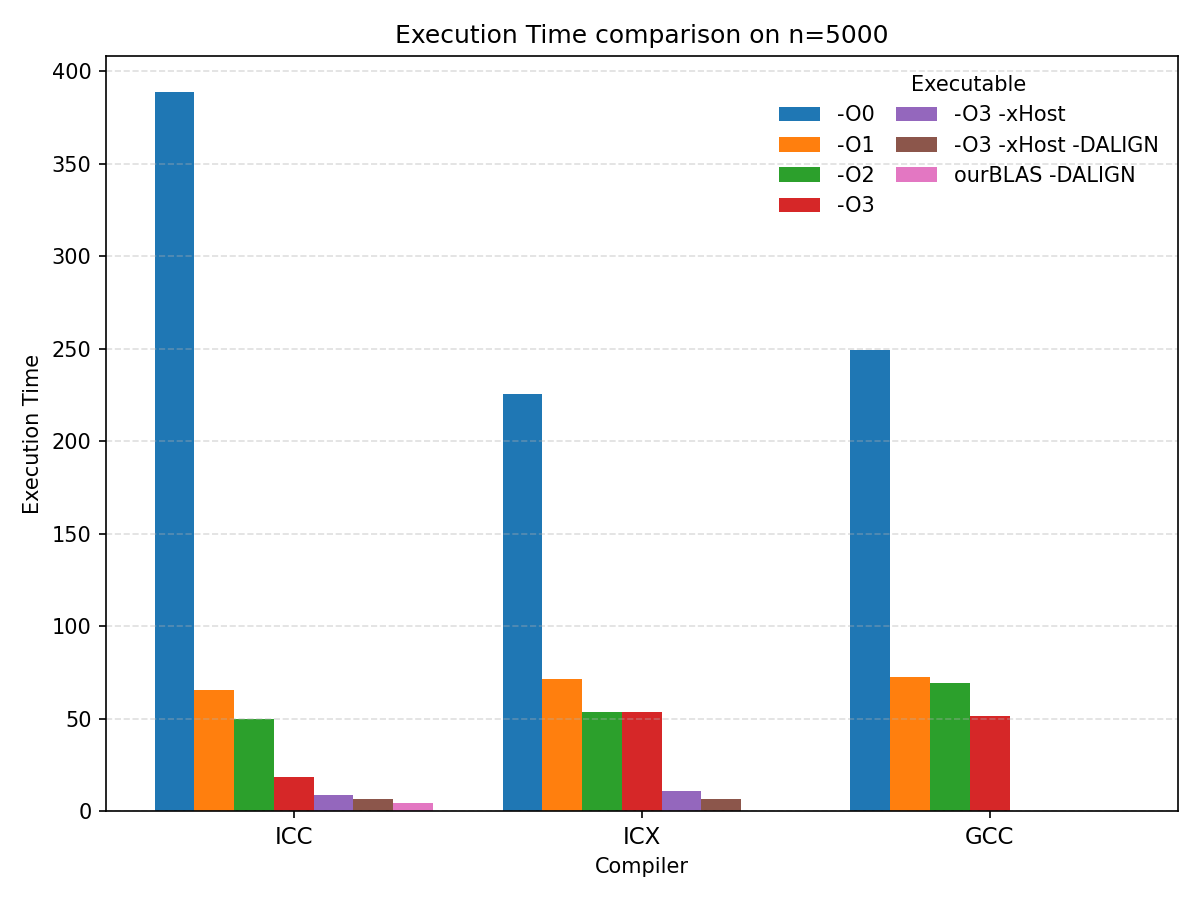
\includegraphics[width=0.8\textwidth]{Images/all_5000.png}
\caption{Comparison of all the previously proposed implementations for $N=5000$.}
\label{fig:all_seq_5000}
\end{figure}

The transition from naive memory accesses to compiler-driven tiling, and finally to explicit SIMD micro-kernels, effectively demonstrates the layers of optimization required to saturate modern hardware.

For the sake of completeness, we ultimately compare our best implementations against the absolute state-of-the-art for Dense Matrix Multiplication on our specific architecture: the \textbf{Intel Math Kernel Library (MKL)}\footnote{Intel MKL (now part of oneAPI) is a highly optimized, proprietary math library developed directly by Intel. It relies on hand-tuned assembly, hardware-specific prefetching, and undocumented architectural features to reach the absolute theoretical peak throughput of Intel processors.}. 

\input{Tables/sequential_comparison}

By treating the Intel MKL performance as our 100\% baseline, we can accurately quantify how each of our iterative versions approaches the hardware's maximum potential across different matrix dimensions. 

Using the GFLOPS computation formula detailed in Section~\ref{subsubsec:metrics}, we demonstrate that our custom implementation successfully achieves approximately \textbf{87\%} of the state-of-the-art peak performance.

\newpage
\section{OpenMP}\label{sec:openmp}

In the preceding sections, we established the maximum practical peak performance achievable through sequential execution on a single core. Proceeding with the iterative optimization strategy proposed in Section~\ref{sec:sequential}, we now exploit the shared-resources paradigm by utilizing OpenMP. 

This approach allows us to further increase the computational throughput by distributing the workload across logical threads mapped to physical cores in the CPU (details in  \ref{tab:cpu_specs}).

We begin by applying basic multi-threading to the original baseline implementation to observe the initial parallel scaling behavior. Subsequently, we explore the parallelization of our custom \textbf{BLAS-like} implementation, examining the impact of thread distribution, hardware binding, and scheduling strategies. 

Lastly, we evaluate our optimized multi-threaded implementations against state-of-the-art libraries (alredy evaluated in single-thread mode) \textbf{multi-threaded OpenBLAS} and the \textbf{Intel Math Kernel Library (MKL)}.

\subsection {Compiler Directives: \texttt{Pragmas}} 
In particular, we leverage OpenMP by explicitly guiding the compiler through standardized \texttt{\#pragma} directives. These hints allow us to dictate thread creation, work distribution, and low-level execution policies without altering the underlying sequential algorithm:

\begin{itemize}
    \item \textbf{\texttt{\#pragma omp parallel}:} Initiates a parallel region, instructing the compiler to fork a team of threads to execute the enclosed block of code concurrently.
    
    \item \textbf{\texttt{\#pragma omp for}:} A work-sharing construct that partitions the iterations of the immediately following loop, distributing the workload among the active thread \emph{team}; we will use it directly merged 
    with the previous directive in a single directive (\texttt{\#pragma omp parallel for}).
    
    \item \textbf{\texttt{schedule(type, chunk\_size)}:} Used to explicitly define how loop iterations are mapped to threads. We will manually tune the schedule type (\texttt{static}, \texttt{dynamic}) and the block size, to find empirically the optimal workload distribution between threads and cores.
\end{itemize}

\paragraph{Hyperparameter tuning}

Maintaining the experimental methodology established in previous sections, the execution environment is parameterized at runtime via command-line arguments $$ \texttt{--threads T} \qquad \texttt{--schedule S} \qquad \texttt{--block-size B} $$

This flexibility allows for a empirical investigation of parallel tuning and scalability. In the following sections, we analyze these results to address three fundamental questions:

\begin{itemize}
\item \textbf{Concurrency}: What is the saturation point where increasing the thread count ceases to improve GFLOPS?
\item \textbf{Scheduling}: Do the scheduling policy (along with the chunk size) impact the performance gain?
\item \textbf{Affinity}: Can we further optimize the performances by explicitly binding threads to physical cores to minimize cache-coherency traffic?
\end{itemize}

\subsection{Original implementation}

The code of the previously proposed implementation is shown in Listing~\ref{lst:naive_mm}.
Since in the section above we benchmark the compiled code on matrices of size multiple of 8 and in any case ensured to be like that due to the \texttt{-DALIGN} flag, for consistency purposes we will also include that flag in every proposed tests. 

Also for continuity purposes we will show results from \textbf{ICC}, omitting the one from ICX and GCC (since they do not provide any observation  that was not already discussed).

The integrated OpenMP implementation for the baseline algorithm is detailed in Listing~\ref{lst:orig_openmp}.

\begin{lstlisting}[style=CStyle, caption={Original algorithm with OpenMP directives: the parametrization is managed at runtime.}, label={lst:orig_openmp}]
int n_threads;
omp_sched_t runtime_schedule_type;
int block_size;

void multiply_matrices(int n,
    m_type (*restrict A)[n], m_type (*restrict B)[n], m_type (*restrict C)[n])
{
    (*@\textcolor{red}{omp\_set\_schedule(runtime\_schedule\_type, block\_size);} @*)
    (*@\textcolor{red}{omp\_set\_num\_threads(n\_threads);} @*)
    
    (*@\textcolor{red}{\#pragma omp parallel for shared(A, B, C, n) schedule(runtime)}   @*)   
    for (int i = 0; i < n; ++i)
        for (int k = 0; k < n; k++)
            for (int j = 0; j < n; ++j)
                C[i][j] += A[i][k] * B[k][j];
}
\end{lstlisting}

\subsubsection{Concurrency}
Now that we have a general overview of the problem, we can start with the empirical investigation.
First, we can propose an \emph{educated guess} about the best number of threads we can concurrently use.

As reported in Table~\ref{tab:cpu_specs}, the studied hardware integrate 8 single-threaded core, and 8 2-way simultaneous-multithreaded cores; we can hence suppose the sweet-spot will in be in the range 16-24 (more than that will produce more threads than cores, wasting computational time by executing context-switches).

The empirical results are shown in Figure~\ref{fig:orig_tune_t}, and they confirm our hypothesis choosing \textbf{\texttt{T=24}} as the best choice.

\begin{figure}[H]
    \centering
    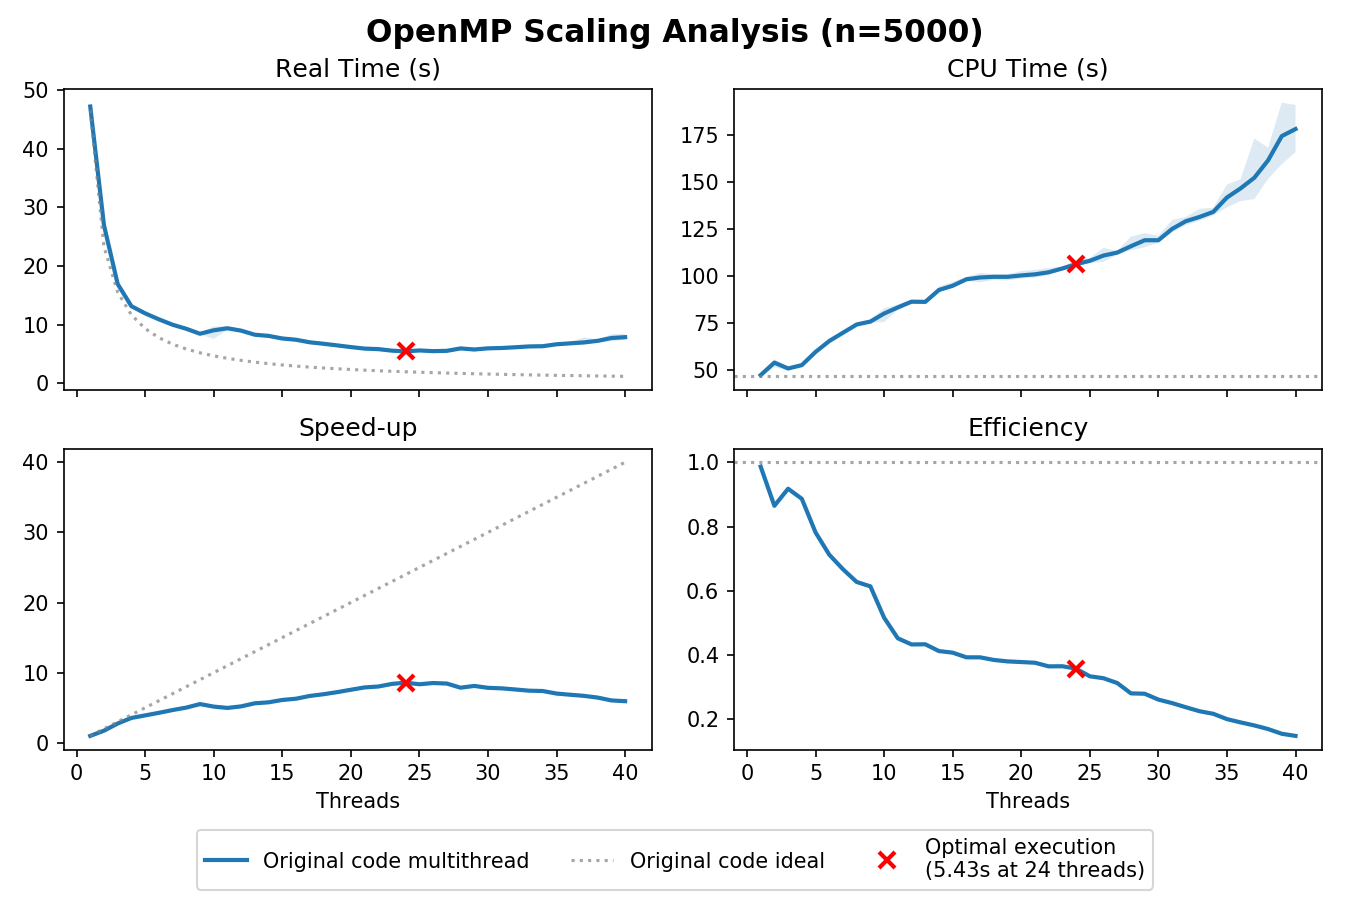
\includegraphics[width=\textwidth]{Images/orig_t_tuning.png}
    \caption{Hyper-parameter tuning of the naive algorithm on $T$, evaluated on matrix \texttt{n=5000} }
    \label{fig:orig_tune_t}
\end{figure}

Comparing these results with the equivalent sequential baseline (which computes a matrix of size \texttt{n=5000} in \textbf{6.5 seconds}), we evaluated the multi-threaded execution using the \emph{Speed-up} and \emph{Efficiency} metrics (introduced in Section~\ref{subsubsec:metrics}). 

The results show a performance degrated so much that it cannot only be caused by multi-threading overhead operations: investigating the compiler's optimization reports clearly shows that introducing the OpenMP directives forces the compiler to avoid the aggressive loop transformations that it typically applies under the \texttt{-O3} flag. 

Once assessed this problem, further hyper-parameter tuning of the naive algorithm is futile. Consequently, we will abandon this implementation and transition to exploring only our custom BLAS-like implementation.





\subsection{BLAS-like implementation}
Given the high complexity of the algorithm (details in Appendix~\ref{subsec:openblas}), it could be modified in several ways (e.g., each thread having its own \texttt{packedA} and \texttt{packedB}, or sharing \texttt{packedB} while keeping \texttt{packedA} private).

Ultimately, the empirically proven best choice is the one proposed in Listing~\ref{lst:blas_like_openmp}: each thread allocates its own \texttt{packedA} and \texttt{packedB} structures and works only on its assigned subset of rows (the \texttt{\#pragma omp for} directive subdivides the workspace of that iteration).

This proved to be the optimal approach because the high capacity of the L3 cache (30 MB) can easily store all the \texttt{packedB} blocks across the threads. Each \texttt{packedB} block is $512 \times 256 \times 8$ bytes (1 MB), meaning the L3 cache can comfortably accommodate up to 30 of them. Additionally, each L2 cache (1.25 MB) can efficiently fit up to two \texttt{packedA} blocks, as each one is $256 \times 256 \times 8$ bytes (0.5 MB).

\begin{lstlisting}[style=CStyle, caption={Blas-like implementation with OpenMP directives}, label={lst:blas_like_openmp}]
extern int n_threads;
extern omp_sched_t runtime_schedule_type;
extern int block_size;

void multiply_matrices( int n, 
    double (*restrict A)[n], 
    double (*restrict B)[n], 
    double (*restrict C)[n]) 
{
    
    (*@\textcolor{red}{omp\_set\_schedule(runtime\_schedule\_type, block\_size);} @*)
    (*@\textcolor{red}{omp\_set\_num\_threads(n\_threads);} @*)    
    
    (*@\textcolor{red}{\#pragma omp parallel shared(A, B, C, n)} @*)   
    {
        const PackedA_t packedA = _mm_malloc(MC * KC * sizeof(double), 64);
        const PackedB_t packedB = _mm_malloc(NC * KC * sizeof(double), 64);

        (*@\textcolor{red}{\#pragma omp for schedule(runtime)} @*)   
        for (int j = 0; j < n; j += NC) {
            int nc = MIN(NC, n - j);
            
            for (int k = 0; k < n; k += KC) {
            
                int kc = MIN(KC, n - k);                
                pack_B(n, B, packedB, k, j, kc, nc);  
                
                for (int i = 0; i < n; i += MC) {
                
                    int mc = MIN(MC, n - i);                    
                    pack_A(n, A, packedA, i, k, mc, kc);
                    
                    for (int ir = 0; ir < mc; ir += MR)
                        for (int jr = 0; jr < nc; jr += NR)
                            kernel_4x8(n, C,
                                    packedA[ir / MR],
                                    packedB[jr / NR],
                                    kc, i + ir, j + jr);
                }
            }
        }

        _mm_free(packedA);
        _mm_free(packedB);
    }
}
\end{lstlisting}

Notably, this approach introduces significant memory bandwidth overhead. Because the \texttt{\#pragma omp for} directive distributes the outer $j$ loop, each thread must independently execute \texttt{pack\_A}, thereby redundantly fetching and packing the exact same blocks of matrix $A$ from main memory $T$ times. Resolving this redundancy is non-trivial; it requires abandoning simple loop-level parallelization in favor of a Single Program, Multiple Data (SPMD) architecture with explicit thread synchronization barriers to safely share packed buffers \footnote{As demonstrated in Section~\ref{subsec:openmp_comparisons}, state-of-the-art (SOTA) libraries substantially outperform this baseline. SOTA implementations, such as OpenBLAS, achieve peak memory bandwidth by dynamically sharing packed buffers across thread teams and utilizing hardware-specific cache-aware optimizations.}. 

Furthermore, we were not capable of acquiring a fully working and readable implementation of those optimizations (to conduct a in-depth analysis). Consequently, this OpenMP integrations is considered sufficient for the purposes of this baseline empirical evaluation.

\subsubsection{Concurrency}
We can now start again with the assessment of the performance of the algorithm as the number of threads changes. Since now the performances are comparable with  the sequential implementation, the matrix size was set to \texttt{n=15000} and every evaluation was repeated for \texttt{3} iterations.

\begin{figure}[H]
    \centering
    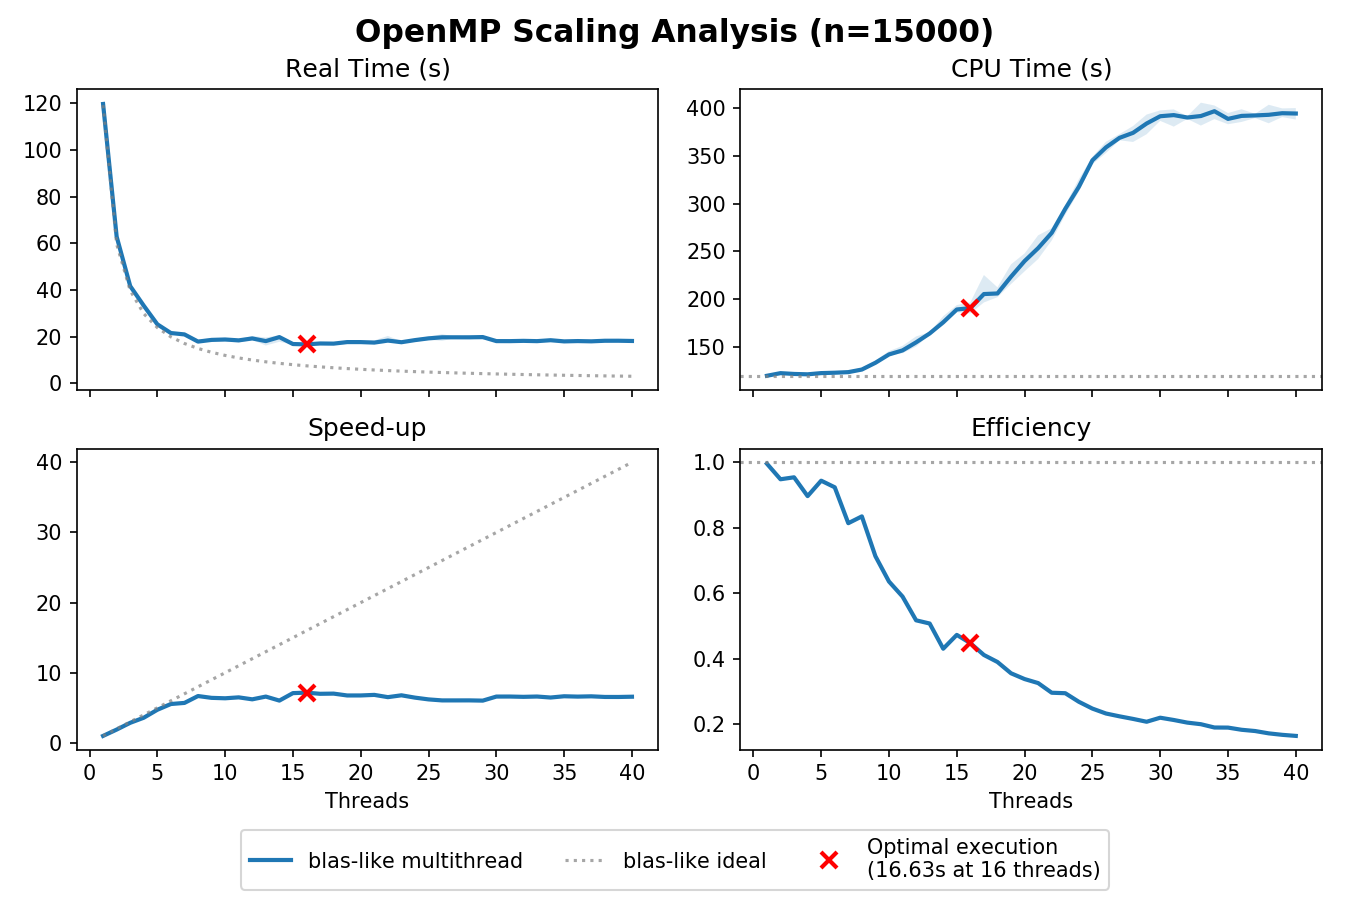
\includegraphics[width=0.85\textwidth]{Images/blas_like_t_tuning.png}
    \caption{Hyper-parameter tuning of the blas-like implementation on $T$, evaluated on matrix \texttt{n=15000} }
    \label{fig:blas_like_tune_t}
\end{figure}

The educated guess is confirmed also in this case, in the Figure~\ref{fig:blas_like_tune_t}; the  performance notably improves with $T \leq 6$ with a quasi-perfect \textbf{speed-up} and \textbf{efficiency}. With more threads, the gain  decreases until the improvements are negligible.

The \textbf{performance degradation} is further motivated by the roofline analysis in Figure~\ref{fig:blas_intel_advisor}: notably, the performance drops from $\approx 59.18 \text{ GFLOPS}$ ($\approx 92\%$ of the \textbf{DP Vector FMA Peak} of $63.71 \text{ GFLOPS}$ --- as shown in the sequential analysis in Figure~\ref{fig:blas_vs_openblas}) to $54\%$ of the roof defined by a multithreaded \textbf{DP Vector FMA Peak} ($744.58 \text{ GFLOPS}$).

\begin{figure}[H]
\centering
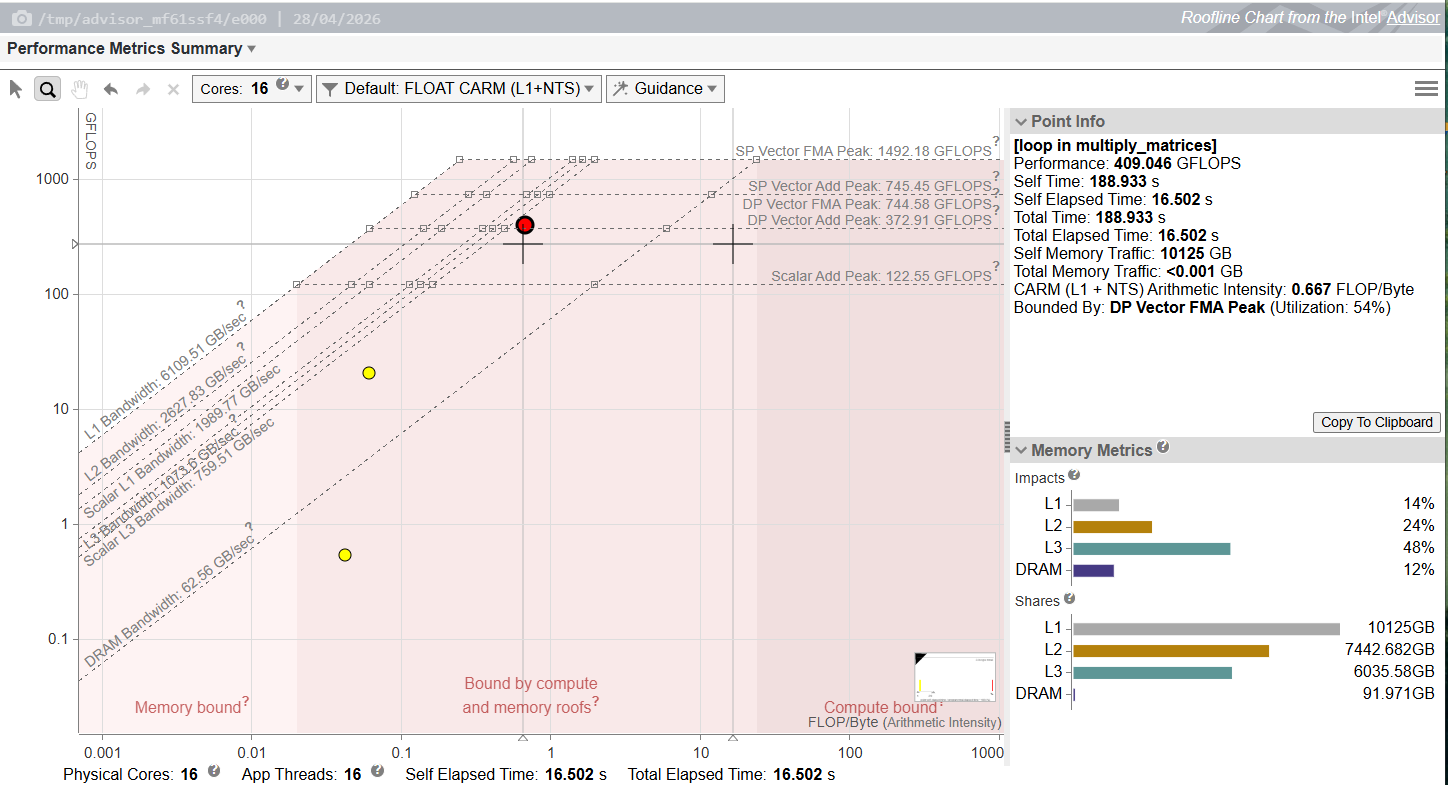
\includegraphics[width=1\textwidth]{Images/blas_intel.png}
\caption{Roofline analysis of our \texttt{Blas-Like} implementatation, executed with \texttt{T=16} on \texttt{n=15000}}
\label{fig:blas_intel_advisor}
\end{figure}

This performance plateau is reflected in the massive data traffic (more than 10,000 GB of L1 traffic, $\approx 48\%$ L3 impact) and low arithmetic intensity. 

\begin{figure}[H]
\centering
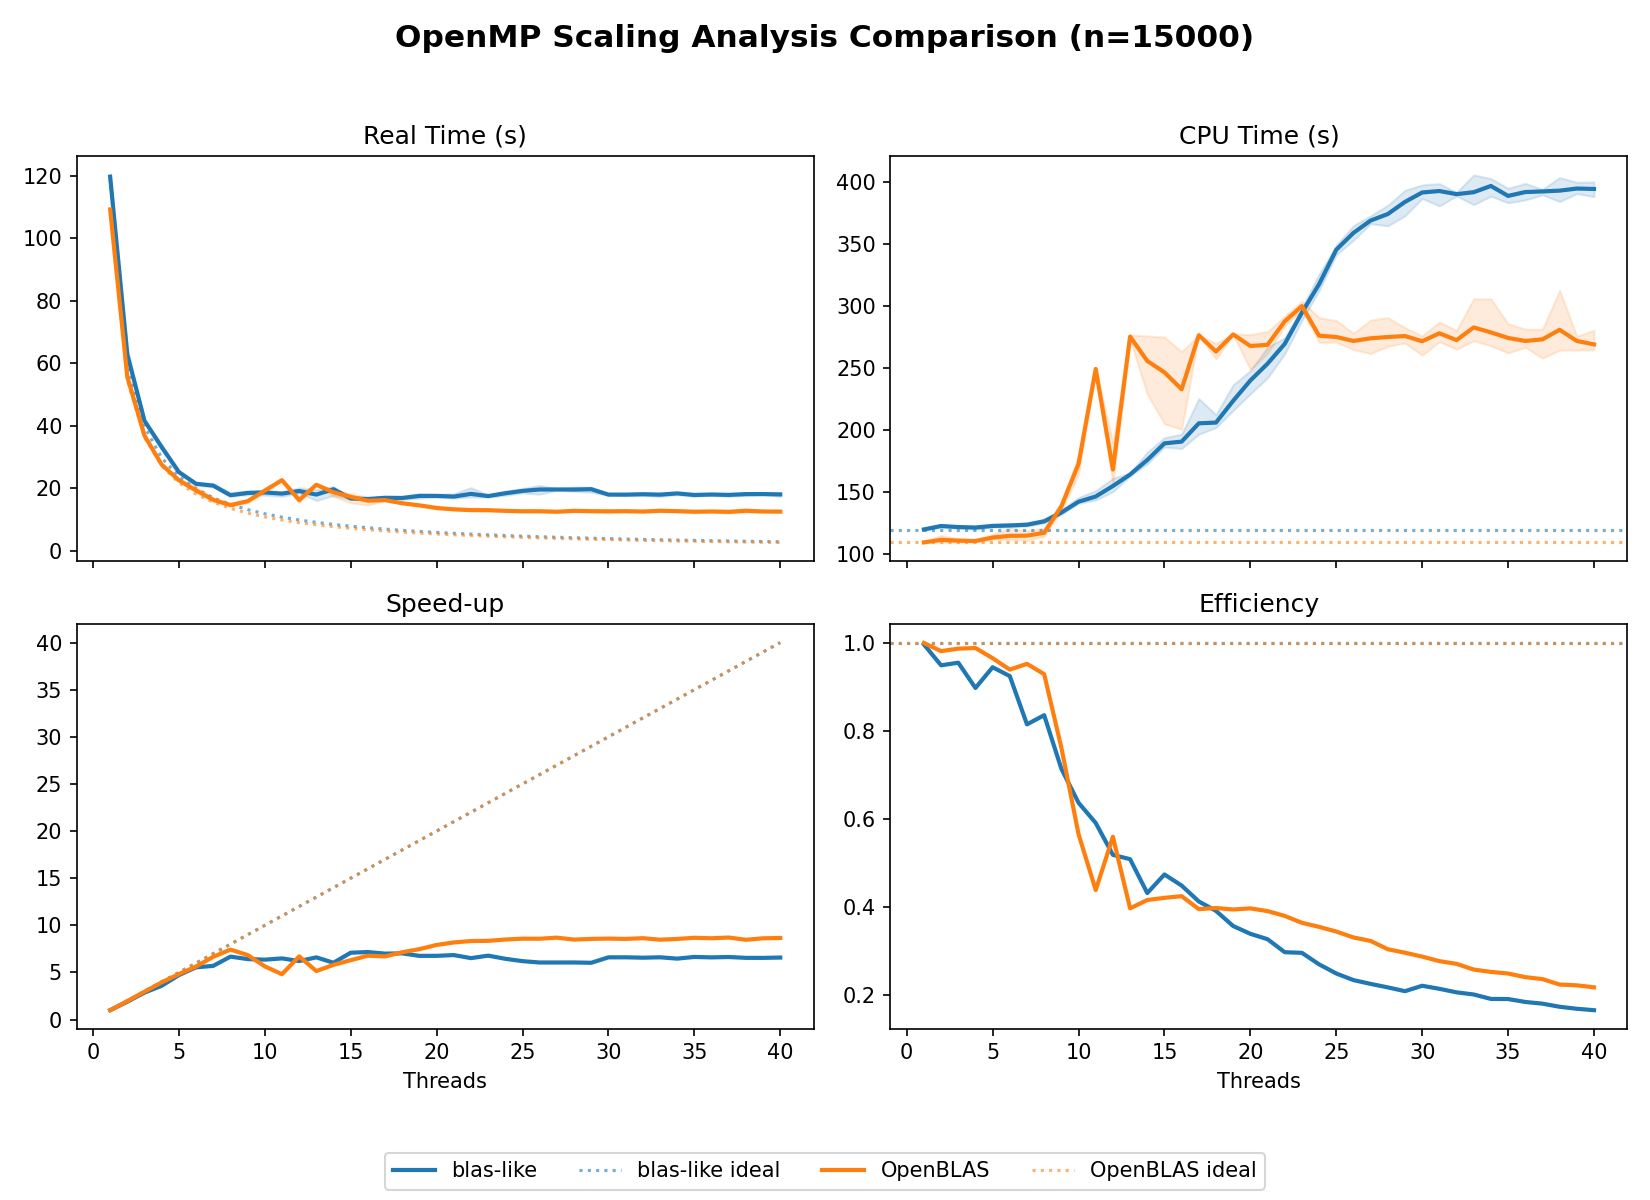
\includegraphics[width=1\textwidth]{Images/blas_comparison_15000.png}
\caption{Performance comparison of the original \texttt{OpenBLAS} and our implementation, in function of \texttt{T} on a matrix \texttt{n=15000}.}
\label{fig:blas_comparison_openmp}
\end{figure}

As Figure~\ref{fig:blas_comparison_openmp} illustrates, even the state-of-the-art OpenBLAS struggles under these constraints; despite a marginally faster absolute execution time, OpenBLAS suffers from severe CPU thrashing beyond 10 threads, yielding a heavily degraded thread efficiency (along with a even more excessive cpu usage).

\vspace{1em}
Having established the inferiority of our implementation, we now attempt to further optimize its multi-thread execution. The pipeline follows a \textbf{greedy approach} to tune the hyperparameters; therefore, for all subsequent tests, the thread count is fixed at \texttt{-{}-threads 16}.

\subsubsection{Scheduling (and Chunk Size)}
To optimize the thread workload, we analyzed the impact of OpenMP scheduling policies (\texttt{static}, \texttt{dynamic}, \texttt{guided}) across varying chunk sizes. Given the matrix size $n=15000$ and a macro-kernel column block $NC=512$, the parallelized outer loop executes  $\lceil 15000 / 512 \rceil = 30$ iterations of the outer (parallelized) loop. 

This coarse granularity, implemented to maximize the usage of the different levels of caches,  dictates the scheduling behavior:
 
\begin{itemize}
    \item \textbf{Thread Starvation (Chunk Size $> 1$):} With only 30 total iterations available to $T=16$ threads, increasing the chunk size immediately causes hardware under-utilization. A chunk size of $2$ yields 15 blocks (leaving 1 thread idle); a chunk size of $8$ leaves 12 threads idle; and any chunk size $\geq 32$ forces purely sequential execution.
    \item \textbf{Load Imbalance:} While the default \texttt{static} policy has minimal overhead, it assumes equal work per iteration. However, the final iteration only computes $15000 \pmod{512} = 152$ columns, finishing significantly faster than the rest. \texttt{static} scheduling forces threads to idle at the implicit barrier while waiting for full-sized chunks to complete.
\end{itemize}

\begin{figure}[H]
    \centering
    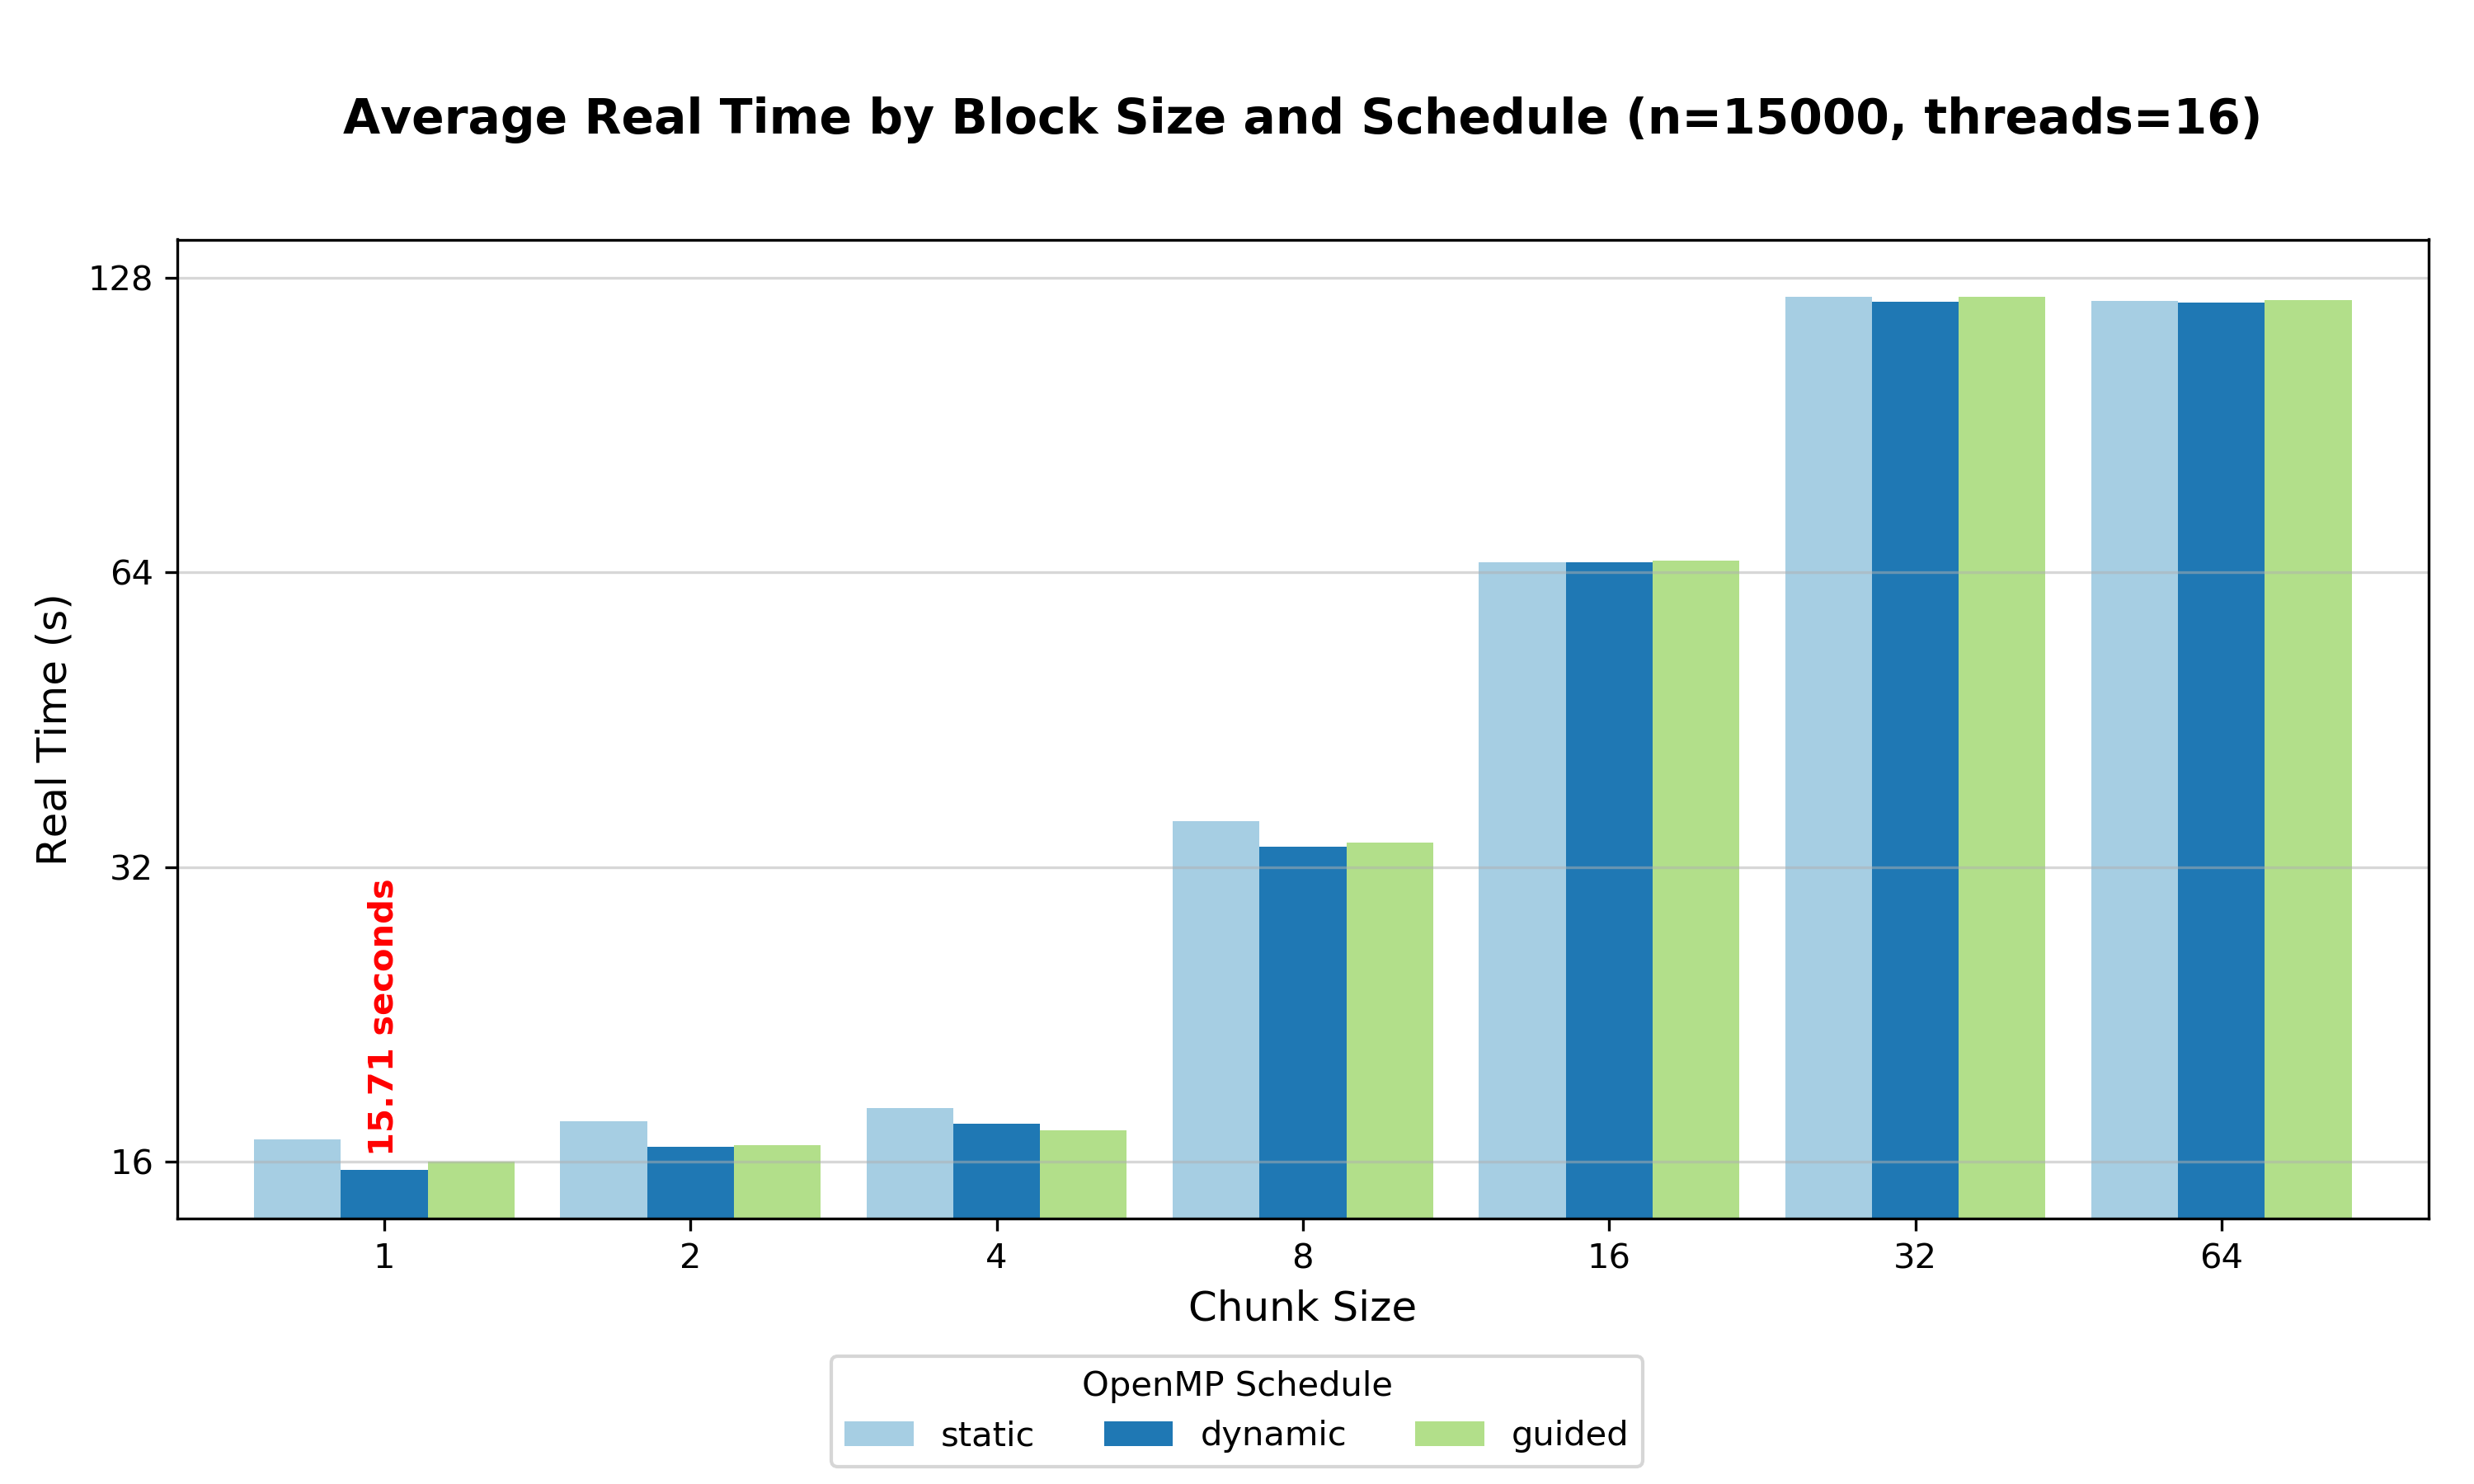
\includegraphics[width=1\textwidth]{Images/blas_like_scheduling.png}
    \caption{Average execution time across varying chunk sizes and scheduling policies, on a matrix n=15000 and T=16.}
    \label{fig:blas_scheduling}
\end{figure}

As demonstrated in Figure~\ref{fig:blas_scheduling}, the margin for improvement is extremely narrow. Configurations with chunk sizes $\geq 8$ result in performance degradation. Consequently, to guarantee full core utilization, the chunk size must be strictly restricted to \texttt{1}. 

Under those observations, the best possible choice is to use the dynamic scheduling by passing   \texttt{-{}-schedule 2 --block-size 1}; this improvement lowers the time down to \textbf{15.71 seconds}.


\subsubsection{Affinity}
Lastly, to (try to) mitigate cache thrashing and maximize hardware utilization, we evaluated the impact of thread affinity. OpenMP controls thread binding through two environment variables:
\begin{itemize}
    \item \texttt{OMP\_PLACES}: Defines the hardware granularity (\texttt{threads}, \texttt{cores}, or \texttt{sockets}) where threads are mapped to be executed.
    \item \texttt{OMP\_PROC\_BIND}: Dictates the distribution policy (\texttt{master}, \texttt{close}, or \texttt{spread}) of threads across the defined places.
\end{itemize}

\begin{figure}[H]
    \centering
    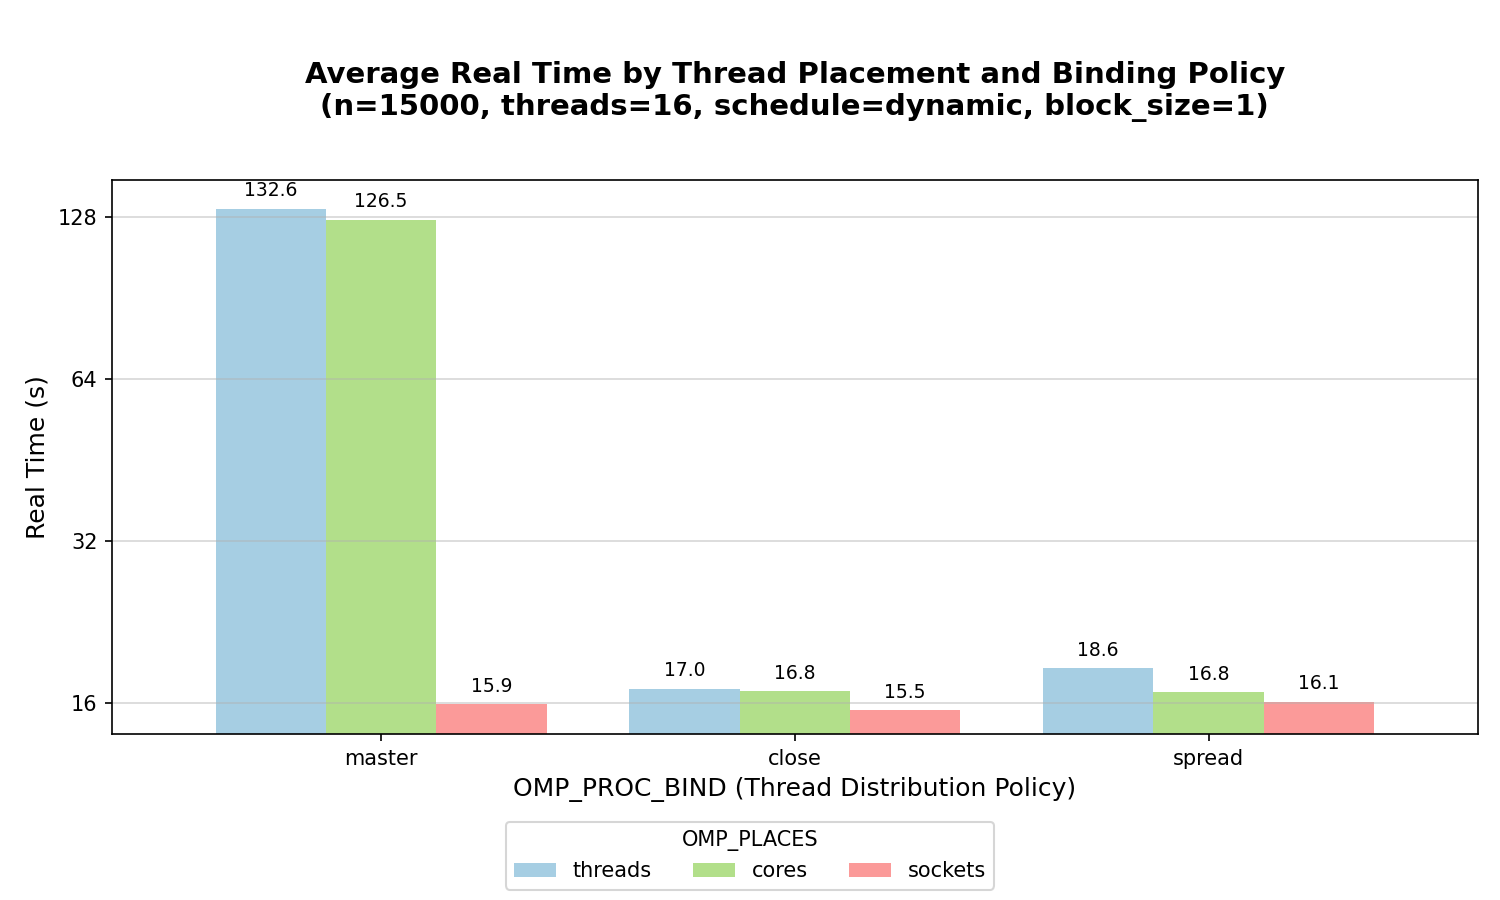
\includegraphics[width=1\textwidth]{Images/blas_like_binding_bind.png}
    \caption{Execution time varying with each possible mapping setting.}
    \label{fig:blas_affinity}
\end{figure}

As illustrated in Figure~\ref{fig:blas_affinity}, the hardware binding configuration can nullify the performance gain of the multithread approach. The \texttt{master} policy catastrophically serializes the workload ($\approx 132\text{s}$) when restricted to a single thread or core, as all 16 threads are forced to multiplex onto a severely limited execution unit. It only recovers when the boundary is expanded to the entire \texttt{socket} (i.e on different cores). 

In contrast, the \texttt{close} and \texttt{spread} policies maintain highly stable performance across all hardware granularities. The absolute optimal configuration is achieved by combining the \texttt{close} policy with \texttt{sockets} ($15.5\text{s}$).



\subsection{Final comparisons}
\label{subsec:openmp_comparisons}

For completeness, we evaluate the performance scaling of the algorithms provided by \texttt{Intel MKL} (Figure~\ref{fig:mkl_tune_t}). Since the library natively manages multithreading, the thread count only needs to be defined dynamically at runtime using its API call \texttt{mkl\_set\_num\_threads(n\_threads)}.

The scaling curves exhibit a clear jagged pattern. This fluctuating behavior is typical of highly optimized libraries like MKL (indeed, it is also present in OpenBLAS, as seen in Figure~\ref{fig:blas_comparison_openmp}). As previously discussed, further speculations regarding these fluctuations is omitted, as they cannot be empirically verified.

\begin{figure}[H]
    \centering
    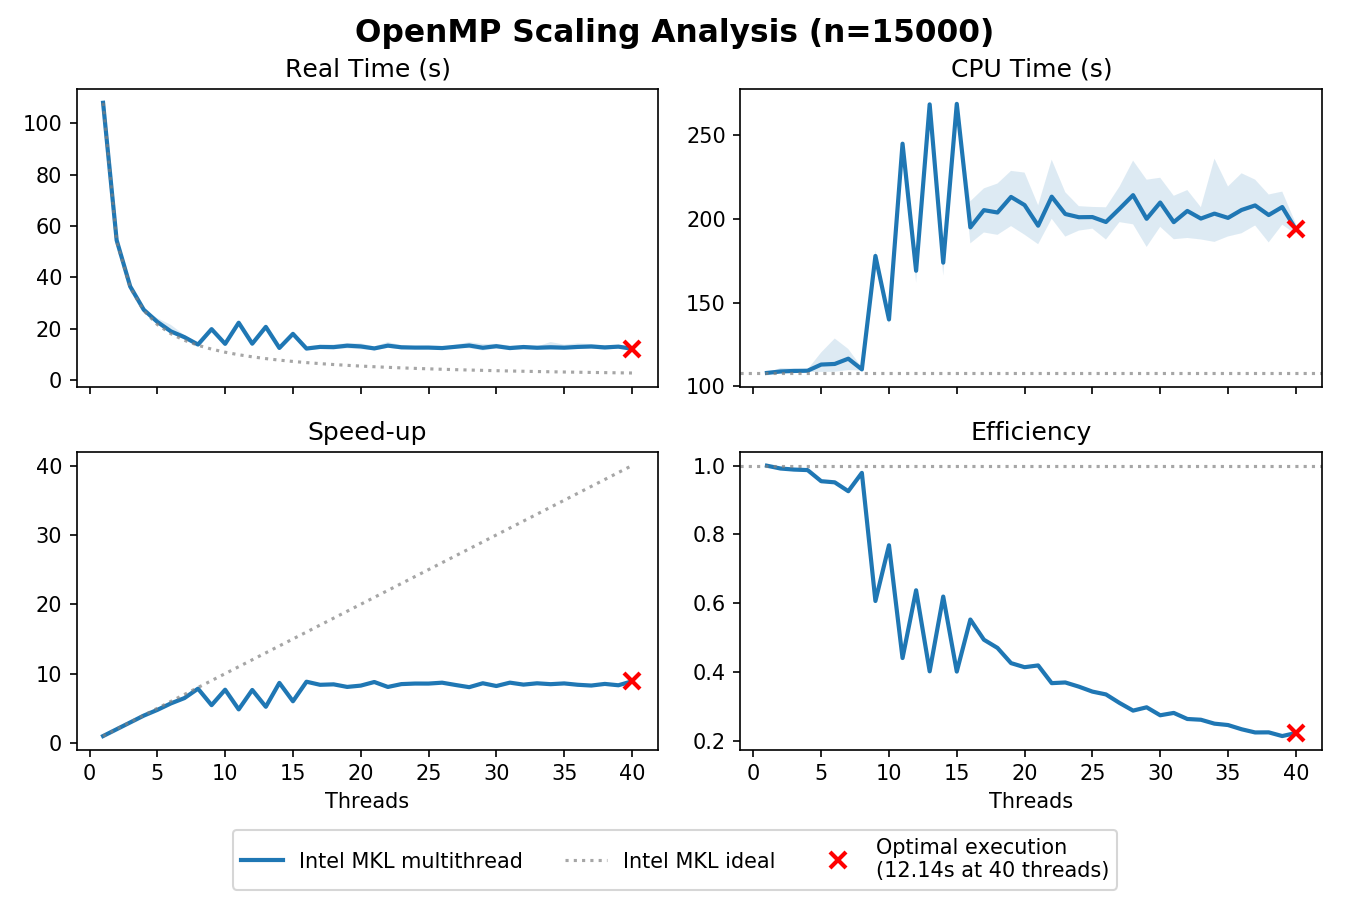
\includegraphics[width=\textwidth]{Images/mkl_t_tuning.png}
    \caption{Hyper-parameter tuning of the Intel MKL implementation on $T$, evaluated on matrix \texttt{n=15000}}
    \label{fig:mkl_tune_t}
\end{figure}


\paragraph{Results Summary}
To summarize the iterative parallel optimization pipeline and contextualize our custom implementations against state-of-the-art libraries, Table~\ref{tab:final_openmp_comparison} aggregates the performance metrics of each major milestone across different matrix sizes.

\begin{table}[H]
\centering
% The resizebox must wrap the ENTIRE threeparttable
\resizebox{\textwidth}{!}{%
  \begin{threeparttable}
    \caption{Performance comparison of the multithreaded implementations across different matrix sizes. Percentages reflect computational throughput (GFLOPS) relative to the Intel MKL baseline. Notably, our version outperform OpenBLAS on bigger matrices.}
    \label{tab:final_openmp_comparison}
    
    \begin{tabular}{l|ccc|ccc|ccc}
    \toprule
     & \multicolumn{3}{c|}{\textbf{N = 5000}} & \multicolumn{3}{c|}{\textbf{N = 10000}} & \multicolumn{3}{c}{\textbf{N = 15000}} \\
    \textbf{Implementation} & \textbf{Time (s)} & \textbf{GFLOPS} & \textbf{\%} & \textbf{Time (s)} & \textbf{GFLOPS} & \textbf{\%} & \textbf{Time (s)} & \textbf{GFLOPS} & \textbf{\%} \\
    \midrule
    Original ($T=24$)                       & 5.360 & 46.65 & 10.01\% & 43.087 & 46.42 & 8.95\% & 149.783 & 45.07 & 8.63\% \\
    Blas-Like ($T=16$, default)             & 0.837 & 298.62 & 64.11\% & 5.789 & 345.47 & 66.62\% & 16.752 & 402.93 & 77.15\% \\
    Blas-Like ($T=16$, dynamic, 1)          & 0.804 & 310.97 & 66.76\% & 4.977 & 401.82 & 77.49\% & 15.571 & 433.49 & 83.00\% \\
    \textbf{Blas-Like (Optimal)}\tnote{1}   & \textbf{0.882} & \textbf{283.32} & \textbf{60.83\%} & \textbf{4.906} & \textbf{407.67} & \textbf{78.61\%} & \textbf{15.571} & \textbf{433.50} & \textbf{83.01\%} \\
    \midrule
    OpenBLAS ($T=16$)                                & 0.662 & 377.37 & 81.02\% & 4.677 & 427.65 & 82.47\% & 16.997 & 397.13 & 76.04\% \\
    \textbf{Intel MKL ($T=16$)}                      & \textbf{0.537} & \textbf{465.77} & \textbf{100.00\%} & \textbf{3.857} & \textbf{518.57} & \textbf{100.00\%} & \textbf{12.925} & \textbf{522.24} & \textbf{100.00\%} \\
    \bottomrule
    \end{tabular}
    
    \begin{tablenotes}
        \footnotesize
        \item[1] Evaluated with tuned affinity settings: \texttt{OMP\_PROC\_BIND=close, OMP\_PLACES=sockets}.
    \end{tablenotes}
  \end{threeparttable}%
}
\end{table}


\newpage
\section{CUDA}\label{sec:CUDA}

\textbf{CUDA} is a parallel computing platform and programming model by NVIDIA that exposes GPUs for general-purpose computing. It provides the core infrastructure to accelerate compute-intensive algorithms, such as matrix multiplication, by distributing the parallel workload across thousands of cores.
The specific CUDA architectural parameters and capabilities utilized in this implementation correspond to the hardware configurations previously detailed in the GPU Hardware Specifications (Section~\ref{sec:GPU spec}). 

\paragraph{CUDA Hierarchy and Execution Model}
The CUDA programming model structures execution through a three-tiered hardware abstraction hierarchy. A kernel invocation from the host instantiates a \textbf{grid} on the device, which is partitioned into independent \textbf{blocks}. Each block encapsulates up to 1024 concurrent \textbf{threads}. Crucially, threads within the same block can synchronize execution and share data via low-latency \textbf{Shared Memory (SMEM)}.

The spatial topology of this hierarchy is defined by the built-in \texttt{dim3} vector types: \texttt{blockDim} determines the thread layout per block, bounded by the architectural limit $$\text{blockDim.x} \times \text{blockDim.y} \times \text{blockDim.z} \leq 1024$$
Consequently, \texttt{gridDim} defines the number of allocated blocks in the grid.

\paragraph{Kernel execution}
In this section we will test different kernels, executed with custom function \emph{launch\_kernel} whose goal is simply to define the grid and the block's size: 

\begin{lstlisting}[style=CStyle, caption={Example code to launch the Naive Kernel: the block's sizes can be defined at runtime. }, label={lst:cuda_launch_kernel}]
extern int cu_block_x, cu_block_y;

void launch_kernel(int n, m_type *dA, m_type *dB, m_type *dC) {
    dim3 block(cu_block_x, cu_block_y);
    dim3 grid(CEIL_DIV(n, cu_block_x), CEIL_DIV(n, cu_block_y));
    kernel<<<grid, block>>>(n, dA, dB, dC);
}
\end{lstlisting}

What happens: 
\begin{itemize}
    \item \texttt{dim3 block(cu\_block\_x, cu\_block\_y)}: defines the dimension of each thread block
    \begin{itemize}
        \item Example: $16 \times 16 = 256$ threads per block
    \end{itemize}
    \item \texttt{dim3 grid(...)}: defines how many blocks are needed to cover the entire matrix
    \item \texttt{kernel<<<grid, block>>>}: CUDA syntax to launch the kernel
    \begin{itemize}
        \item \texttt{grid}: grid configuration
        \item \texttt{block}: block configuration
    \end{itemize}
\end{itemize}
The dimensions of the thread block can be dynamically defined at runtime, allowing for the adjustment of \texttt{cu\_block\_x} and \texttt{cu\_block\_y}.

\paragraph{Experimental methodology}
The CUDA development involved the implementation of various kernel types, starting from the simplest version, defined as \emph{naive}, and then proceeding with increasingly optimized versions, each one fixing the limitations of the previous iteration.

The recorded execution times for the various tests reflect not only the actual matrix multiplication, but also GPU memory allocation for the matrices, data transfers between the host (CPU) and the device (GPU) including the resulting matrix, GPU memory deallocation, and the CUDA kernel launch overhead.
All tests were performed using matrices of size $N = 15000$ to study performance consistently across all implemented kernel types.

\subsection{Kernel 1: Naive Implementation}


For the first kernel, we leverage the \textbf{grid, block, and thread} hierarchy to uniquely assign each thread to a single element of the resulting matrix $C$. This structure allows each thread to compute the dot product of a row from $A$ and a column from $B$ in total autonomy.

\begin{lstlisting}[style=CStyle, caption={Naive CUDA matrix multiplication kernel}, label={lst:cuda_naive_kernel}]
__global__ void kernel(int n, const m_type *A, const m_type *B, m_type *C) {
    int row = blockIdx.y * blockDim.y + threadIdx.y;
    int col = blockIdx.x * blockDim.x + threadIdx.x;
    if (row < n && col < n) {
        m_type sum = 0.0;
        for (int t = 0; t < n; ++t) {
            sum += A[row * n + t] * B[t * n + col];
        }
        C[row * n + col] = sum;
    }
}
\end{lstlisting}

The kernel invocation is handled according to the logic defined in Listing \ref{lst:cuda_launch_kernel}. To optimize performance on a matrix of size \textbf{N=15000}, a runtime hyperparameter optimization phase was performed, focusing on the parameters \textbf{\texttt{cu\_block\_x}
} and \textbf{\texttt{cu\_block\_y}}. This procedure allowed a systematic analysis of the impact of their combinations on execution time. 
The different combinations studied are from powers of two, starting from 2 and going up to 1024.

\begin{figure}[H]
    \centering
    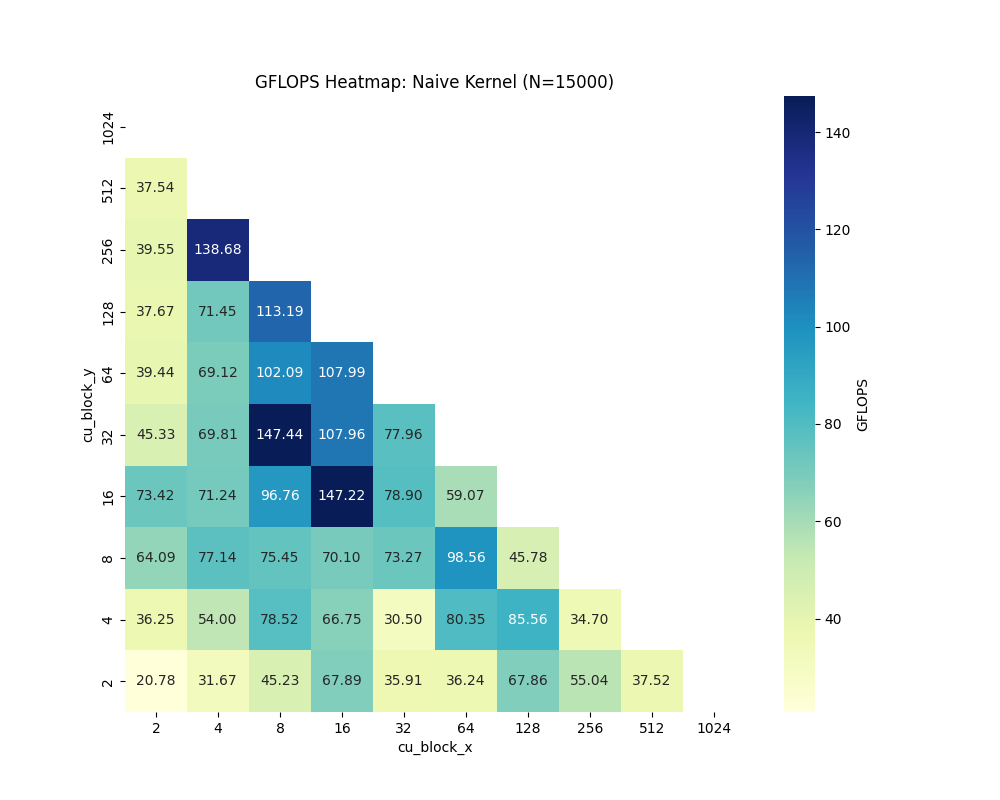
\includegraphics[width=0.8\textwidth]{Images/naive_heatmap.png}
    \caption{HeatMap of hyper-parameter tuning on a matrix $n = 15000$}
    \label{fig:orig_tune_t}
\end{figure} 

\paragraph{Performance Analysis} In the CUDA architecture, instructions are processed in \textbf{warps}, indivisible hardware units of 32 threads operating in SIMT mode. Maximum performance is achieved by saturating the resources of the Streaming Multiprocessors (SMs) and avoiding warp divergence, i.e., idle threads caused by the execution of a heterogeneous set of instructions within the threads of a warp.
\begin{itemize}
    \item \textbf{Optimal Performance:} The best performance (147.4 GFLOPS) is achieved with block sizes of 8x32 and 16x16, both generating 256 threads per block. The two kernels exhibit very similar performance and can therefore be considered equivalent, as the minor discrepancy between the two values is negligible due to measurement noise. This size is optimal because it perfectly aligns with the GPU's hardware limitations, allowing it to activate the maximum possible number of concurrent threads. With a high number of active operations, the hardware effectively masks memory access latencies. 
    
    Additionally, the GPU executes instructions in indivisible groups of 32 threads (warps). Since 256 is a perfect multiple of 32, each warp is completely filled and no computational power is wasted.

\begin{table}[h]
\centering
\begin{tabular}{rrrr}
\toprule
cu\_block\_x & cu\_block\_y & seconds & gflops \\
\midrule
8 & 32 & 45.779 & 147.44 \\
16 & 16 & 45.848 & 147.22 \\
\bottomrule
\end{tabular}
\caption{Best possible performance of the naive kernel (8x32  and 16x16)}
\label{tab:optimal_blocks_perf}
\end{table}

\item \textbf{Worst Performance:} Conversely, the $2 \times 2$ configuration yields the worst performance (20.8 GFLOPS), generating only 4 threads per block. The GPU imposes a physical limit on the number of blocks it can schedule concurrently. 

For example, in the architecture used for this project, the Streaming Multiprocessor (SM) can handle a maximum of 16 blocks simultaneously. If each block contains only 4 threads, the maximum number of active threads per SM will be: $16 \text{ blocks} \times 4 \text{ threads} = 64 \text{ active threads}$. Thus, given a hardware limit of 1024 threads per SM, exactly 6.25\% (64/1024) of the available computing capacity is utilized, leaving the remainder idle. Consequently, this causes a severe waste of resources.

\begin{table}[h]
\centering
\begin{tabular}{rrrr}
\toprule
cu\_block\_x & cu\_block\_y & seconds & gflops \\
\midrule
2 & 2 & 324.519 & 20.80 \\
\bottomrule
\end{tabular}
\caption{Worst possible performance of the naive kernel (2x2)}
\label{tab:worst_perf}
\end{table}

\item \textbf{Hardware Limits (Empty areas):} The cells lacking data represent configurations where the product of $cu\_block\_x \times cu\_block\_y$ exceeds the maximum hardware limit of 1024 threads per block. Such configurations violate architectural constraints, physically preventing the kernel launch.

\end{itemize}

\paragraph{Observation :} Despite both configurations using 256 threads, the $8 \times 32$ block doubles the performance compared to the $32 \times 8$ one ($ 147.4$ GFLOPS vs. $ 73.3$ GFLOPS) due to the different organization of threads within the warp. Since the hardware groups threads by columns, in a $32 \times 8$ block, a warp covers an entire row, forcing the GPU to perform 32 distinct fetches from Global Memory for each iteration. 

In contrast, in the $8 \times 32$ block, the warp folds across 4 rows and 8 columns: threads on different rows reuse the same 8 elements of matrix B already present in memory, drastically reducing latency and doubling efficiency.


\paragraph{Kernel Register Pressure}
To verify the above claims, the flags \texttt{-Xptxas -v} were used to analyze the register pressure specific to the NVIDIA T4 architecture using the naive kernel; the output shows:

\begin{quote}
    \texttt{0 bytes stack frame, 0 bytes spill stores, 0 bytes spill loads \\
    ptxas info : Used 63 registers, used 0 barriers, 384 bytes cmem[0]}
\end{quote}

\begin{itemize}
    \item \textbf{0 bytes spill stores/loads}: Indicates the absence of register spilling. This certifies that the execution does not suffer from bottlenecks due to spilling temporary data into high-latency local memory.
    \item \textbf{Used 63 registers}: Each thread allocates 63 physical registers. On the \textbf{sm\_75} architecture, which features a Register File of \textbf{65,536 registers} per Streaming Multiprocessor (SM), this configuration allows the scheduler to allocate up to 1024 concurrent threads (e.g., 4 blocks of 256). 
    
    Since the total demand ($63 \times 1024 = 64,512$) remains within the physical limit, the hardware successfully saturates the \textbf{theoretical occupancy at 100\%} without inducing register spilling.
    \item \textbf{used 0 barriers}: The kernel does not invoke hardware barrier primitives.
    \item \textbf{Absence of smem data}: The shared memory value is completely absent because the naive approach does not explicitly use it. Each thread performs direct loads from the Global Memory (VRAM). Since there are no arrays declared in the code with the \texttt{\_\_shared\_\_} qualifier, the compiler does not reserve any space in the on-chip shared memory portion.
\end{itemize}

\paragraph{NvProf Analysis} Based on the identified optimal parameters $16 \times 16$ ,equal to the performance 8x32, we will now proceed with a performance profiling analysis using \texttt{nvprof} to examine the kernel behavior in detail taking into account only a few of the most important parameters.

\begin{table}[h]
\centering
\begin{tabular}{lrr}
\toprule
Name & Time (\%) & Time \\
\midrule
\texttt{[CUDA memcpy HtoD]} & 1.61 & 755.88ms \\
\texttt{[CUDA memcpy DtoH]} & 0.80 & 377.45ms \\
\texttt{cudaDeviceSynchronize} & 96.96 & 45.7910s \\
\texttt{cudaMemcpy} & 2.40 & 1.13479s \\
\texttt{cudaMalloc} & 0.61 & 290.09ms \\
\texttt{cudaFree} & 0.01 & 5.9084ms \\
\bottomrule
\end{tabular}
\caption{Nvprof Analysis for Naive Kernel with block 16x16}
\label{tab:nvprof_memory_sync}
\end{table}

\textbf{GPU Activities:}
\begin{itemize}
    \item \texttt{[CUDA memcpy HtoD]} (1.61\% - 755.88ms): Represents the physical transfer of the two operand matrices ($A$ and $B$) from system RAM to GPU VRAM. The execution of two calls justifies a time exactly double that of the inverse operation.
    \item \texttt{[CUDA memcpy DtoH]} (0.80\% - 377.45ms): Transfer of the single result matrix from VRAM to RAM.
\end{itemize}

\textbf{API Calls:}
\begin{itemize}
    \item \texttt{cudaDeviceSynchronize} (96.96\% - 45.79s): It is the explicit barrier point. The time recorded in this API exactly coincides with the kernel execution time: the CPU remains in a blocked state waiting for the device to empty the asynchronous execution queue.
    \item \texttt{cudaMemcpy} (2.40\% - 1.13s): Host-side overhead for orchestrating synchronous transfers.
    \item \texttt{cudaMalloc} (0.61\% - 290.09ms): Computational cost to map and allocate the three matrices in the global address space (VRAM).
    \item \texttt{cudaFree} (0.01\% - 5.9ms): VRAM deallocation operation at the end of the cycle.
\end{itemize}


\paragraph{Limitations and Resume}
Concluding the analysis of this kernel, since \textit{tiling} is missing (which we will see implemented in the next kernel), \textit{Shared Memory} is neither exploited nor used in this kernel. Consequently, the same element of matrix B is read from \textit{Global Memory} multiple times, saturating the memory with redundant data requests. Finally, by computing only a single element of matrix C per thread (each iteration must read and update the same \texttt{sum} accumulator), the GPU fails to overlap multiple mathematical instructions to mask hardware latencies.


\subsection{Kernel 2: Tiling}
A new kernel is introduced that uses the concept of tiling. Tiling is an optimization technique present in CUDA kernels that consists of dividing matrices into smaller blocks (tiles). Each tile is processed separately, often loading the data into shared memory to reduce global memory access costs. 

This allows for better exploitation of data locality and parallelism, improving performance compared to element-by-element processing.
\paragraph{Kernel Call}
The Tiling kernel uses a compile-time constant \texttt{TILE\_WIDTH} to ensure a square geometry. In contrast, the Naive kernel uses run-time parameters because, by not implementing shared memory, it has no allocation constraints and allows dynamic adjustment of the block topology to optimize memory usage. In the Tiling kernel, static shared memory allocation is architecturally necessary so that the compiler can determine the exact memory footprint of each thread block \textit{a priori}.
\begin{lstlisting}[style=CStyle, caption={Code to launch Kernel 2}, label={lst:cuda_coalesced_kernel}]
void launch_kernel(int n, m_type *dA, m_type *dB, m_type *dC) {
    dim3 block(TILE_WIDTH, TILE_WIDTH);
    dim3 grid((n + TILE_WIDTH - 1)/TILE_WIDTH, (n + TILE_WIDTH - 1)/TILE_WIDTH);
    kernel<<<grid, block>>>(n, dA, dB, dC);
}
\end{lstlisting}
\paragraph{Kernel Code}The code performs matrix multiplication on the GPU exploiting the tiling technique, where each thread block works on a portion, called a tile, of the matrix. The data of matrices $A$ and $B$ are loaded into the shared memory of the block, allowing faster access compared to global memory.

Each thread computes an element of the resulting matrix $C$, accumulating the product of the corresponding elements within the tile. Synchronization among the threads occurs via \texttt{\_\_syncthreads()} to ensure that all data are correctly loaded and used. At the end of the computation, the result is written to matrix $C$ only if the thread is within the limits of the matrix. 

\begin{lstlisting}[style=CStyle, caption={CUDA implementation of Kernel 2}, label={lst:Kernel_2_code}]
__global__ void kernel(int n, const m_type *A, const m_type *B, m_type *C) {
    int bx = blockIdx.x, by = blockIdx.y;
    int tx = threadIdx.x, ty = threadIdx.y;

    int row = by * TILE_WIDTH + ty;
    int col = bx * TILE_WIDTH + tx;

    __shared__ m_type sA[TILE_WIDTH][TILE_WIDTH];
    __shared__ m_type sB[TILE_WIDTH][TILE_WIDTH];

    m_type sum = 0.0;
    int numTiles = (n + TILE_WIDTH - 1) / TILE_WIDTH;

    for (int m = 0; m < numTiles; ++m) {
        if (row < n && m * TILE_WIDTH + tx < n)
            sA[ty][tx] = A[row * n + m * TILE_WIDTH + tx];
        else
            sA[ty][tx] = 0.0;

        if (m * TILE_WIDTH + ty < n && col < n)
            sB[ty][tx] = B[(m * TILE_WIDTH + ty) * n + col];
        else
            sB[ty][tx] = 0.0;

        __syncthreads();

        for (int k = 0; k < TILE_WIDTH; ++k) {
            sum += sA[ty][k] * sB[k][tx];
        }

        __syncthreads();
    }

    if (row < n && col < n) {
        C[row * n + col] = sum;
    }
}
\end{lstlisting}

\paragraph{Performance Analysis} Before beginning the analysis of the results, it is important to note that the maximum \texttt{TILE\_WIDTH} value depends on the shared memory available per block and the number of threads. On NVIDIA T4 GPUs, each block can use up to 64 KB of shared memory, but typically only 48 KB is allocated by default for static allocations. This means that \texttt{TILE\_WIDTH} must be chosen so that the memory required by the blocks falls within this limit, taking into account both the number of threads and the data type used. Furthermore, performance was studied by performing multiple iterations for each test to analyze whether there were any discrepancies between the results. Five different iterations were performed for each experiment conducted.

\begin{itemize}
    \item \textbf{\texttt{First Experiment ( 32 x 32 ):}} Kernel 2 clearly surpasses the performance of Kernel 1, exceeding 200~GFLOPS. By exploiting Data Reuse in Shared Memory, fetches from Global Memory are drastically reduced, freeing bandwidth on the bus and masking access latency. 

    \begin{table}[H]
    \centering
    \begin{tabular}{ccc}
    \toprule
    \texttt{TILE\_WIDTH} & Time (s) & GFLOPS \\
    \midrule
    32 & 31.509 & 214.22 \\
    32 & 32.027 & 210.76 \\
    32 & 32.498 & 207.70 \\
    32 & 32.782 & 205.91 \\
    32 & 33.022 & 204.41 \\
    \bottomrule
    \end{tabular}
    \caption{Kernel Performance using 32 x 32}
    \label{tab:kernel2_15000}
    \end{table}
    
    Furthermore, the footprint of a $32 \times 32$ block in double precision requires only 16~KB of Shared Memory (the calculation is: $2 \times (32 \times 32) \times 8 \text{ bytes} = 16,384 \text{ bytes} = 16 \text{ KB}$): falling well within the 48~KB limit of T4 GPUs, it allows the scheduler to allocate more blocks for each Streaming Multiprocessor. 
    
    From the results, however, a variance in execution times can be noted: although the root cause is not clear, a progressive performance decay is evident in the iterations following the first one.
    

    \item \textbf{\texttt{Second Experiment ( 16 x 16 ):}} In the second case where a 16x16 dimension was used, we can notice a drop in GFLOPS, from 214.22 to 197.14. 

    \begin{table}[H]
    \centering
    \begin{tabular}{ccc}
    \toprule
    \texttt{TILE\_WIDTH} & Time (s) & GFLOPS \\
    \midrule
    16 & 34.239 & 197.14 \\
    16 & 35.232 & 191.59 \\
    16 & 36.069 & 187.14 \\
    16 & 36.769 & 183.58 \\
    16 & 37.186 & 181.52 \\
    \bottomrule
    \end{tabular}
    \caption{Kernel Performance using 16 x 16}
    \label{tab:kernel_16x16}
    \end{table}
    
    This is attributable to the lower data reuse. In the Tiling technique, each element loaded from the slower Global Memory to the faster Shared Memory is reused for calculations a number of times equal to the dimension of the tile itself (\texttt{TILE\_WIDTH}). 
    
    With a $32 \times 32$ tile, each fetch in Global Memory is reused 32 times, while with a $16 \times 16$ tile, the same fetch is reused only 16 times. As previously stated for the $32 \times 32$ kernel, a performance degradation can be observed between iterations.


    \item \textbf{\texttt{Third Experiment:}}Following the analysis of the different tile dimensions and the progressive performance degradation observed between iterations, a further test was conducted on the $16 \times 16$ kernel, recording a drastic drop in GFLOPS compared to the previous measurement. 

    \begin{table}[H]
    \centering
    \begin{tabular}{ccc}
    \toprule
    \texttt{TILE\_WIDTH} & Time (s) & GFLOPS \\
    \midrule
    16 & 36.969 & 182.58 \\
    16 & 39.715 & 169.96 \\
    16 & 40.752 & 165.64 \\
    16 & 40.367 & 167.21 \\
    16 & 40.493 & 166.69 \\
    \bottomrule
    \end{tabular}
    \caption{Kernel Performance using 16 x 16 (Repeated)}
    \label{tab:kernel_16x16_final}
    \end{table}
    
\end{itemize}

\paragraph{Note: Cloud Execution Variance} 
As a general comment on the testing methodology, it is crucial to address the high variance and progressive performance degradation observed across iterations in all experiments. Because the Google Colab execution environment operates strictly as a black box, it is impossible to predict, thoroughly understand, or systematically test the root causes of these fluctuations.

Despite keeping the kernel code and execution parameters strictly unchanged, execution times vary significantly between independent tests (some tests had variability of more than $10\%$). This erratic behavior is entirely subdued by Colab's opaque hardware scheduler and its dynamic allocation of shared cloud resources, placing the exact cause of the degradation entirely beyond the scope of user control or local analysis.

    
\paragraph{Kernel Register Pressure}Can see that compared to previous kernels we can notice a different output

\begin{quote}
\texttt{0 bytes stack frame, 0 bytes spill stores, 0 bytes spill loads \\
ptxas info    : Used 42 registers, used 1 barriers, 16384 bytes smem, 384 bytes cmem[0]}
\end{quote}
\begin{itemize}
    \item \textbf{Register Pressure (42 vs 63 registers):} Register usage decreases compared to Kernel 1. The introduction of Shared Memory simplifies the arithmetic for calculating vector indices and reduces the temporary variables active at runtime, significantly lowering the pressure on the Register File.
    \item \textbf{Shared Memory (16384 bytes smem):} The memory footprint confirms the geometric configuration \texttt{TILE\_WIDTH = 32}. The exact calculation is $2 \times (32 \times 32 \times 8 \text{ bytes}) = 16384 \text{ bytes}$ of static shared memory for the two tiles. 
    
    In previous kernels, this parameter was null due to direct access to Global Memory.

    
    \item \textbf{Synchronization (1 barrier):} The PTX compiler reports the allocation of a single hardware barrier at the block level (corresponding to \texttt{\_\_syncthreads()}). This forces the stall of the warps, ensuring that all threads have completed fetching data into Shared Memory before starting arithmetic operations.
\end{itemize}
\vspace{20px}

\paragraph{Nvprof Analysis} Here are the results of using Kernel 32x32 :
\begin{table}[h]
\centering
\begin{tabular}{lrr}
\toprule
Name & Time (\%) & Time \\
\midrule
\texttt{[CUDA memcpy HtoD]} & 2.59 & 780.14ms \\
\texttt{[CUDA memcpy DtoH]} & 1.28 & 386.85ms \\
\texttt{cudaDeviceSynchronize} & 95.46 & 29.0082s \\
\texttt{cudaMemcpy} & 3.85 & 1.16866s \\
\texttt{cudaMalloc} & 0.65 & 197.03ms \\
\texttt{cudaFree} & 0.02 & 6.0008ms \\
\bottomrule
\end{tabular}
\caption{Nvprof Analysis of Kernel 2}
\label{tab:nvprof_analysis_updated}
\end{table}

\begin{itemize}
    \item \texttt{cudaDeviceSynchronize}: In the naive kernel, the kernel completion wait time stabilized at 45.79 seconds. In Kernel Tiling, however, the value dropped to 29.00 seconds. This demonstrates the effectiveness of shared memory.
    \item \texttt{[CUDA memcpy HtoD]} and \texttt{[CUDA memcpy DtoH]}: The absolute times for data transfers from device to host and vice versa remain almost constant between the two versions. The tiling optimization acts solely on the access pattern to the GPU internal memory, not altering the volume of data exchanged between Host and Device.
    \item \texttt{cudaMemcpy}: The slight increase is a direct consequence of the physical time increment of HtoD/DtoH.
    \item The remaining values remained practically unchanged.
\end{itemize}

\subsection{Final Comparison} 

As a final baseline test, the \textbf{cuBLAS} library was employed to establish peak achievable performance. As observed, with the exception of very small workloads, this implementation performs significantly better than all previous custom kernels.

\begin{table}[H]
\centering
\resizebox{\textwidth}{!}{%
  \begin{threeparttable}
    \caption{CUDA Kernel's performance comparison. Percentages reflect computational throughput (GFLOPS) relative to the cuBLAS baseline.}
    \label{tab:final_cublas_comparison_selected}
    \begin{tabular}{l|ccc|ccc|ccc|ccc}
    \toprule
     & \multicolumn{3}{c|}{\textbf{N = 1000}} & \multicolumn{3}{c|}{\textbf{N = 5000}} & \multicolumn{3}{c|}{\textbf{N = 10000}} & \multicolumn{3}{c}{\textbf{N = 15000}} \\
    \textbf{Implementation} & \textbf{Time (s)} & \textbf{GFLOPS} & \textbf{\%} & \textbf{Time (s)} & \textbf{GFLOPS} & \textbf{\%} & \textbf{Time (s)} & \textbf{GFLOPS} & \textbf{\%} & \textbf{Time (s)} & \textbf{GFLOPS} & \textbf{\%} \\
    \midrule
    Kernel 1 (16x16) & 0.330 & 6.06 & 121.82\% & 1.600 & 156.25 & 82.88\% & 11.034 & 181.26 & 80.85\% & 42.411 & 159.16 & 69.10\% \\
    Kernel 2 (32x32) & 0.307 & 6.51 & 130.94\% & 1.411 & 177.18 & 93.98\% & 9.973  & 200.54 & 89.45\% & 33.582 & 201.00 & 87.26\% \\
    \midrule
    \textbf{cuBLAS}  & \textbf{0.402} & \textbf{4.98} & \textbf{100.00\%} & \textbf{1.326} & \textbf{188.54} & \textbf{100.00\%} & \textbf{8.921} & \textbf{224.19} & \textbf{100.00\%} & \textbf{29.304} & \textbf{230.34} & \textbf{100.00\%} \\
    \bottomrule
    \end{tabular}
  \end{threeparttable}%
}
\end{table}

Analyzing the table, it is evident that for very small values of $N$ (such as $N = 1000$), overall performance is poor; notably, the \textbf{cuBLAS} implementation underperforms compared to Kernel 2 despite its theoretical superiority. 
This stems from GPU inefficiency under heavily reduced workloads, where setup latency significantly exceeds effective computation time. Kernel launch and data management introduce fixed overheads that, for small matrices, account for nearly the entire execution duration. 

Rather than a strict application of Amdahl's Law, this bottleneck is primarily dictated by extremely low GPU occupancy. Insufficient thread block generation fails to saturate the available Streaming Multiprocessors (SMs), meaning the hardware cannot effectively use warp scheduling to hide memory access and launch latencies, making the operation a victim of system overhead.

Concluding the analysis, an asymptotic flattening of the throughput curve is observed for Kernel 2 (tiling) and cuBLAS as workloads scale up. Kernel 1, however, scales reasonably well only up to $N = 10000$ (reaching 181.25~GFLOPS), after which it suffers a severe efficiency collapse. At $N = 15000$ and beyond, Kernel 1 regresses from over 80\% down to roughly 69\% of the cuBLAS baseline. Since the naive algorithm lacks \textit{data reuse} optimization, each thread is forced to repeatedly fetch operands directly from Global Memory. 

As the matrix size grows, this dynamic rapidly saturates the memory bus bandwidth, inducing severe memory stalls in the Streaming Multiprocessors. Because all warps are eventually forced to wait on memory transactions, the SM scheduler is unable to swap active warps to hide the latency. Unlike Kernel 1, Kernel 2 demonstrates significantly superior architectural stability by leveraging Shared Memory to bypass the memory wall, ensuring excellent overall performance, albeit confined just below the maximum limit achieved by the highly optimized cuBLAS routines.




\newpage
\section{MPI}\label{sec:mpi}

\subsection{Implementation Strategy}
The Message Passing Interface (MPI) paradigm was used to explore distributed-memory parallelization. Unlike OpenMP, which relies on a shared memory space, MPI requires explicit communication of data between discrete processes. In our approach, the workload was distributed by splitting the first matrix, $A$, by rows among the available processes using \texttt{MPI\_Scatterv}. Since each process needs the full second matrix $B$ to compute its respective rows of the resulting matrix $C$, $B$ was fully broadcasted to all nodes via \texttt{MPI\_Bcast}. Finally, the local results were collected back to the master process using \texttt{MPI\_Gatherv}. 

\begin{lstlisting}[style=CStyle, caption={Optimized kernel i-k-j executed by each MPI process.}, label={lst:mpi_kernel}]
for (int i = 0; i < my_rows; i++) {
    for (int k = 0; k < N; k++) {
        double temp = local_A[i][k];
        for (int j = 0; j < N; j++) {
            local_C[i][j] += temp * B[k][j];
        }
    }
}
\end{lstlisting}

While MPI is natively designed for physical distributed clusters, executing it on a single shared-memory machine highlights the overheads inherently introduced by message passing. By default, MPI implementations do not implicitly share memory among processes on the same host. This drastically increases the RAM footprint (as each process allocates its own full copy of matrix $B$) and introduces substantial data duplication and context-switching penalties that simulate network traffic over the memory bus.

\subsection{Performance and Scalability Analysis}
The algorithm was benchmarked across various matrix sizes ranging from $N = 1024$ up to massive workloads of $N = 15000$, using a number of processes ranging from 1 to 32. 

\begin{figure}[H]
    \centering
    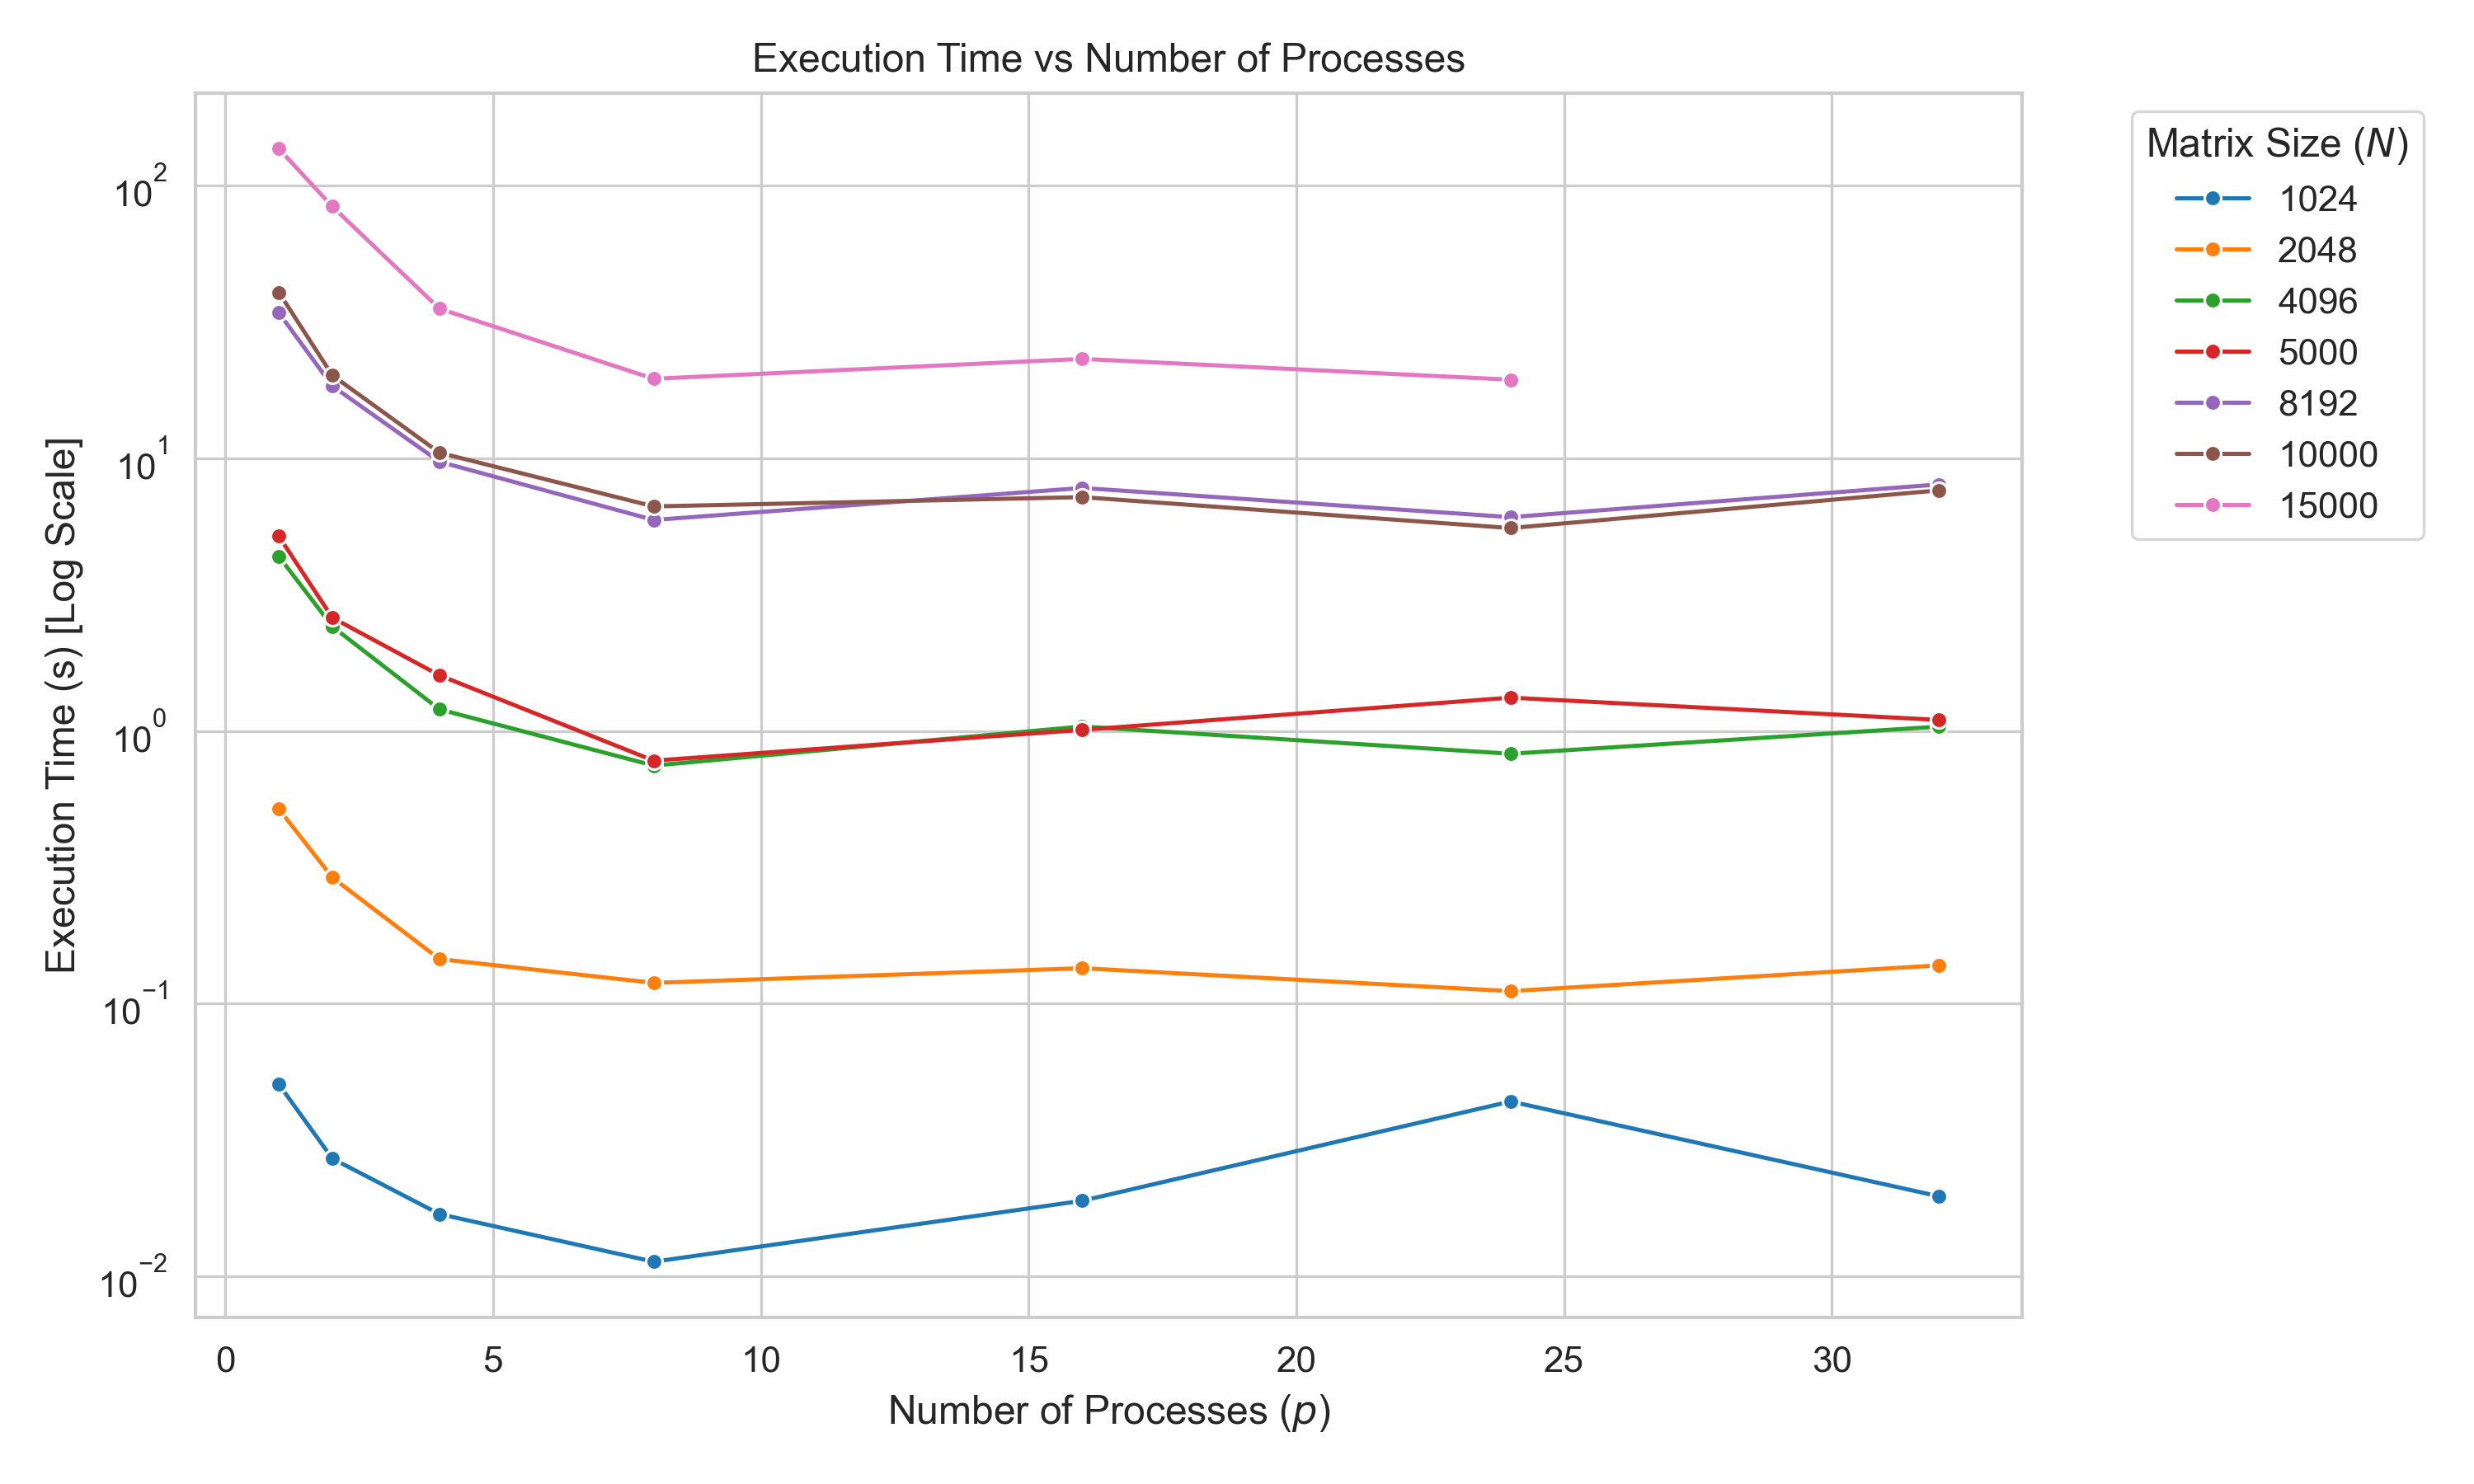
\includegraphics[width=0.8\textwidth]{Images/mpi-plot_1_execution_time.png}
    \caption{Execution time compared to number of processes.}
    \label{fig:mpi_execution_time}
\end{figure} 

The execution time results, shown in Figure~\ref{fig:mpi_execution_time}, demonstrate a consistent performance improvement as the number of processes increases, up to a specific hardware-bound threshold. For $N = 8192$, the sequential baseline execution time was 34.24 seconds, which dropped dramatically to 5.95 seconds at $p=8$. 

Extending the tests to critical dimensions ($N = 10000$ and $N = 15000$) reveals an interesting asymptotic behavior. While for smaller matrices the communication overhead dominates as early as $p=8$, for massive workloads the system benefits from a higher core count, reaching peak performance at $p=24$ for $N=10000$ (5.56s) and $N=15000$ (19.46s).

\begin{figure}[H]
    \centering
    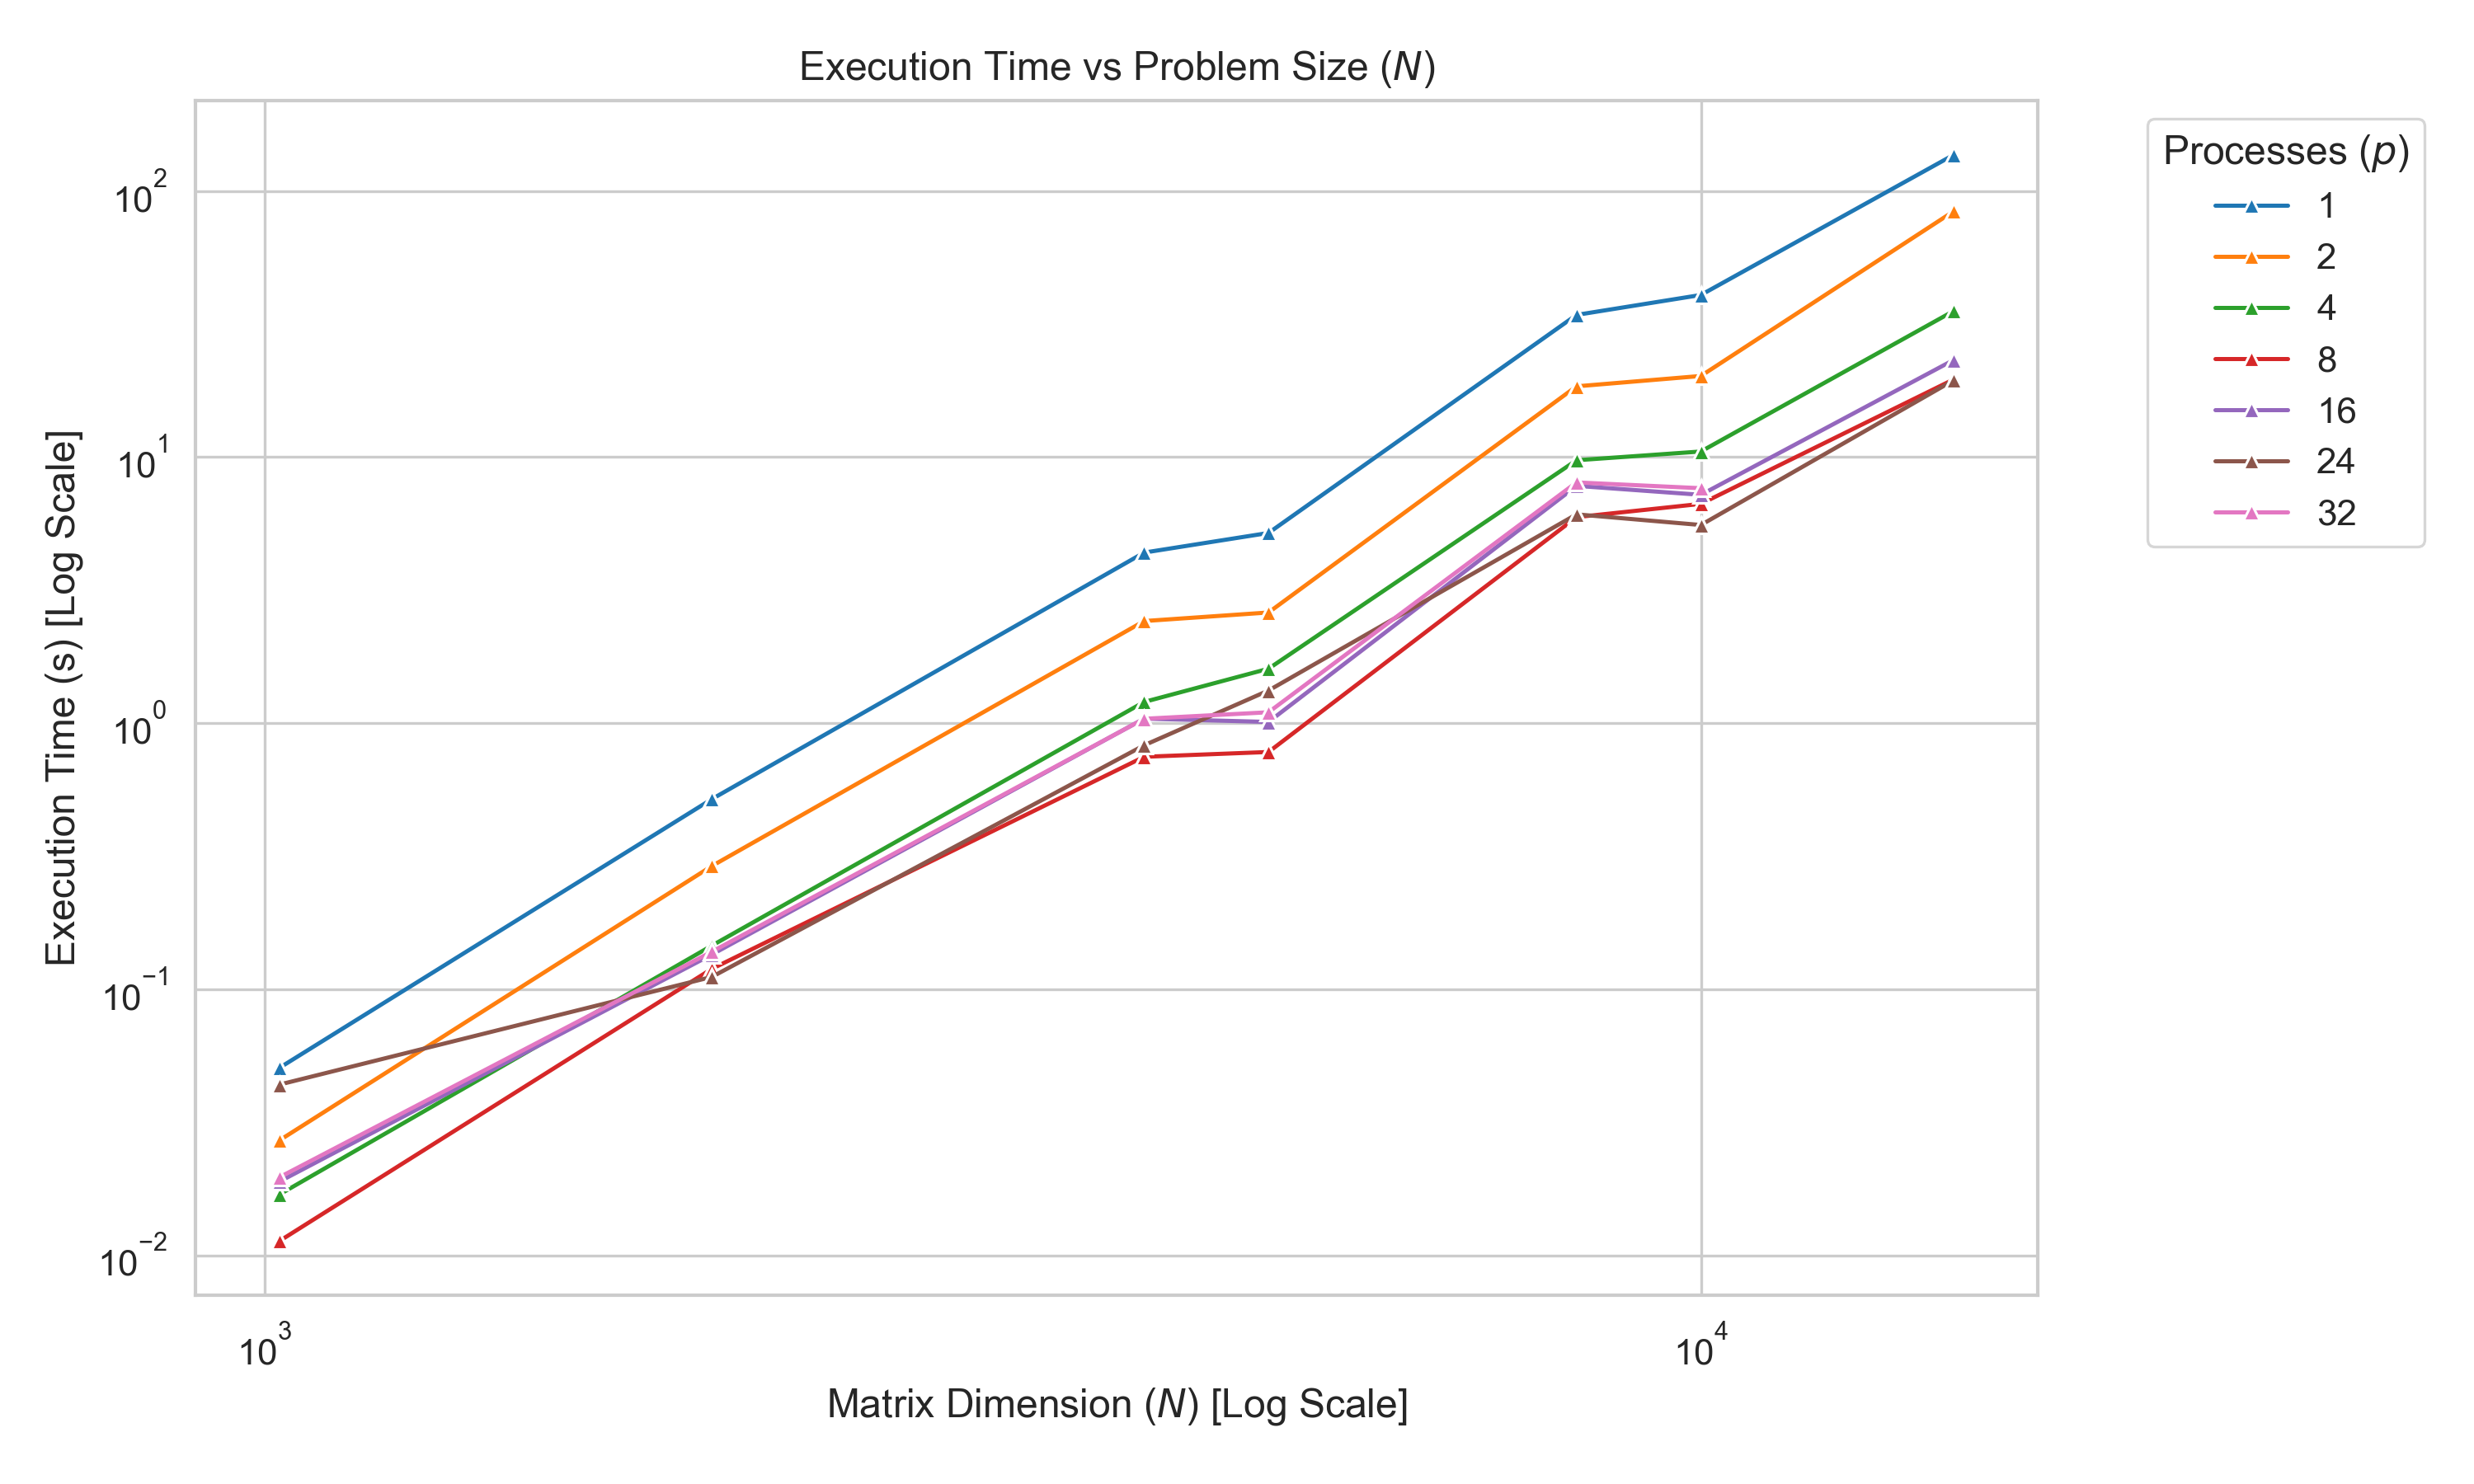
\includegraphics[width=0.8\textwidth]{Images/mpi-plot_5_time_vs_n.png}
    \caption{Execution time compared to problem size $N$ (Log-Log Scale).}
    \label{fig:mpi_time_vs_n}
\end{figure} 

Figure~\ref{fig:mpi_time_vs_n} plots the execution time against the matrix dimension $N$ on a logarithmic scale, perfectly illustrating the theoretical $O(N^3)$ computational complexity of the matrix multiplication algorithm, represented by the consistent positive slope across all process counts.

However, a strict physical limit is reached with $N=15000$ at $p=32$: the independent allocation of matrix $B$ across 32 MPI processes completely saturated the available RAM, causing a runtime Out Of Memory (OOM) error. This highlights the main drawback of MPI on shared-memory architectures compared to OpenMP: severe inefficiency in memory resource utilization.

\subsection{Speedup and Efficiency}

To formally evaluate the implementation, we computed the Speedup ($S_p$) and Efficiency ($E_p$) using the standard formulations $$S_p = T_1 / T_p \qquad and \qquad E_p = S_p / p$$

The speedup plot (Figure~\ref{fig:mpi_speedup}) shows clear sub-linear scaling. For $N = 10000$ at $p=24$, we achieved a maximum speedup of $7.32\times$. For smaller matrices, the communication overhead dominates the computation time almost immediately, leading to a flat speedup curve and a rapidly decreasing efficiency.

\begin{figure}[H]
    \centering
    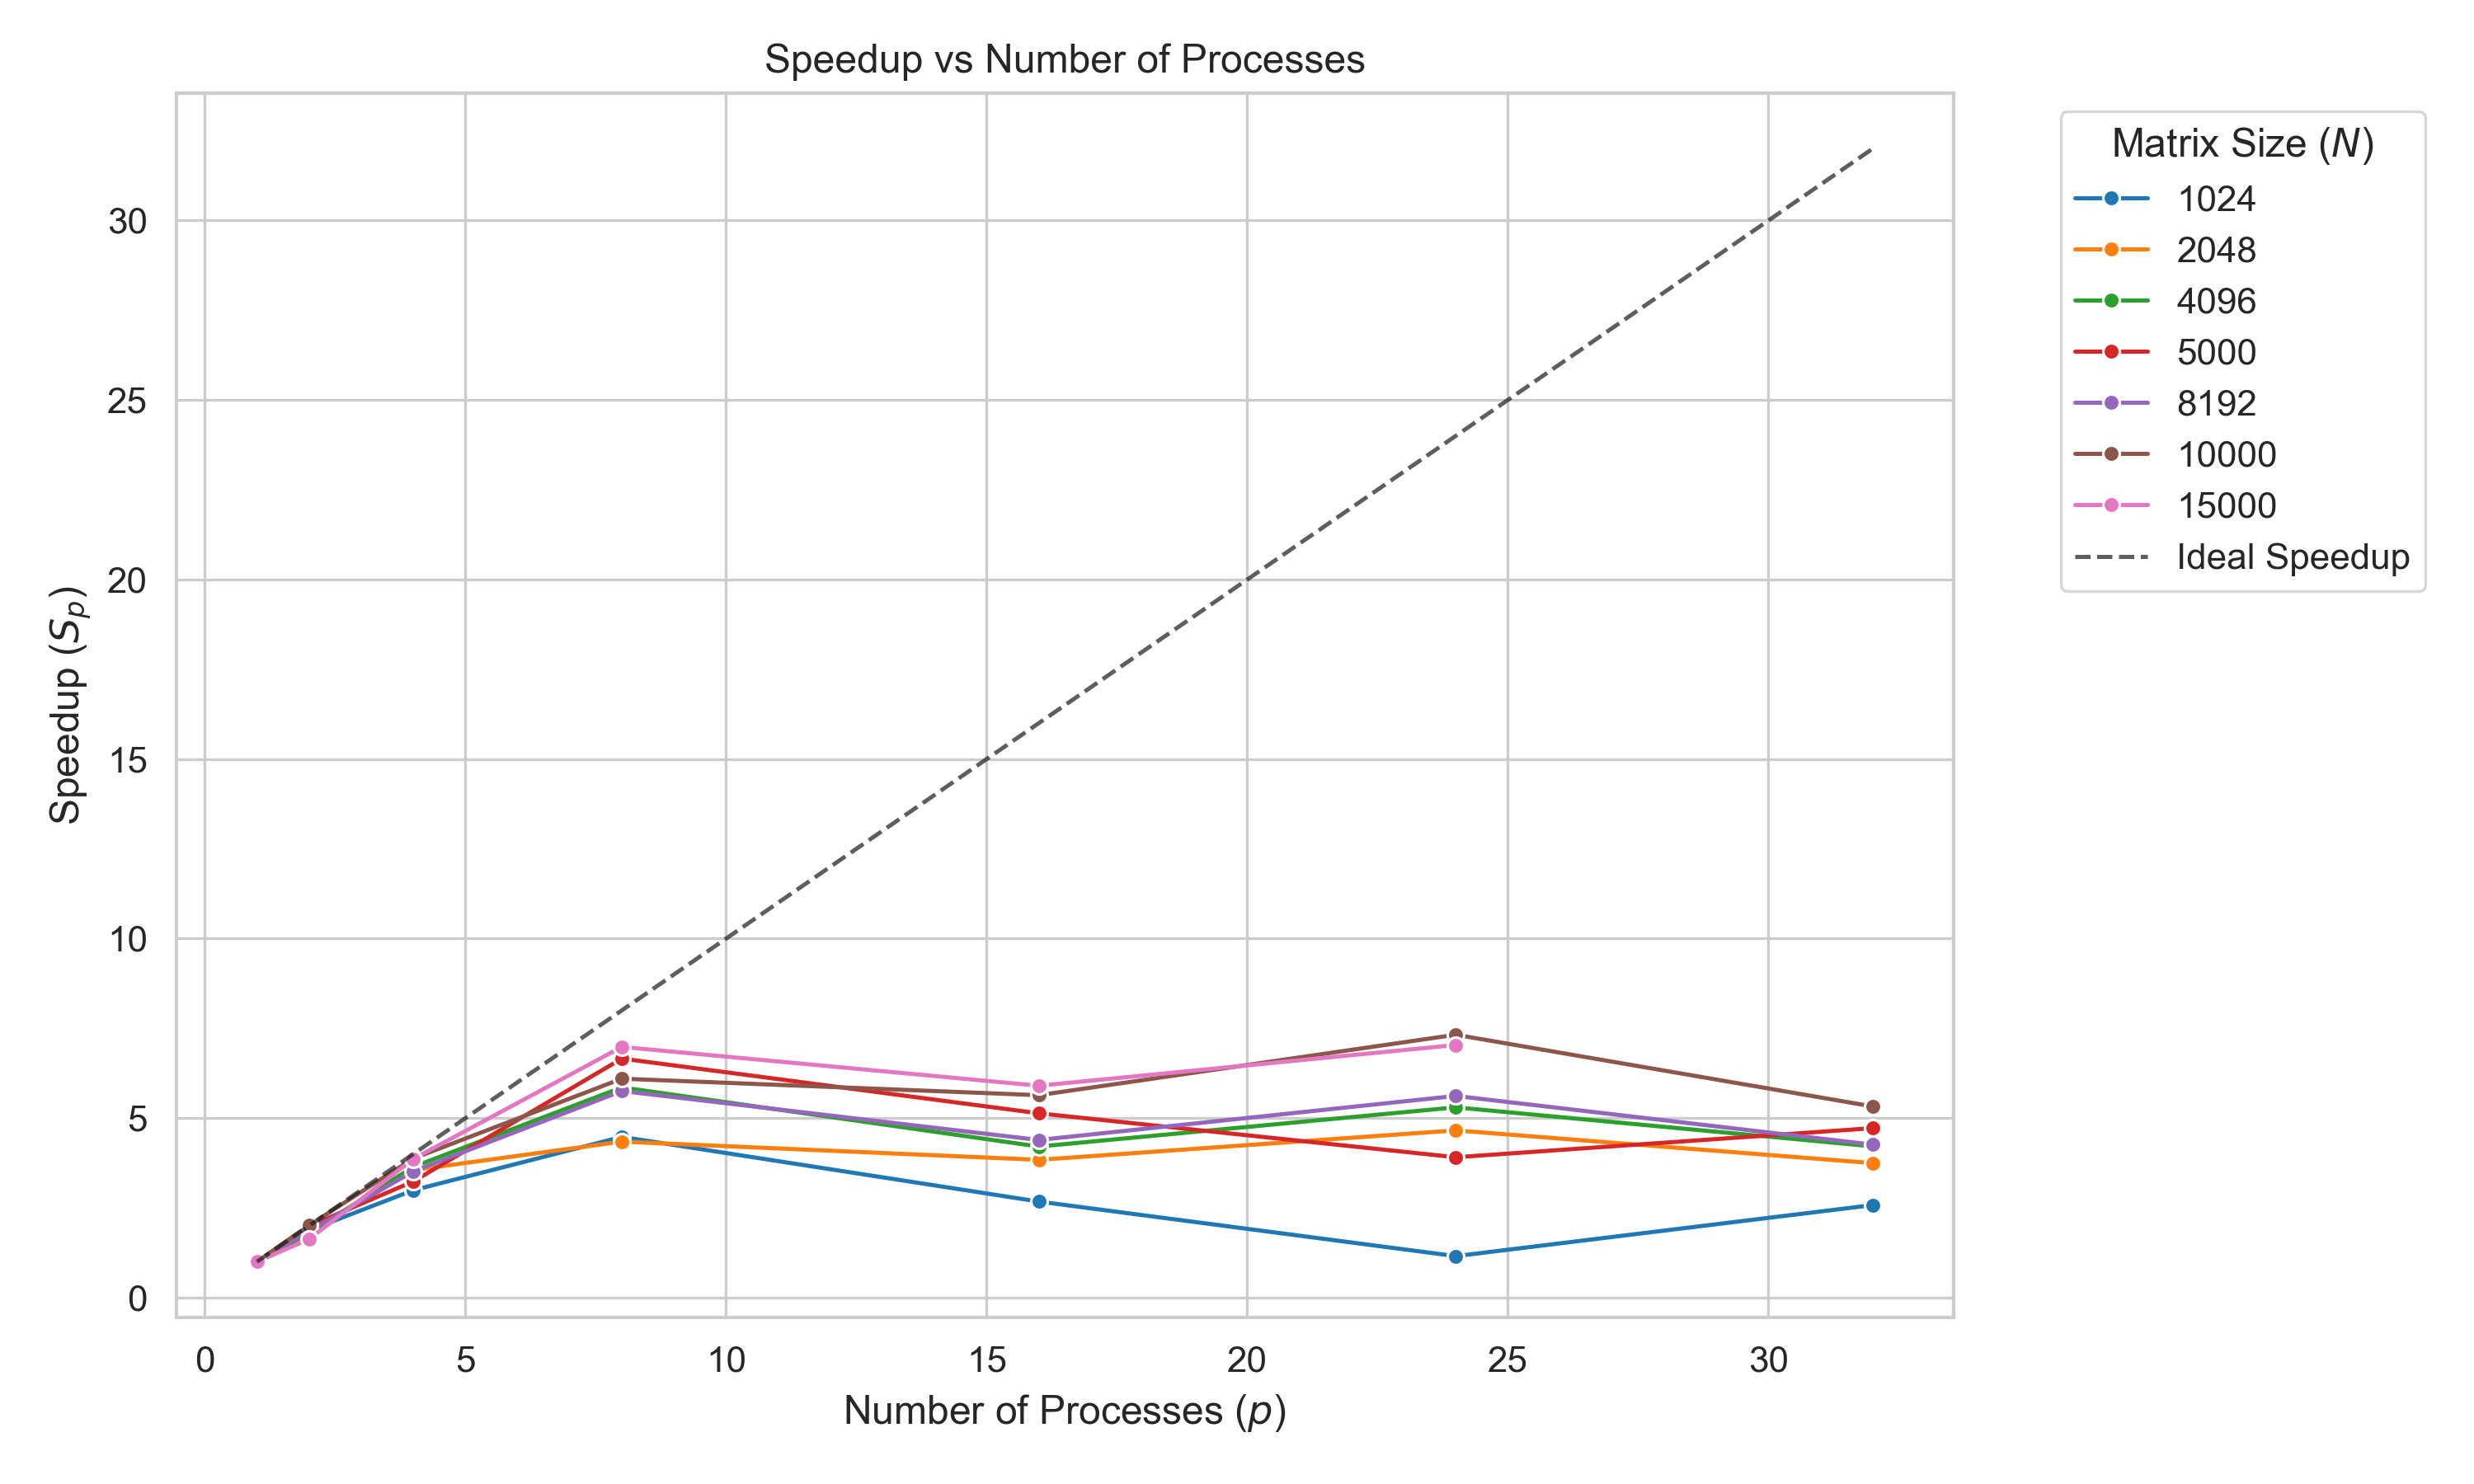
\includegraphics[width=0.8\textwidth]{Images/mpi-plot_2_speedup.png}
    \caption{Speedup compared to number of processes.}
    \label{fig:mpi_speedup}
\end{figure} 

\begin{figure}[H]
    \centering
    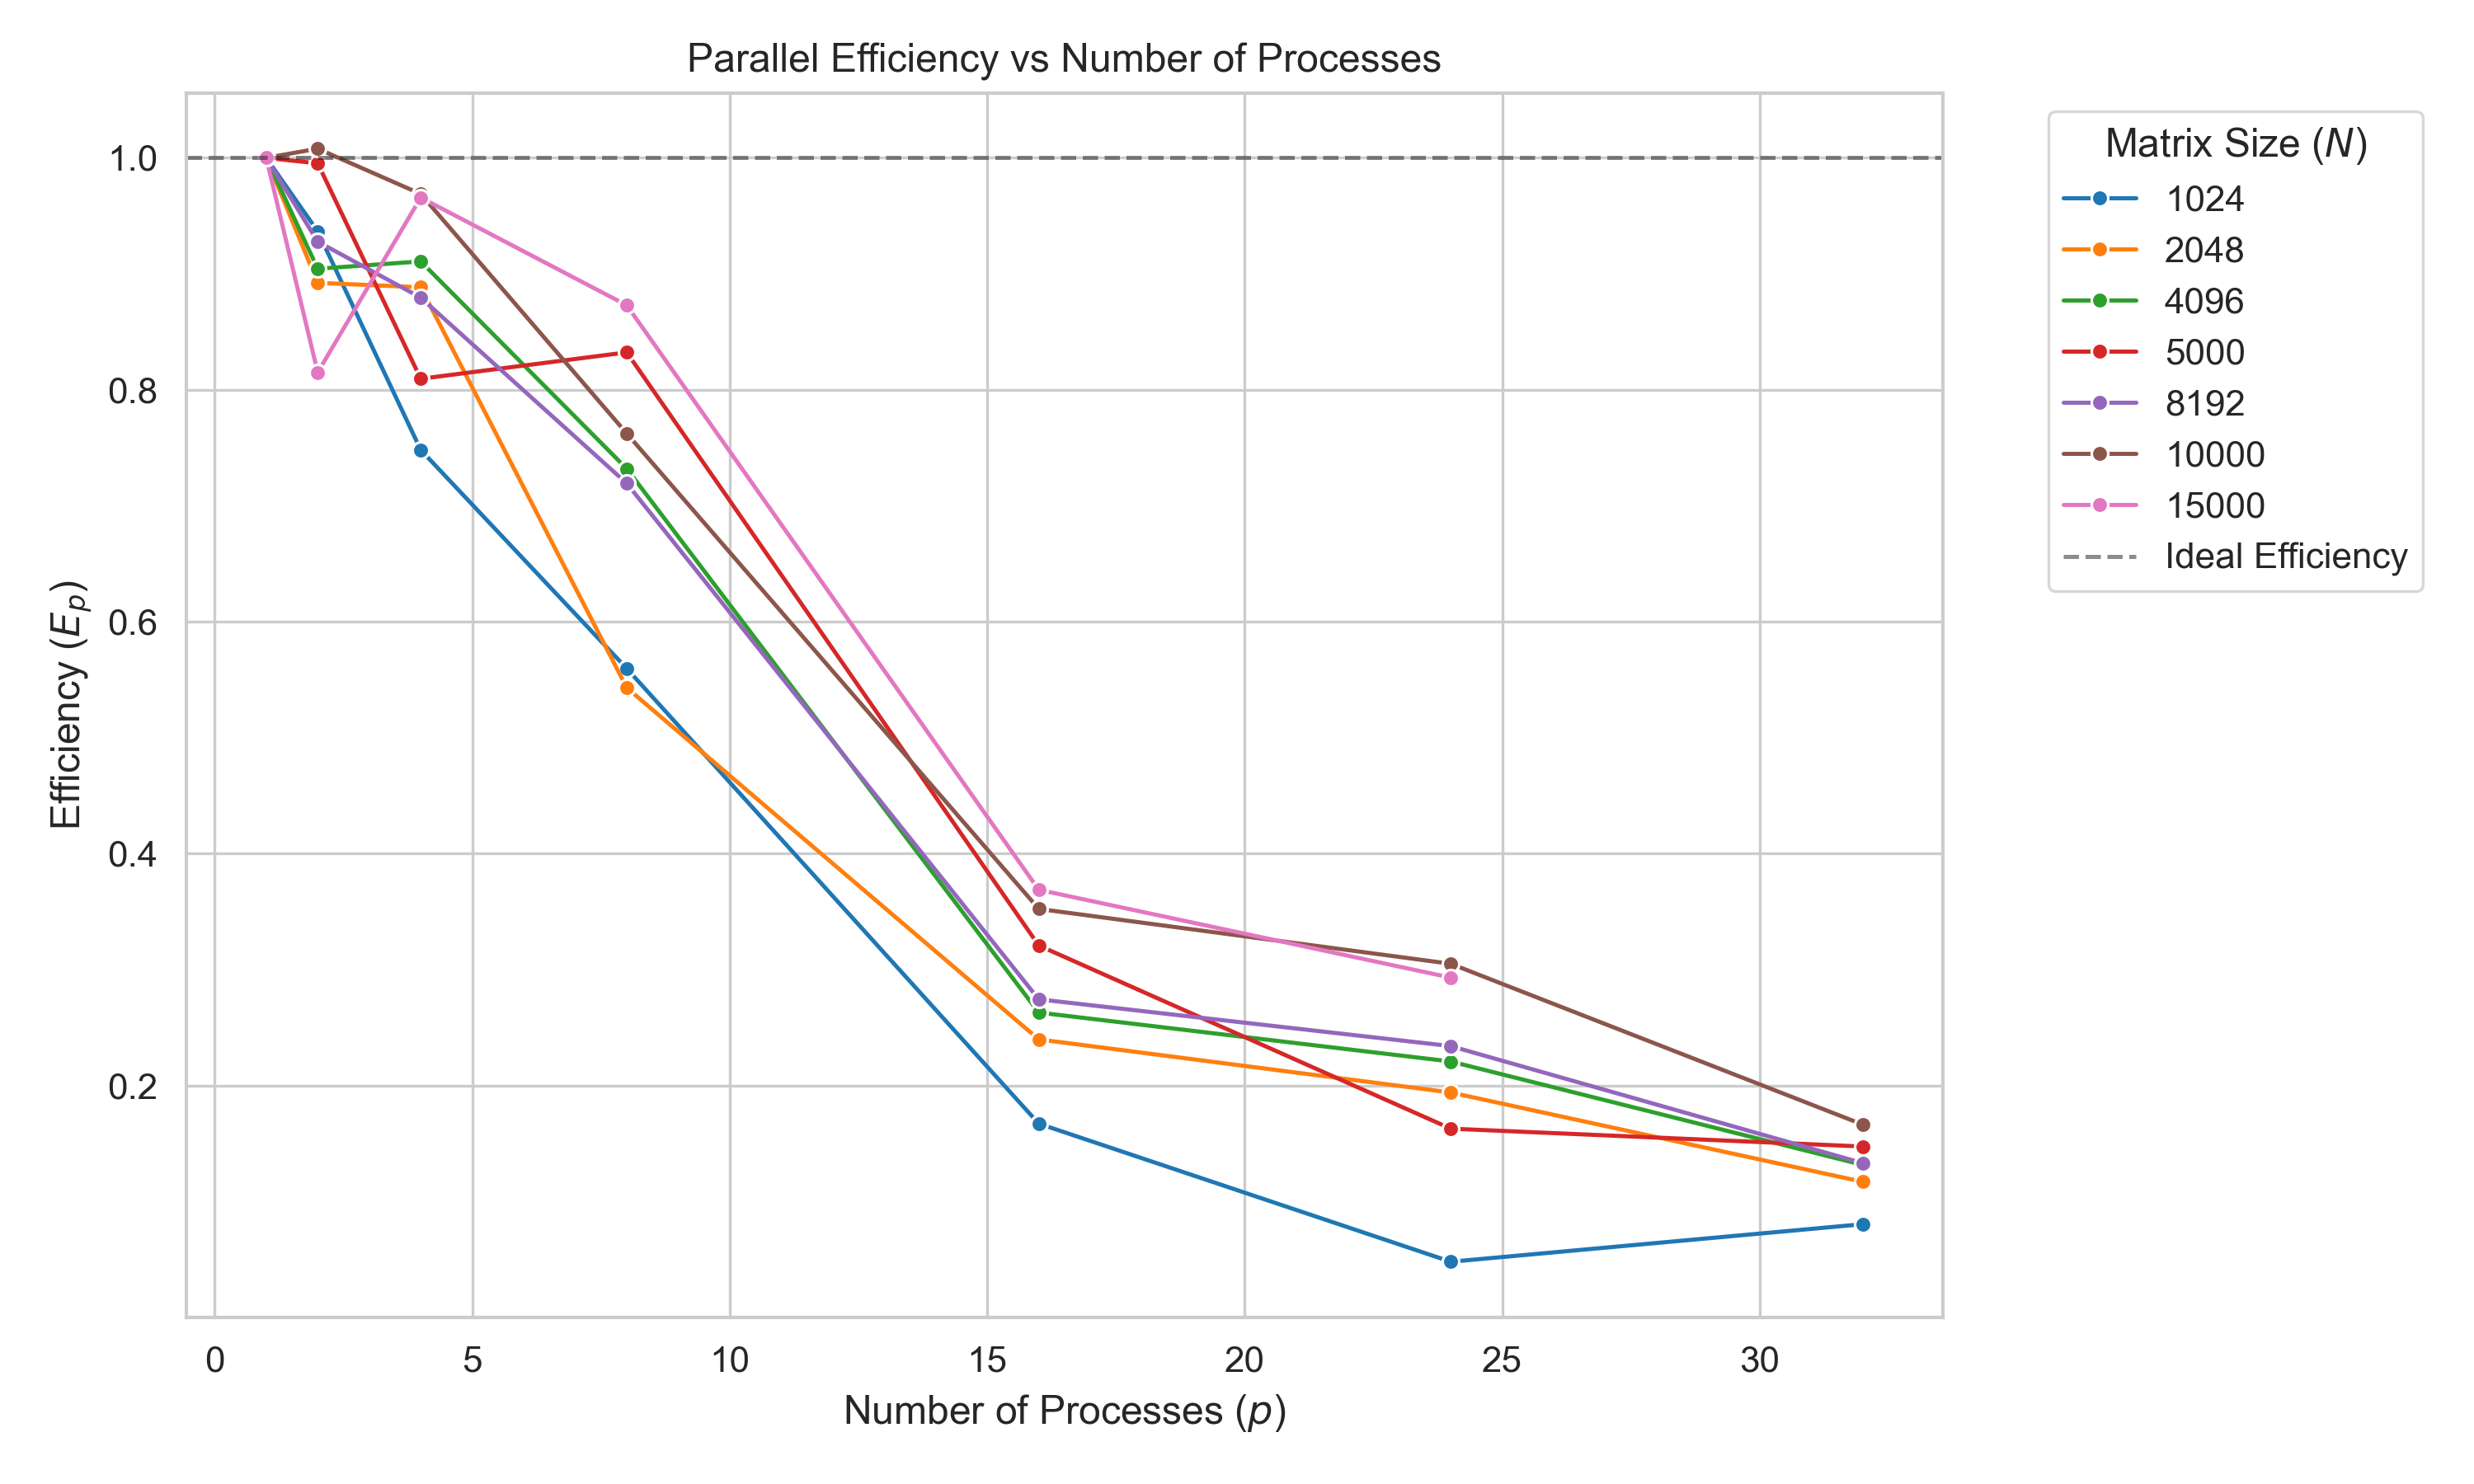
\includegraphics[width=0.8\textwidth]{Images/mpi-plot_3_efficiency.png}
    \caption{Efficiency compared to number of processes.}
    \label{fig:mpi_efficiency}
\end{figure} 

The efficiency heatmap (Figure~\ref{fig:mpi_heatmap}) visualizes the optimal operating window for our MPI implementation. The dark green area indicates that to maintain high efficiency, the problem size can grow but the number of processes must remain "low". When $p$ increases, efficiency drops sharply in the red zone due to inter-process communication dominating execution time.

\begin{figure}[H]
    \centering
    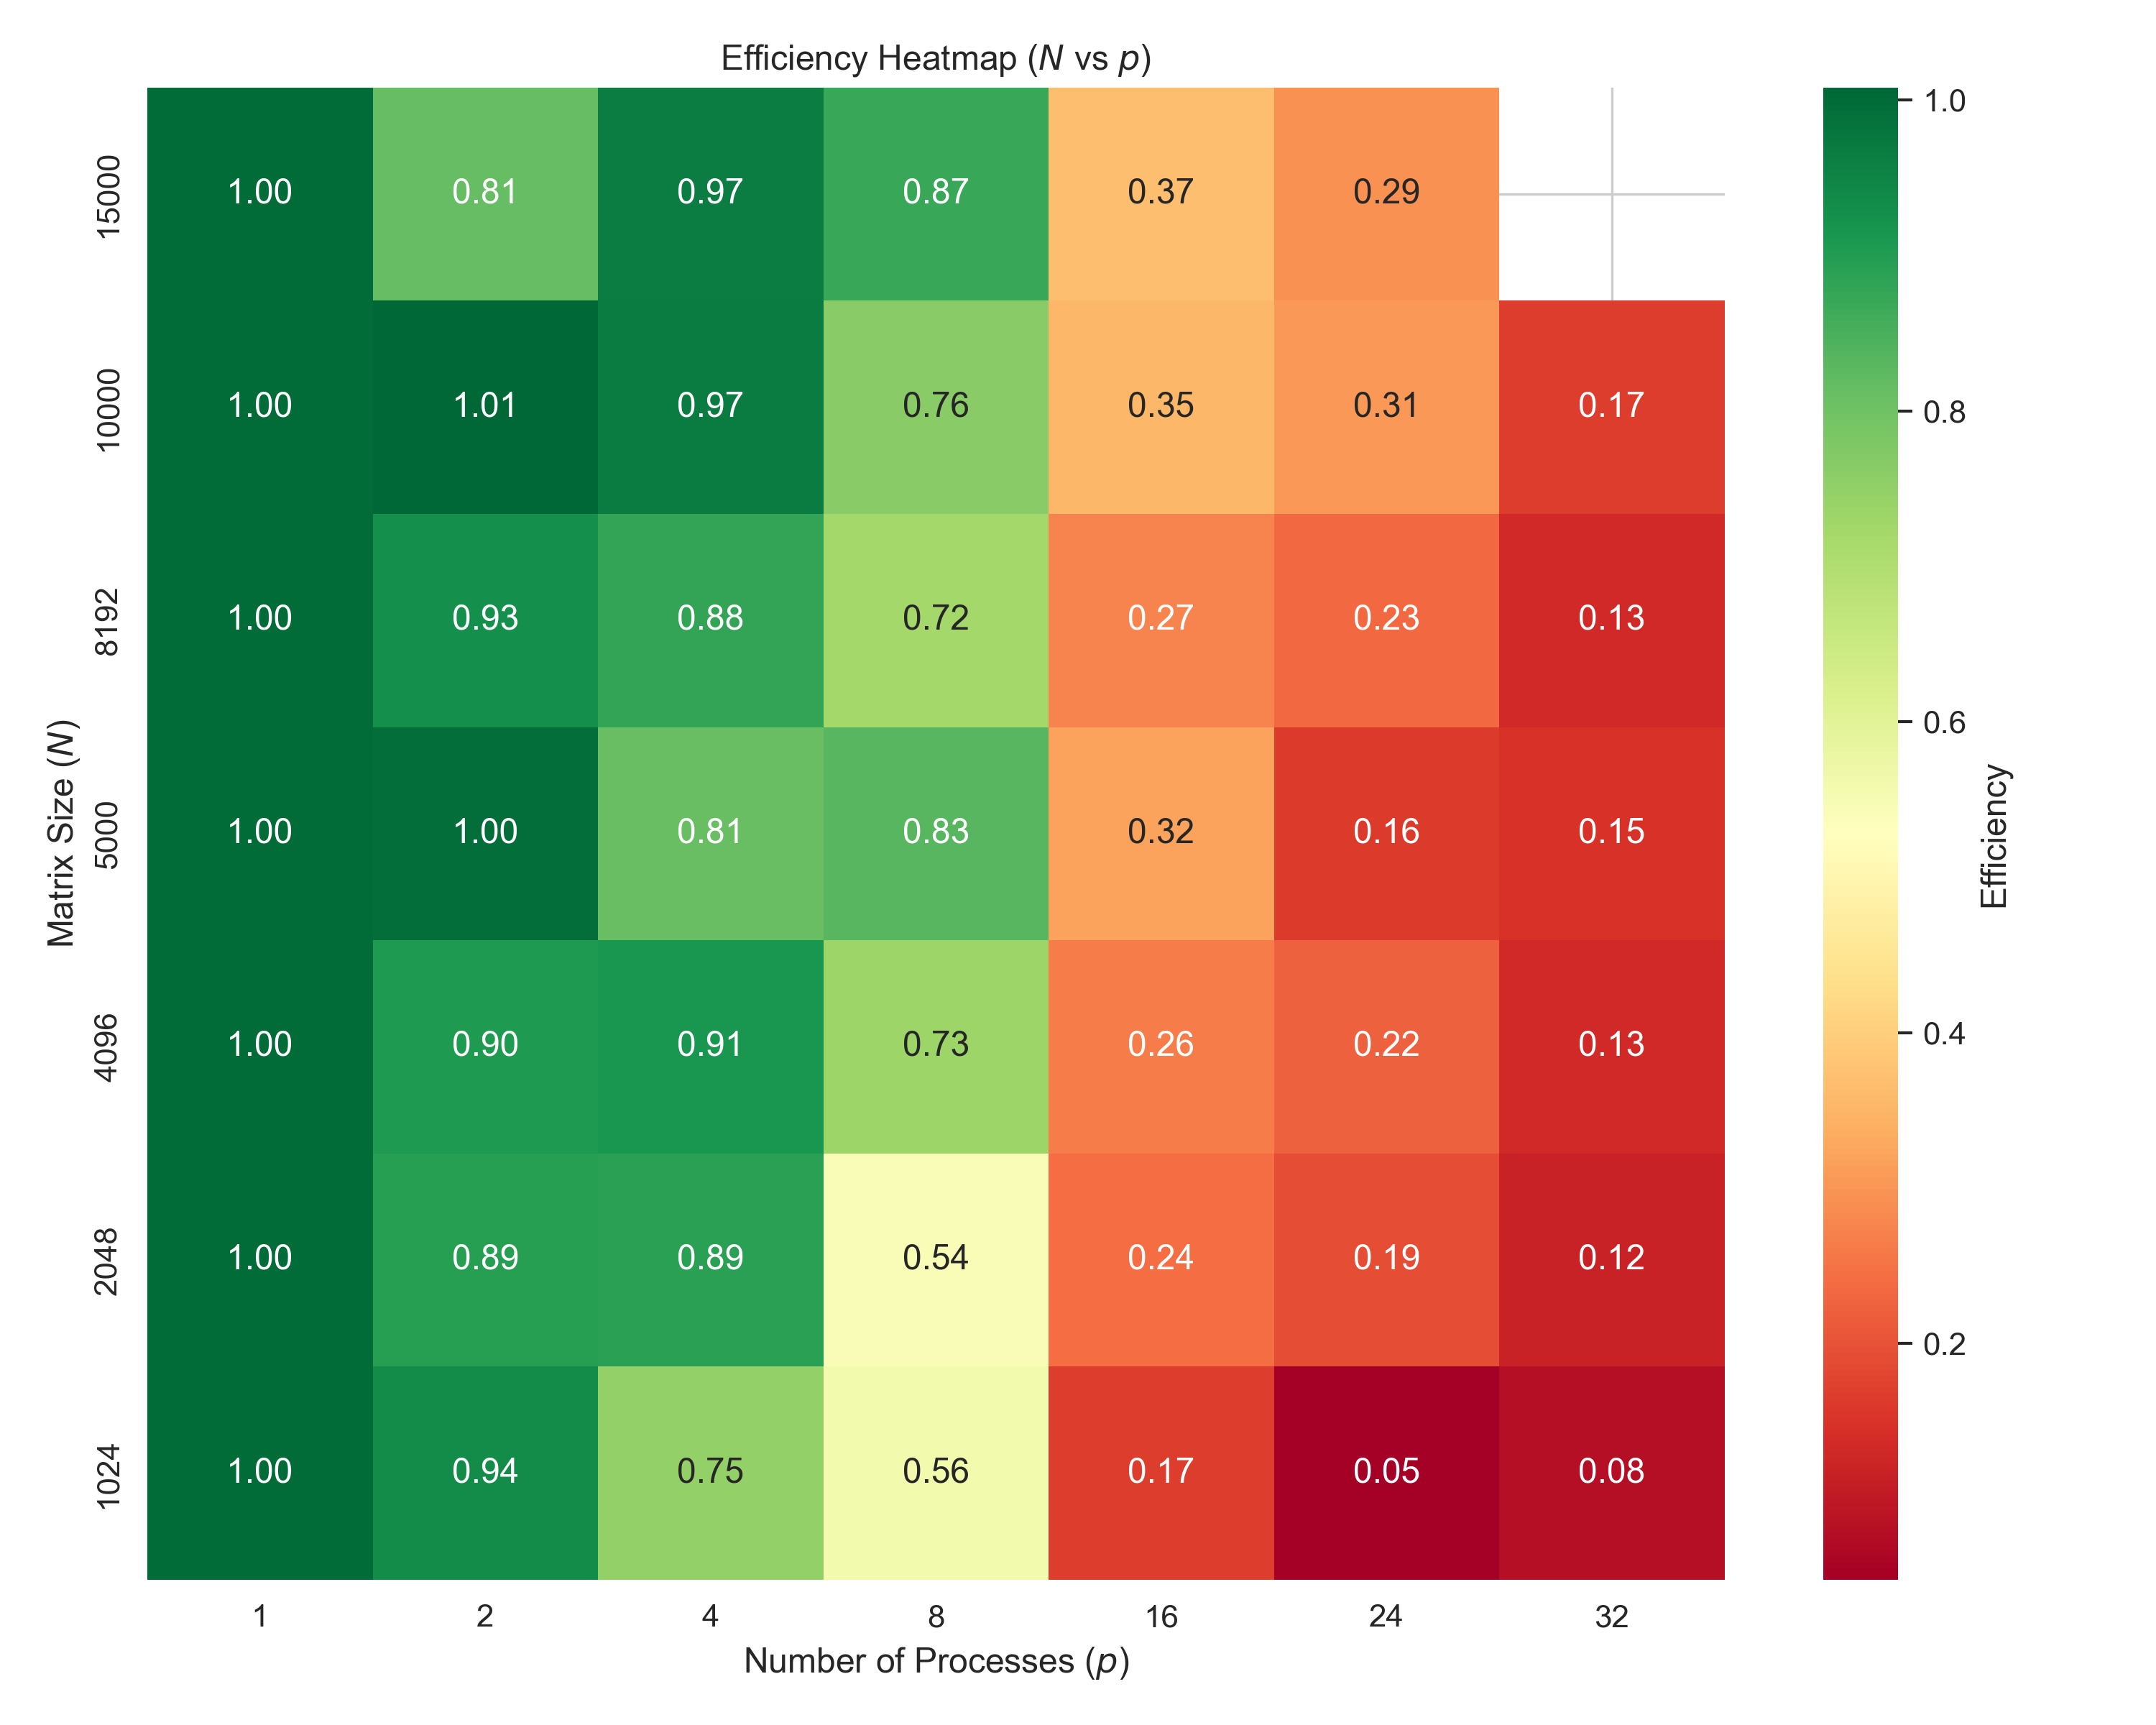
\includegraphics[width=0.75\textwidth]{Images/mpi-plot_6_efficiency_heatmap.png}
    \caption{Efficiency Heatmap mapping the relationship between $N$ and $p$.}
    \label{fig:mpi_heatmap}
\end{figure} 


\subsection{Advanced Throughput and Bottleneck Analysis}

To further assess the hardware utilization and isolate the root causes of the scalability drop, we analyzed the computational throughput and the serial fraction overhead.

\begin{figure}[H]
    \centering
    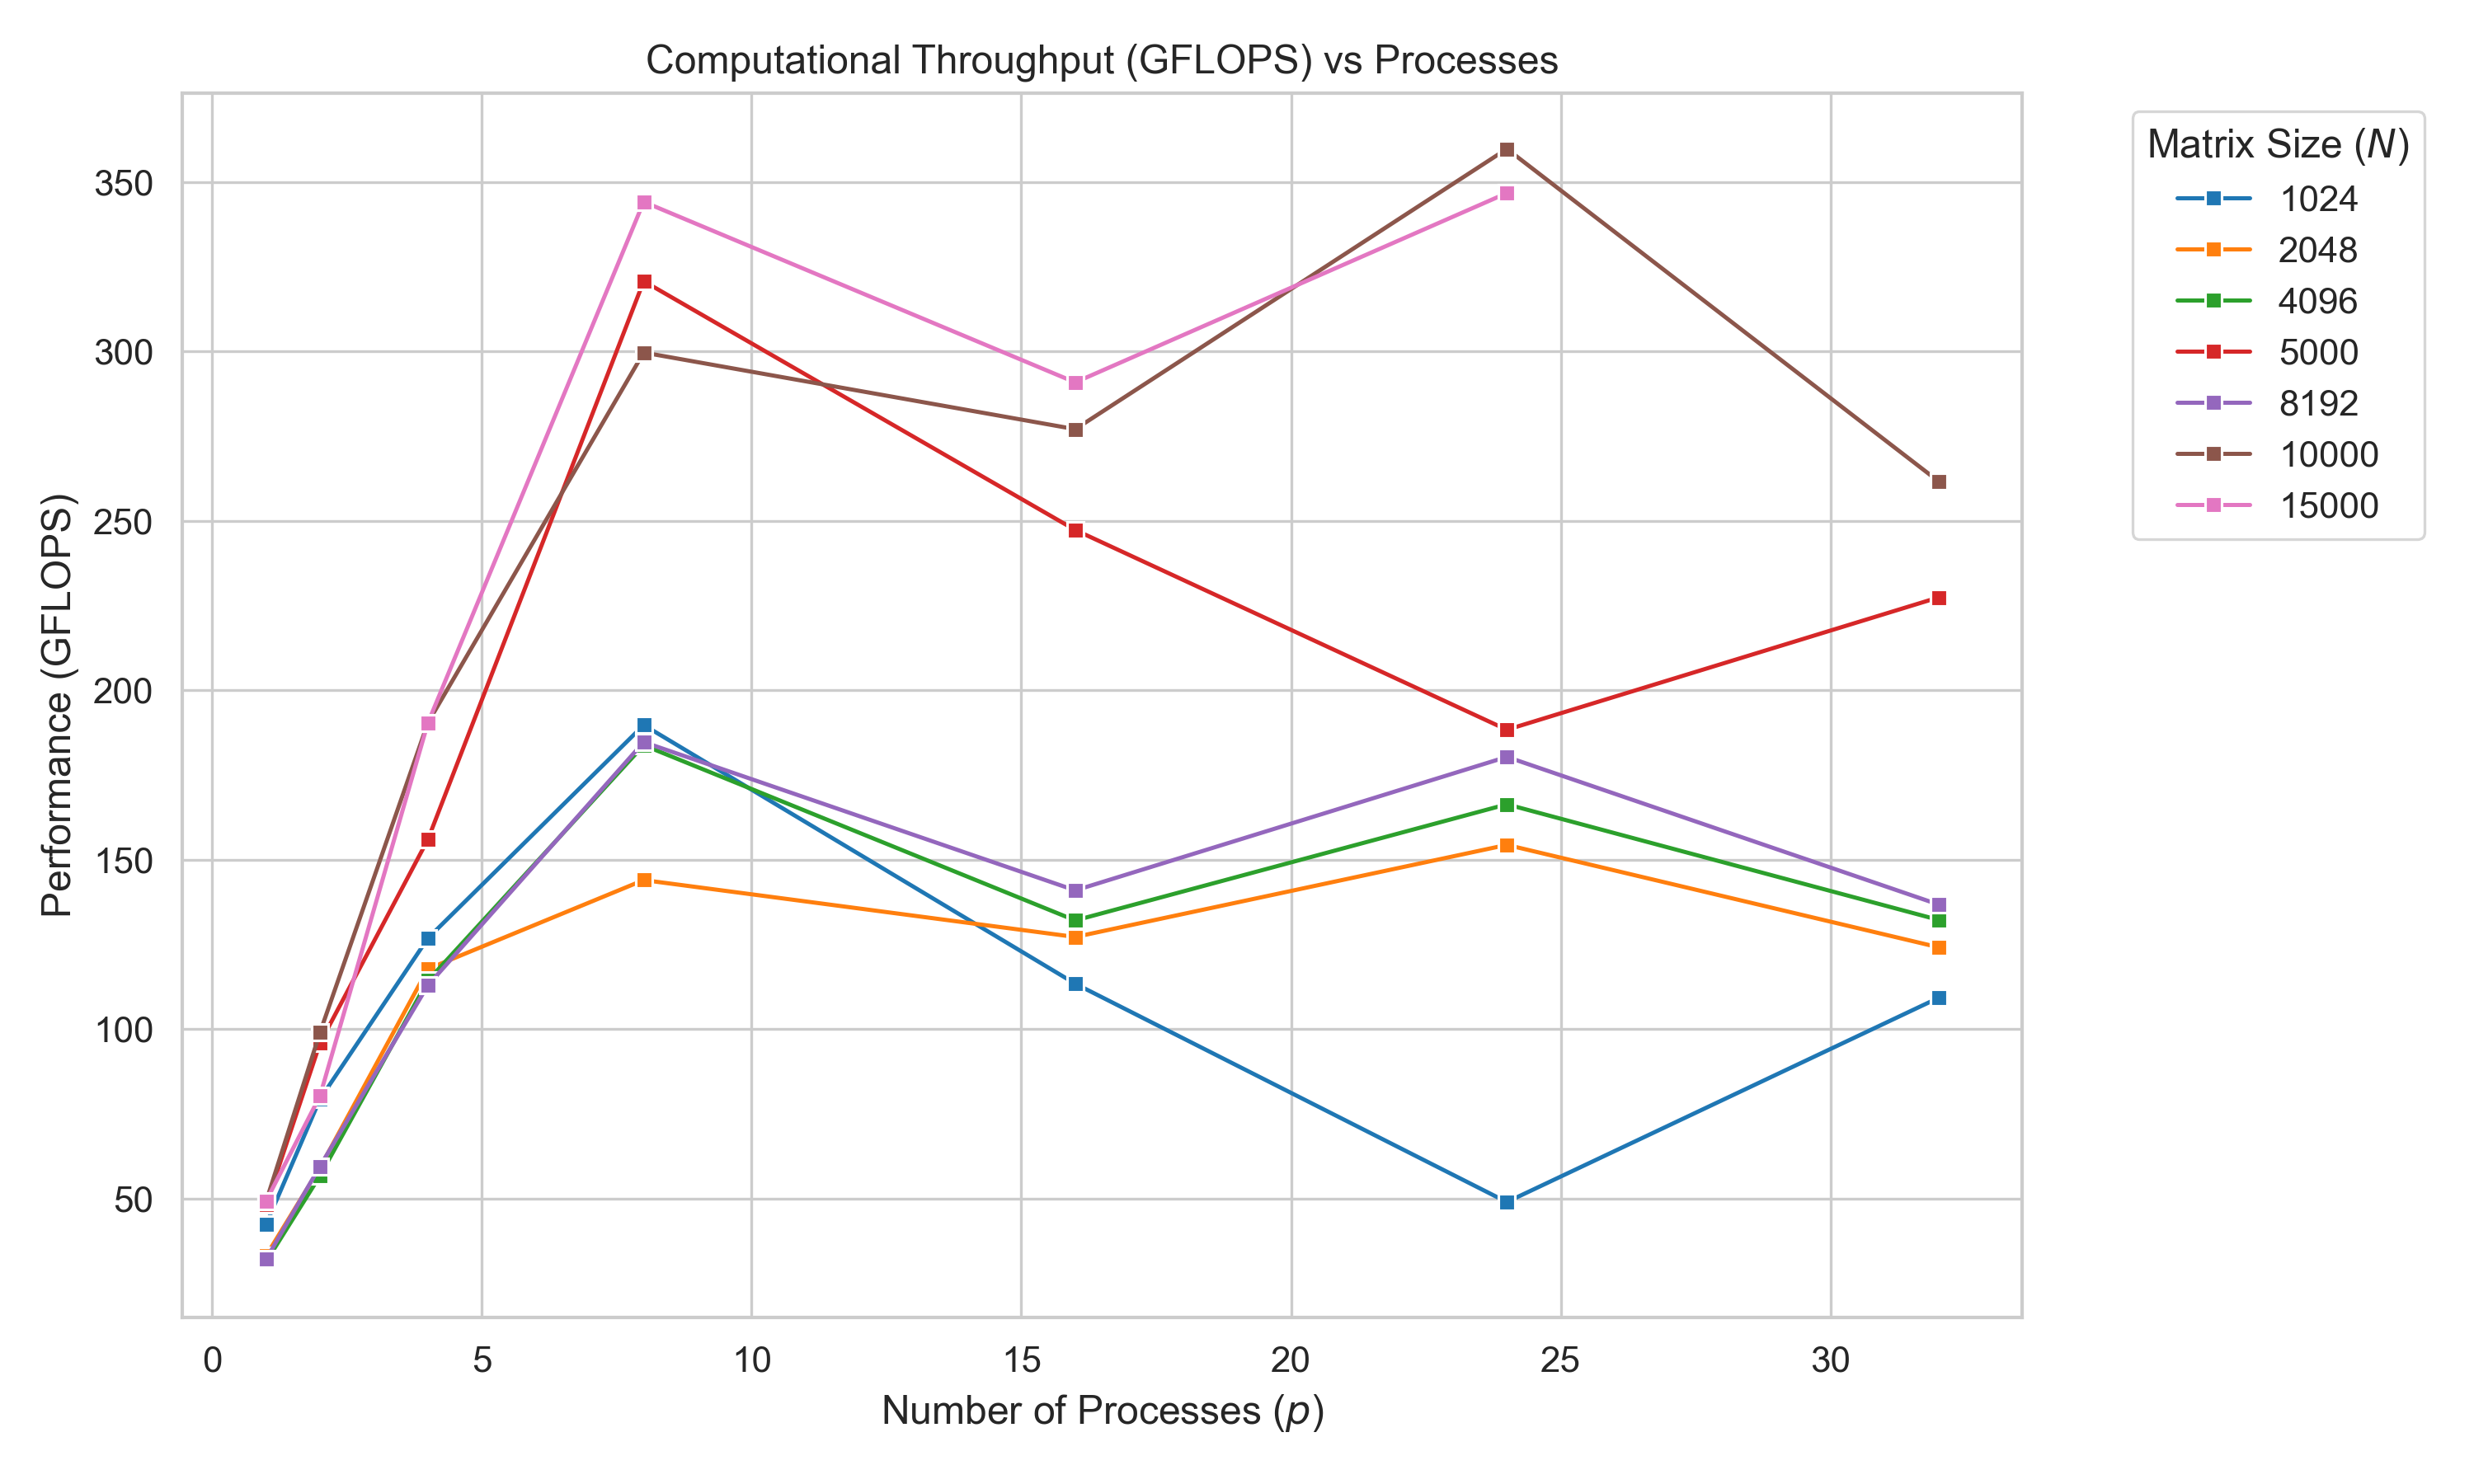
\includegraphics[width=0.8\textwidth]{Images/mpi-plot_4_gflops.png}
    \caption{Computational Throughput (GFLOPS) across different process configurations.}
    \label{fig:mpi_gflops}
\end{figure} 

The GFLOPS chart (Figure~\ref{fig:mpi_gflops}) provides an absolute measure of performance. For small matrices ($N=1024$), the processor barely reaches a few GFLOPS due to constant memory interruption. However, for $N \ge 8192$, the computational throughput scales significantly, demonstrating that the CPU's vector units are being effectively fed with data up until the memory bandwidth saturates.

In conclusion, while the MPI implementation behaves exactly as expected, its deployment on a single machine is definitively bottlenecked by memory bandwidth and data duplication. A physical cluster deployment with high-speed interconnects would be required to mitigate these bounds.

\begin{table}[h!]
\centering
\caption{Complete MPI benchmark results: average execution time (s) across different configurations of processes ($p$) and matrix dimensions ($N$). Note the Out of Memory (OOM) failure for $N=15000$ at $p=32$.}
\label{tab:mpi_final_raw}
\resizebox{\textwidth}{!}{%
\begin{tabular}{@{}lccccccc@{}}
\toprule
\textbf{Configuration} & \textbf{N=1024} & \textbf{N=2048} & \textbf{N=4096} & \textbf{N=5000} & \textbf{N=8192} & \textbf{N=10000} & \textbf{N=15000} \\ \midrule
$p=1$  & 0.0507 & 0.5183 & 4.3779 & 5.1891 & 34.2455 & 40.6978 & 136.9486 \\
$p=2$  & 0.0270 & 0.2904 & 2.4205 & 2.6070 & 18.4566 & 20.1899 & 84.0230 \\
$p=4$  & 0.0169 & 0.1458 & 1.2018 & 1.6025 & 9.7346  & 10.5015 & 35.4518 \\
$p=8$  & 0.0113 & 0.1193 & 0.7476 & 0.7794 & 5.9511  & 6.6733  & 19.6115 \\
$p=16$ & 0.0189 & 0.1350 & 1.0403 & 1.0108 & 7.7987  & 7.2178  & 23.2034 \\
$p=24$ & 0.0438 & 0.1113 & 0.8260 & 1.3271 & 6.0952  & \textbf{5.5584} & \textbf{19.4649} \\
$p=32$ & 0.0197 & 0.1383 & 1.0390 & 1.0992 & 8.0357  & 7.6417  & \text{ERROR} \\ \midrule
\textbf{Optimized (MKL)*} & \textit{\textasciitilde 0.005} & \textit{\textasciitilde 0.04} & \textit{\textasciitilde 0.32} & \textit{\textasciitilde 0.45} & \textit{\textasciitilde 2.5} & \textit{\textasciitilde 4.5} & \textit{\textasciitilde 15.0} \\ \bottomrule
\end{tabular}%
}
\par\smallskip
\small *Theoretical performance estimation using Intel MKL/ScaLAPACK libraries with AVX-512 instructions.
\end{table}

\newpage
\section{Final Comparison}\label{sec:results}

For completeness, Table~\ref{table:results} provides an integral summary of the best performances achieved across all our implementations, illustrating the overall optimization trajectory for matrices of the tested dimensions.

\begin{table}[H]
\centering
% The resizebox must wrap the ENTIRE threeparttable
\resizebox{\textwidth}{!}{%
  \begin{threeparttable}
    \caption{Integral performance summary of all implementations across matrix dimensions $N=5000$, $10000$, and $15000$. Percentages reflect computational throughput (GFLOPS) relative to the best measured baseline: Intel MKL (OpenMP, $T=16$).}
    \label{table:results}
    
    \begin{tabular}{l|ccc|ccc|ccc}
    \toprule
     & \multicolumn{3}{c|}{\textbf{N = 5000}} & \multicolumn{3}{c|}{\textbf{N = 10000}} & \multicolumn{3}{c}{\textbf{N = 15000}} \\
    \textbf{Implementation} & \textbf{Time (s)} & \textbf{GFLOPS} & \textbf{\%} & \textbf{Time (s)} & \textbf{GFLOPS} & \textbf{\%} & \textbf{Time (s)} & \textbf{GFLOPS} & \textbf{\%} \\
    \midrule

    \multicolumn{10}{c}{\textbf{Sequential Implementations}} \\
    \midrule
    ICC \texttt{-O0}                         & 388.781 & 0.64  & 0.14\%  & 3028.552 & 0.66  & 0.13\%  & - & - & - \\
    ICC \texttt{-O1}                         & 69.403  & 3.60  & 0.77\%  & 525.154  & 3.81  & 0.73\%  & - & - & - \\
    ICC \texttt{-O2}                         & 50.030  & 5.00  & 1.07\%  & 401.861  & 4.98  & 0.96\%  & - & - & - \\
    ICC \texttt{-O3}                         & 18.258  & 13.69 & 2.94\%  & 196.361  & 10.19 & 1.96\%  & - & - & - \\
    ICC \texttt{-O3 -xHost}\tnote{1}         & 9.901   & 25.25 & 5.42\%  & 70.019   & 28.56 & 5.51\%  & 275.428 & 24.51 & 4.69\% \\
    ICC \texttt{-O3 -xHost}\tnote{1} \texttt{-DALIGN} & 6.511   & 38.40 & 8.24\%  & 52.206   & 38.31 & 7.39\%  & 175.374 & 38.49 & 7.37\% \\
    Custom OpenBLAS (Seq)                    & 4.556   & 54.87 & 11.78\% & 36.864   & 54.25 & 10.46\% & 123.927 & 54.47 & 10.43\% \\
    OpenBLAS (Seq)                           & 4.406   & 56.74 & 12.18\% & 32.458   & 61.62 & 11.88\% & 109.035 & 61.91 & 11.85\% \\
    Intel MKL (Seq)                          & 4.020   & 62.19 & 13.35\% & 32.076   & 62.35 & 12.02\% & 108.020 & 62.49 & 11.97\% \\
    
    \midrule
    \multicolumn{10}{c}{\textbf{OpenMP Implementations}} \\
    \midrule
    Original ($T=24$)                        & 5.360 & 46.65 & 10.02\% & 43.087 & 46.42 & 8.95\%  & 149.783 & 45.07 & 8.63\% \\
    Blas-Like ($T=16$, default)              & 0.837 & 298.62 & 64.11\% & 5.789 & 345.47 & 66.62\% & 16.752 & 402.93 & 77.15\% \\
    Blas-Like ($T=16$, dynamic, 1)           & 0.804 & 310.97 & 66.76\% & 4.977 & 401.82 & 77.49\% & 15.571 & 433.49 & 83.01\% \\
    Blas-Like (Optimal)\tnote{2}             & 0.882 & 283.32 & 60.83\% & 4.906 & 407.67 & 78.61\% & 15.571 & 433.50 & 83.01\% \\
    OpenBLAS ($T=16$)                        & 0.662 & 377.37 & 81.02\% & 4.677 & 427.65 & 82.47\% & 16.997 & 397.13 & 76.04\% \\
    \textbf{Intel MKL ($T=16$)}              & \textbf{0.537} & \textbf{465.77} & \textbf{100.00\%} & \textbf{3.857} & \textbf{518.57} & \textbf{100.00\%} & \textbf{12.925} & \textbf{522.24} & \textbf{100.00\%} \\

    \midrule
    \multicolumn{10}{c}{\textbf{CUDA Implementations}} \\
    \midrule
    Kernel 1 (16x16)                         & 1.600 & 156.25 & 33.55\% & 11.034 & 181.26 & 34.95\% & 42.411 & 159.16 & 30.48\% \\
    Kernel 2 (32x32)                         & 1.411 & 177.18 & 38.04\% & 9.973  & 200.54 & 38.67\% & 33.582 & 201.00 & 38.49\% \\
    cuBLAS                                   & 1.326 & 188.54 & 40.48\% & 8.921  & 224.19 & 43.23\% & 29.304 & 230.34 & 44.11\% \\

    \midrule
    \multicolumn{10}{c}{\textbf{MPI Implementations}} \\
    \midrule
    MPI Original($p=24$)                             & 1.327 & 188.38 & 40.44\% & 5.558  & 359.82 & 69.39\% & 19.465 & 346.78 & 66.40\% \\
    MPI Intel MKL\tnote{3}                & \textit{\textasciitilde 0.450} & \textit{555.56} & \textit{119.28\%} & \textit{\textasciitilde 4.500} & \textit{444.44} & \textit{85.70\%} & \textit{\textasciitilde 15.000} & \textit{450.00} & \textit{86.17\%} \\
    
    \bottomrule
    \end{tabular}
    
    \begin{tablenotes}
        \footnotesize
        \item[1] Actually were also used \texttt{-ipo}, \texttt{-fp-model}, \texttt{fast=2}, \texttt{-fno-alias}, \texttt{-inline-level=2}, \texttt{-unroll-aggressive}, \texttt{-unroll=4}, as explained in Table~\ref{tab:advanced_flags}.
        \item[2] Evaluated with tuned affinity settings: \texttt{OMP\_PROC\_BIND=close, OMP\_PLACES=sockets}.
        \item[3] Theoretical performance estimation using Intel MKL/ScaLAPACK libraries with AVX-512 instructions.
    \end{tablenotes}
  \end{threeparttable}%
}
\end{table}

\newpage
\begin{appendices}
\section{Sequential Algorithms}\label{app:algorithms}
The progressive optimization of matrix multiplication relies heavily on understanding how modern hardware manages memory. This section details the theoretical and practical logic behind the sequential algorithms evaluated, illustrating the shift from a direct mathematical translation to a highly optimized, hardware-aware implementation.


\subsection{Naive Approach: $i-j-k$}\label{subsec:ijk}

The standard triple-nested loop represents the most intuitive translation of the mathematical definition of matrix multiplication. For square matrices A and B, the product matrix C is defined as:

$$C_{ij}=\sum_{k=1}^{n}A_{ik}\cdot B_{kj}$$

To compute a single element $C_{ij}$, the algorithm calculates the complete dot product between the $i$-th row of matrix A and the $j$-th column of matrix B. 
While mathematically sound, this approach is highly inefficient for large matrices: because the innermost loop iterates over $k$, the algorithm accesses the elements of $B_{kj}$ by jumping across distinct rows in memory. 

In standard C-style row-major memory layouts, this column-wise traversal breaks the \emph{spatial locality} exploited by the caching: it forces the CPU to continuously fetch new cache lines from main memory, leading to poor cache utilization and significant execution stalls.

Note that this implementation performs so badly that it is not even cited in this report, that starts directlyu with  the next approach

\subsection{Standard Approach: $i-k-j$}\label{subsec:ikj}

To address the severe memory inefficiencies of the naive implementation, the standard optimization involves a simple structural adjustment: swapping the order of the inner loops to $i-k-j$. Reordering the loops fundamentally changes the sequence of the arithmetic operations without altering the final mathematical result. Instead of calculating a single element $C_{ij}$ to completion, this approach takes a scalar element $A_{ik}$ and multiplies it across the entire $k$-th row of B, accumulating those partial results into the $i$-th row of C.

The innermost loop executes as follows:
\begin{verbatim}
for (int j = 0; j < n; j++)
    C[i][j] += A[i][k] * B[k][j];
\end{verbatim}

By making $j$ the innermost loop, the algorithm ensures that both matrix C and matrix B are accessed in a linear fashion: as $j$ increments, the memory addresses requested are strictly sequential. 

This continuous row-major traversal takes full advantage of spatial locality and hardware prefetching mechanisms, keeping the CPU pipelines fed and drastically reducing overall memory latency.

\subsection{Better Approach: Tiling (Blocking)}\label{subsec:tiling}


While the $i-k-j$ approach successfully linearizes access, its performance degrades when the active working set exceeds the capacity of the CPU's cache hierarchy. If the matrices are large enough, an entire row may be evicted from the cache before the algorithm can return to reuse it in the next iteration. Loop tiling (also known as blocking) directly addresses this limitation.

\begin{figure}[H]
    \centering
    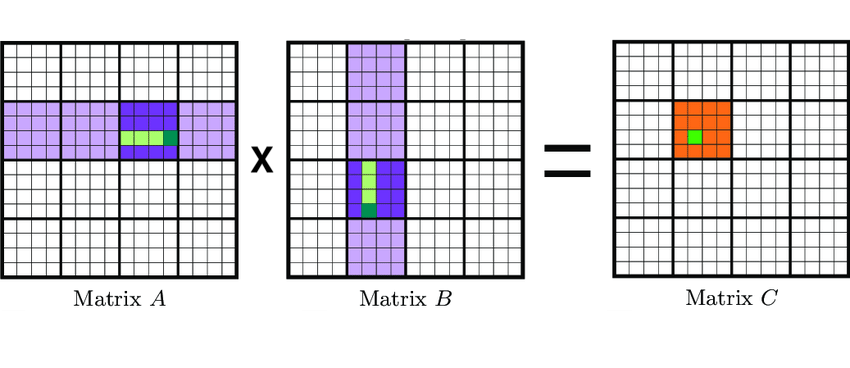
\includegraphics[width=0.8\linewidth]{appendices/tiling.png}
    \caption{Loop decomposition to allow for Explicit Tiling}
    \label{fig:tiling_image}
\end{figure}

Tiling decomposes the standard n-depth loop nest into a more complex, deeply nested structure : it partitions the vast iteration space into smaller, fixed-size geometric blocks, or tiles. By restricting the active computation to a specific tile, the compiler effectively limits the kernel's active working set. 

This methodology prevents the \textbf{cache thrashing} typical of naive matrix multiplication, where data is evicted before it can be reused in the next outer-loop iteration. Because the data blocks remain resident in the cache for the duration of the tile's computation, the algorithm maximizes temporal locality and avoids the massive latency penalty of repeatedly fetching data from main memory.

This implementation can be exploited by the compiler in a autonomous way, as  we have addressed in Subsection~\ref{subsec:seq_3}; nonetheless the explicit partitioning in "working sets" still suffer from the \emph{cache-associativity} problem, hence it requires further optimizations.

\subsection{Best implementation: \texttt{OpenBlas} }\label{subsec:openblas}

While standard loop tiling ensures that active matrix blocks fit within the CPU's cache, it does not solve the fundamental issue of memory continuity. Because the original matrices $A$ and $B$ are allocated in a standard row-major layout, a two-dimensional tile extracted directly from them still consists of fragmented memory segments: jumping across these non-contiguous rows inside the cache can trigger associative cache collisions and memory stalls. 

To approach peak theoretical hardware limits, we must abandon in-place computation and adopt explicit data packing strategies characteristic of the OpenBLAS/BLIS architecture.

\begin{figure}[H]
\centering
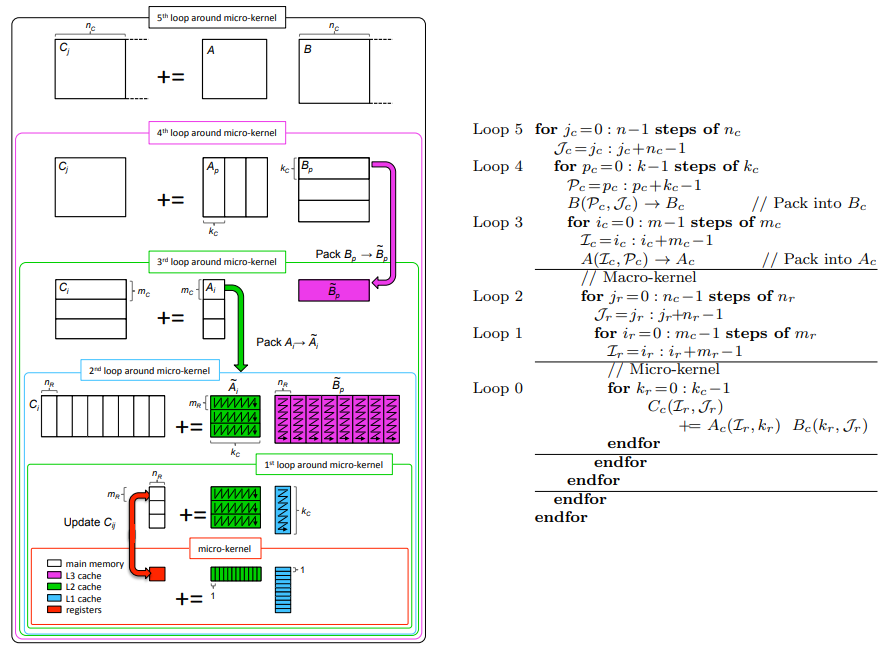
\includegraphics[width=1\textwidth]{appendices/blas.png}
\caption{Schematic Blueprint of the OpenBlas approach}
\label{fig:blas}
\end{figure}

\subsubsection{Memory Packing (Macro-Kernel Logic)}
The foundation of this architecture is the deliberate reorganization of the working set into perfectly contiguous memory buffers before any math is performed. Instead of reading directly from the global row-major matrices during the arithmetic operations, the outer loops (often called the ``macro-kernel'') extract sub-matrices and pack them into custom linear arrays.

\begin{itemize}
    \item \textbf{Packing Matrix B (L3 Cache):} Matrix $B$ is traversed in large blocks. Because $B$ is stored in row-major order, reading down its columns during a standard multiplication is highly inefficient (because of the cache-eviction due to the k-way associativity).
    
    The packing routine copies these elements into a tightly packed, sequential buffer: this reorganizes the data so that the specific elements needed simultaneously by the inner hardware are strictly adjacent in memory. This large packed block is designed to persist comfortably in the CPU's massive L3 cache.
    
    \item \textbf{Packing Matrix A (L2 Cache):} Similarly, matrix $A$ is processed in specific blocks: the packing function reshapes these blocks into smaller, contiguous micro-panels perfectly sized to remain resident in the ultra-fast L2 cache without risking eviction.
\end{itemize}

A due observation is that despite the overhead caused by the copying of the blocks elsewhere, this approach allows for a erformance gain very tangible, since now the cache can be perfectly exploited without any eviction.

\subsubsection{Micro-Kernel} 
Once the data is safely stored in contiguous cache regions (the just allocated blocks), the computation is handed off to the micro-kernel: a function computes a tiny, fixed-size spatial block (such as a $4\times8$ grid, in our implementation) of the resulting matrix $C$. 

Instead of constantly fetching and saving intermediate sums to the L1 cache, the micro-kernel operates entirely  within the CPU's vector registers. 

The exact implementation is defined in Listing~\ref{blas_like_code}:
\begin{itemize}
    \item The CPU allocates a dedicated set of vector registers to act as permanent accumulators for the small $C$ sub-block being calculated.
    \item During the accumulation loop, contiguous chunks of data from the packed $B$ and $A$ panels are loaded directly into the remaining registers.
    \item Because the data was pre-packed, these memory loads are perfectly sequential, allowing the hardware to perform simultaneous multiply-add operations at maximum theoretical throughput.
    \item Only after the entire deep accumulation loop finishes does the micro-kernel write the final computed values back to the unaligned, row-major destination matrix $C$ in global memory. 
\end{itemize}

By strictly keeping the active math inside the vector registers and the active data inside perfectly sized, sequential cache buffers, this architecture virtually eliminates memory bottlenecks.
\end{appendices}
\newpage
\begin{appendices}
\section{Cache-aware Optimizations and Details}\label{app:caching}


\subsection{Associative caches Implementation and Limitations}\label{subsec:caching}
Caches are associative memories by design. Formally, they allow storing a subset of key-value pairs from RAM at any given time, represented as:
$$(\text{addr}_i, \text{RAM}(\text{addr}_i)) \quad \text{for } i = 0, \dots, N \quad where \quad  N << domain(RAM)$$
A fully associative implementation requires complex, hardware-intensive logic to ensure value retrieval in a very limited number of clock cycles, which is often prohibitive. 

Furthermore, current implementations use \emph{cache lines} to group neighboring addresses under the same key to reduce storage overhead. While a naive approach would allow indexing individual bytes, this method retrieves and stores memory exclusively in full cache lines.

\paragraph{K-associativity}To further limit hardware complexity, modern caches are implemented as \emph{$k$-way set-associative caches}. Instead of allowing a memory line to be placed anywhere, the cache is divided into $S$ distinct sets. Each memory address is mathematically forced to map to exactly one specific set.

We can find a memory address's set index $s$ by taking its block number in RAM and applying a modulo operation:
$$s = \left\lfloor \frac{\text{addr}}{\text{line\_size}} \right\rfloor \pmod S$$

In this way, the cache acts as a collection of subsets. All memory addresses that compute to the same index $s$ form an equivalence class. While millions of addresses might belong to the same class, the hardware dictates that the cache can only keep a maximum of $k$ elements from that specific class $[s]$ in store at any given time.

\subsubsection{Memory Address Partitioning}
To determine where a memory address resides in the cache, the $w$-bit memory address (typically 64 bits) is divided into three distinct fields. The sizes of these fields depend on the cache's total capacity ($M$), its associativity ($k$), and the cache line size ($B$):

\begin{itemize}
    \item \textbf{Offset:} Determines the specific byte inside the cache line. It requires $\log_2(B)$ bits. For a standard 64-byte cache line, this is always $\log_2(64) = 6$ bits.
    \item \textbf{Set:} Determines which of the $S$ sets (or equivalence classes) the address maps to. The number of sets is calculated as $S = \frac{M}{k \cdot B}$. Thus, the set field requires $\log_2(S)$ bits.
    \item \textbf{Tag:} Serves as the unique identifier to distinguish between different memory addresses that map to the same set. It uses the remaining most significant bits: $w - (\text{Set} + \text{Offset})$.
\end{itemize}

Because modern CPUs utilize a hierarchy of caches with varying sizes and associativities, the exact number of bits dedicated to the Set and Tag fields changes at each cache level. Table~\ref{tab:cache_partitioning} summarizes these partitions for the specific hardware detailed in Table~\ref{tab:cpu_specs}.

\begin{table}[H]
\centering
\begin{threeparttable}
\caption{Address partitioning across different cache levels based on the specific CPU topology.}
\label{tab:cache_partitioning}
\begin{tabular}{l c c c c c c}
\hline
\textbf{Cache Level} & \textbf{Size ($M$)} & \textbf{Assoc. ($k$)} & \textbf{Sets ($S$)} & \textbf{Offset} & \textbf{Set Bits} & \textbf{Tag Bits} \\ 
\hline
\textbf{L1 Data} & 48 KB & 12-way & 64 & 6 bits & \textbf{6 bits} & 52 bits \\ 
\textbf{L2} & 1.25 MB\tnote{1} & 10-way & 2048 & 6 bits &  \textbf{11 bits} & 47 bits \\ 
\textbf{L3} & 30 MB & 12-way & 40960 & 6 bits & Hashed\tnote{2} & $\sim$46 bits \\ 
\hline
\end{tabular}

\begin{tablenotes}
    \footnotesize 
    \item[1] Reported as 1.3M but physically $2048 \text{ sets} \times 10\text{-way} \times 64 \text{ bytes} = 1.25 \text{ MiB}$.
    \item[2] The L3 cache is divided into multiple physical slices (e.g., 10 slices of 4096 sets), addressed by a hash function computed on the Set Bits.
\end{tablenotes}
\end{threeparttable}
\end{table}


The choice to use the least significant bits to group addresses into cache lines, and the subsequent bits to divide them into different sets, is motivated by the \emph{principle of locality}. Since neighboring memory is accessed frequently (as stated by the spatial locality heuristic), merging them into a single cache line is highly efficient. 


On the other hand, cache lines belonging to the same set (the same equivalence class) are spaced far apart in memory. Specifically, they are separated by multiples of $2^{(\text{Set bits} + \text{Offset bits})}$ bytes, a distance derived from the combined width of the set and offset fields. This large spacing helps avoid situations where multiple actively used, contiguous memory regions compete for the exact same cache set at the same time.


%//==========================//
%------------------------------
%//==========================//


\subsection{Unroll and Jam}\label{subsec:unroll_jam}

\emph{Unroll-and-jam} is a loop transformation technique (usually implemented by the compiler) that improves data locality and cache exploitation by unrolling an outer loop and fusing the resulting inner loops. 

\begin{lstlisting}[style=CStyle, caption={Original for loops}]
for (int i = 0; i < N; i++) {
    for (int j = 0; j < M; j++) {
        for (int k = 0; k < K; k++) {
            C[i][j] += A[i][k] * B[k][j];
        }
    }
}
\end{lstlisting}

First, the compiler \emph{unrolls} the outer loop.
This duplicates the inner loop for consecutive values of $i$, and is a preliminary step  to allow for optimization.

\begin{lstlisting}[style=CStyle, caption={Loop unrolled (factor of $4$)}]
for (int i = 0; i < N; i += 4) {
    for (int j = 0; j < M; j++)
        for (int k = 0; k < K; k++)
            C[i][j] += A[i][k] * B[k][j];

    for (int j = 0; j < M; j++)
        for (int k = 0; k < K; k++)
            C[i+1][j] += A[i+1][k] * B[k][j];

    for (int j = 0; j < M; j++)
        for (int k = 0; k < K; k++)
            C[i+2][j] += A[i+2][k] * B[k][j];

    for (int j = 0; j < M; j++)
        for (int k = 0; k < K; k++)
            C[i+3][j] += A[i+3][k] * B[k][j];

}
\end{lstlisting}

Then, the compiler \emph{jams} back the inner loops together again  into a single inner loop:

\begin{lstlisting}[style=CStyle, caption={Loop unrolled (factor of $4$)  and jammed}]
for (int i = 0; i < N; i += 4) {
    for (int j = 0; j < M; j++) {
        for (int k = 0; k < K; k++) {
            C[i][j]   += A[i][k] * B[k][j];
            C[i+1][j] += A[i+1][k] * B[k][j];
            C[i+2][j] += A[i+2][k] * B[k][j];
            C[i+3][j] += A[i+3][k] * B[k][j];
        }
    }
}
\end{lstlisting}

Is immediate to see that this simply  re-work  of the code does not change the correctness of the algorithm, and it simply rearrange the instruction's order.

Now the inner loop better exploit the spacial locality, hence improving the usage of the Caches while also setting up the problem to  allow for the execution of vectorized instructions.

The compiler's ability to execute a \emph{Unroll and jam} by design is motivated by the extreme speed up this simple optimization can  obtain; furthermore, this optimization implemented with a high unroll factor (and on multiple depth) on the Matrix Multiplication naive algorithm is litterally the \texttt{\textbf{Tiling algorithm} explained in Appendix~\ref{subsec:tiling}}.

%//==========================//
%------------------------------
%//==========================//


\subsection{Mathematical Equivalence of Zero Padding}\label{subsec:padding}

We take our $n \times n$ matrix $A$ and turn it into $A'$, which is $n' \times n'$. We fill the new spots with zeros:
\[
A'_{i,j} = 
\begin{cases} 
A_{i,j} & \text{if } i, j \leq n \\
0 & \text{if } i, j > n
\end{cases}
\]

In a normal matrix multiplication $C = AB$, each element is:
\[ C_{i,j} = \sum_{k=1}^{n} A_{i,k} B_{k,j} \]

With padding, the computer calculates the sum all the way to $n'$:
\[ C'_{i,j} = \sum_{k=1}^{n'} A'_{i,k} B'_{k,j} \]

We can break that padded sum into two parts: the original data and the zero-padding.
\[ C'_{i,j} = \underbrace{\sum_{k=1}^{n} A_{i,k} B_{k,j}}_{\text{Real Data}} + \underbrace{\sum_{k=n+1}^{n'} 0 \cdot 0}_{\text{Zero Padding}} \]

Since the second part is just a bunch of zeros added together, $C'_{i,j}$ is exactly the same as $C_{i,j}$.
The only problem that can arise by using a padded matrix is that to fully explore them is needed to know both the real matrix dimension and the original one (i.e the $n$, along with $n'$), else by iterating over it the padded part or the rows will be spilled on the start of the next one.

\end{appendices}

\newpage
\nocite{*}
\printbibliography
\end{document}












